\documentclass{ucbthesis}
\usepackage[
    backend=biber,
    natbib=true,
    style=numeric-comp,
    sorting=none
]{biblatex}


% Disable indentation of subparagraphs
\makeatletter
\renewcommand\subparagraph{\@startsection{subparagraph}{5}{\z@}%
                                      {-3.25ex\@plus -1ex \@minus -.2ex}%
                                      {0.0001pt \@plus .2ex}%
                                      {\normalfont\normalsize\bfseries}}
\makeatother


% Undefine memoir version to prevent conflict with attrib
% https://tex.stackexchange.com/questions/297110/
\let\providelength\undefined
\let\providecounter\undefined


\usepackage{adjustbox}    % Auto-resize table content (eg Opo SenSys'14 rel)
\usepackage{pdflscape}       % Support landscape orientation for table
\usepackage{amsfonts}     % Adds math fonts, commands such as \begin{align}
\usepackage{amsmath}      % Provides align* environment
\usepackage{array}        % Tables for use in math mode
\usepackage{arydshln}     % Dashed lines in tables
\usepackage{attrib}       % Quote attribution formatting
\usepackage{balance}      % For balanced columns on the last page
\usepackage{booktabs}     % Elegant table-formatting library
\usepackage{bold-extra}   % Provides bf+sc (only in textbf+textsc env.)
\usepackage{bytefield}    % Formatting and layout of packets / bytefields
\usepackage{colortbl}     % Color table cells
\usepackage{comment}      % Provides \begin,\end{comment} for large blocks
\usepackage{cprotect}     % Allows verbatim, other formatting in macro args
\usepackage{enumitem}     % Additional control of enum/item environments
\usepackage{environ}      % Necessary for the placefigure creation
\usepackage{float}        % Allow use of [H] to force figure placement
%\usepackage{gensymb}      % Adds useful symbols w/out math mode, e.g. \degree
\usepackage{graphicx}     % For importing graphics
\usepackage{lipsum}       % For generating temporary filler text
\usepackage{listings}     % in-line source code (poorly, consider minted)
\usepackage{longtable}    % Tables that wrap across pages
\setlength{\LTpre}{0pt}   % No extra whitespace before/after
\setlength{\LTpost}{-25pt} % No extra whitespace before/after
\usepackage{mathtools}    % amsmath extension, adds more math formatting
\usepackage{mdframed}     % prettier boxes?
\usepackage[protrusion=true,expansion=true,kerning,spacing]{microtype} % better type, spacing
  \microtypecontext{spacing=nonfrench}
\usepackage{multirow}     % Multiple row spacing in tables
\usepackage{nth}          % Typeset 33rd correctly as \nth{33}
\usepackage{rotating}     % Rotates any object, note sideways != sidewaysfigure
% \DisemulatePackage{setspace} % allow to use with memoir
%\usepackage{setspace}     % Allow control of interline spacing with \setstretch
% https://tex.stackexchange.com/questions/15442/
\makeatletter
\let\@currsize\normalsize
\makeatother
%
\usepackage{siunitx}      % More units and things like \ohm
\usepackage{soul}         % Provides \hl{} for highlighting
\newcommand{\hlc}[2][yellow]{{\sethlcolor{#1}\hl{#2}}}
%
\let\subcaption\undefined
\let\subfloat\undefined
\usepackage[subrefformat=parens]{subcaption}   % Replaces both subfig and subfigure -- clashes with memoir from thesis cls?
\usepackage{tabularx}     % Complicated table creation
\usepackage{textcomp}     % Provides \textmu for upright mu's
\usepackage{threeparttable} % Add footnotes to a table
\usepackage{units}        % For nice fractions, \nicefrac{1}{2} --> 1/2
\usepackage{url}          % Pretty printing of hyperlinks
\usepackage[usenames,dvipsnames,svgnames]{xcolor} % Allow the use and definition of colors
\usepackage{xspace}       % Intelligently add spaces after commands
\usepackage{xfrac}
\usepackage[T1]{fontenc}

% The hyperref package must loaded last. Can conflict with some packages, see:
% README ( http://ctan.mackichan.com/macros/latex/contrib/hyperref/README.pdf )
\usepackage[colorlinks=true,linkcolor=black,citecolor=violet,urlcolor=Navy]{hyperref}     % Creates hyperlinks from ref/cite
\hypersetup{pdfstartview=FitH} % Sets default zoom to 100% width

% And, of course, cleveref must be loaded last-last (read: after hyperref)
\usepackage[capitalise,nameinlink,noabbrev]{cleveref}     % Do the right thing with fig/table references




% Break URLs properly (thanks to Alex Halderman)
\def\UrlBreaks{\do-\do\.\do\@\do\\\do\!\do\_\do\|\do\;\do\>\do\]\do\)\do\,\do\?\do\'\do+\do\=\do\#}
\def\UrlBigBreaks{\do\:\do\/}

% Don't typset URLs in tt font
\urlstyle{same}



% Set the graphics path
\graphicspath{{figs/}{images/}}



% Some macros that a broadly useful:
\newcommand{\uW}{{\textmu}W\xspace}
\newcommand{\uA}{{\textmu}A\xspace}
\newcommand{\um}{{\textmu}m\xspace}
\newcommand{\us}{{\textmu}s\xspace}
\newcommand{\uF}{{\textmu}F\xspace}
\newcommand{\uJ}{{\textmu}J\xspace}
\newcommand{\leeiic}{Lee~\iic}
\newcommand{\iic}{I$^2$C\xspace}
\newcommand{\vdd}{V$_{\textnormal{DD}}$\xspace}
\DeclareSIUnit\Wh{Wh}
\DeclareSIUnit\Ah{Ah}

% Some paper-specific things:
\newcommand{\name}{Permamote\xspace}

% http://tex.stackexchange.com/questions/44330/side-brace-around-image-with-underbrace
\newcommand{\bracedincludegraphics}[2][]{%
  \sbox0{$\vcenter{\hbox{\includegraphics[#1]{#2}}}$}%
  \left\lbrace
    \vphantom{\copy0}
  \right.\kern-\nulldelimiterspace
  \underbrace{\vrule width0pt depth \dimexpr\dp0 + .3ex\relax\box0}}



\bytefieldsetup{endianness=big}

\newcommand{\colorbitbox}[3]{%
\rlap{\bitbox{#2}{\color{#1}\rule{\width}{\height}}}%
\bitbox{#2}{#3}}


% From bytefield package documentation:
%   facilitates the creation of memory maps. Start address at the bottom,
%   end address at the top.
%   syntax:
%   \memsection{end address}{start address}{height in lines}{text in box}
\newcommand{\memsection}[4]{%
  % define the height of the memsection
  \bytefieldsetup{bitheight=#3\baselineskip}%
  \bitbox[]{8}{%
    \texttt{#1}% print end address
    \\
    % do some spacing
    \vspace{#3\baselineskip}
    \vspace{-2\baselineskip}
    \vspace{-#3pt}
    \texttt{#2}% print start address
  }%
  \bitbox{24}{#4}% print box with caption
}
\newcommand{\memsectionhuge}[4]{%
  \bitbox[]{8}{\texttt{#1}}
  \wordbox[lrt]{1}{#4} \\
  \bitbox[]{8}{\dots}
  \skippedwords \\
  \bitbox[]{8}{\texttt{#2}}
  \wordbox[lrb]{1}{#4}
}


\definecolor{lightblue}{RGB}{0,204,255}
\definecolor{lightcyan}{rgb}{0.84,1,1}
\definecolor{lightercyan}{rgb}{0.95,1,1}
\definecolor{lightgreen}{rgb}{0.64,1,0.71}
\definecolor{lightergreen}{rgb}{0.84,1,0.87}
\definecolor{lightred}{rgb}{1,0.7,0.71}
\definecolor{OliveGreen}{cmyk}{0.64,0,0.95,0.40}
\definecolor{superlightgray}{RGB}{204,204,204}
\definecolor{lightgray}{RGB}{144,144,144}
\definecolor{light-gray}{gray}{0.75}
\definecolor{primary-blue}{HTML}{7D9FD3}
\definecolor{fig-green}{HTML}{2ca02c}
\definecolor{fig-purple}{HTML}{9467bd}
\newcommand{\glipsum}[1][1]{
  \textcolor{light-gray}{\lipsum[#1]}
}

% http://tex.stackexchange.com/questions/94892/how-to-use-short-subsection-title-in-header-but-not-in-table-of-contents
\newcommand{\markedsection}[2]{\section[#2]{#2%
\sectionmark{#1}}
\sectionmark{#1}}

\newcommand{\markedsubsection}[2]{\subsection[#2]{#2%
\subsectionmark{#1}}
\subsectionmark{#1}}



% https://texblog.org/2012/03/21/cross-referencing-list-items/
\makeatletter
\def\namedlabel#1#2{\begingroup
    #2%
    \def\@currentlabel{#2}.%
    \phantomsection\label{#1}\endgroup
}
\makeatother


% Pull in magic latex to separate figure placement from definition
% Allow figure placement to be separated from figure definition
% http://tex.stackexchange.com/questions/362533/separating-definition-and-placement-of-a-figure
%
% To use:
% \begin{definefigure}{<FIGURE LABEL>}
%  ...
% \end{definefigure}
%
% Then elsewhere in the document (even earlier in prior sections}:
% \placefigure[t]{<FIGURE LABEL>}
%
% Note: you do not need to call \label in the figure anymore
%
% Supported right now are definefigure, definefigure*, definetable, and definetable*
% (the same \placefigure command applies to all of them)
%
\makeatletter
\newwrite\remember@figures
\AtBeginDocument{%
  \InputIfFileExists{\jobname.dft}{}{}%
  \immediate\openout\remember@figures=\jobname.dft
}
\AtEndDocument{\immediate\closeout\remember@figures}

\newcommand{\placefigure}[2][tp]{%
    \csname remembered@figure@#2\endcsname{#1}
}

\NewEnviron{definefigure}[1]{%
  \immediate\write\remember@figures{%
    \noexpand\rememberfigure{#1}{\unexpanded\expandafter{\BODY}}%
  }%
}
\NewEnviron{definefigure*}[1]{%
  \immediate\write\remember@figures{%
    \noexpand\rememberfigurestar{#1}{\unexpanded\expandafter{\BODY}}%
  }%
}
\NewEnviron{definetable}[1]{%
  \immediate\write\remember@figures{%
    \noexpand\remembertable{#1}{\unexpanded\expandafter{\BODY}}%
  }%
}
\NewEnviron{definetable*}[1]{%
  \immediate\write\remember@figures{%
    \noexpand\remembertablestar{#1}{\unexpanded\expandafter{\BODY}}%
  }%
}

\newcommand{\rememberfigure}[2]{%
  \global\@namedef{remembered@figure@#1}##1{%
    \begin{figure}[##1]#2\label{#1}\end{figure}%
  }%
}
\newcommand{\rememberfigurestar}[2]{%
  \global\@namedef{remembered@figure@#1}##1{%
    \begin{figure*}[##1]#2\label{#1}\end{figure*}%
  }%
}
\newcommand{\remembertable}[2]{%
  \global\@namedef{remembered@figure@#1}##1{%
    \begin{table}[##1]#2\label{#1}\end{table}%
  }%
}
\newcommand{\remembertablestar}[2]{%
  \global\@namedef{remembered@figure@#1}##1{%
    \begin{table*}[##1]#2\label{#1}\end{table*}%
  }%
}
\makeatother



\bibliography{references}

\begin{document}

% Declarations for Front Matter

\title{
A Case for Application Driven Design of Energy Harvesting Sensor Systems
%There and back again: A return to application-driven design for reliable and usable energy harvesting wireless sensors
}
\author{Neal Schadewald Jackson}

% This text will appear on the title page
% This text will appear on the abstract page.
% For Berkeley, it should be identical to the graduation month.
\degreeyear{2022}
\degreesemester{Fall}

\degree{Doctor of Philosophy}

% COMMITTEE MEMBERS
% You can have up to 5 members listed separately.
% After that, you throw them all into the "other members" category.
\numberofmembers{3}
\chair{Associate Professor Prabal K.\ Dutta}
\othermembers{ Professor Kristofer S. J. Pister,
              Professor Stefano Schiavon}

% Previous degrees are no longer to be listed on the title page.
% \prevdegrees{B.A. (University of Northern South Dakota at Hoople) 1978 \\
%   M.S. (Ed's School of Quantum Mechanics and Muffler Repair) 1989}
\prevdegrees{} % Optional 


\field{Electrical Engineering}
% Designated Emphasis -- this is optional, and rare
% \emphasis{Colloidal Telemetry}
% This is optional, and rare
% \jointinstitution{University of Western Maryland}
% This is optional
\campus{Berkeley}


\maketitle
% Delete (or comment out) the \approvalpage line for the final version.
% \approvalpage
\copyrightpage

% ABSTRACT

%Battery-powered sensors have long been the standard for simple and
%reliable sensor deployments, however as the power of individual components
%lowers, energy harvesting becomes an ever more viable means of powering
%sensors.
%even in deployment scenarios with low amounts of ambient energy.
%
%Today most energy harvesting systems rely entirely on harvested energy,
Today, most sensors that harvest energy
%attempting to subsist on the small amounts
%of energy harvested
from indoor solar, ambient RF, or thermal gradients
%rely entirely on this harvested energy,
buffer small amounts of energy in capacitors as they intermittently work through a sensing task.
%
While the utilization of capacitors for energy storage affords these systems
indefinite lifetimes, their low energy capacity
necessitates complex intermittent programming models for state retention and
energy management.
%
However, recent advances in battery technology lead us to reevaluate the impact
that increased energy storage capacity may have on the necessity of these
programming models and the reliability of energy harvesting sensors.

In this paper, we propose a capacity-based framework to help structure
energy harvesting sensor design,
analyze the impact of capacity on key reliability metrics
using a data-driven simulation, and
consider how backup energy storage alters the design space.
%
We find that for many designs that utilize solar energy harvesting, increasing
energy storage capacity to 1-10~mWh can obviate the need for intermittent
programming techniques, augment the total harvested energy by 1.4-2.3x, and
improve the availability of a sensor by 1.3-2.6x.  We also show that a hybrid
design using energy harvesting with a secondary-cell battery and a backup
primary-cell battery can achieve 2-4x the lifetime of primary-cell only designs
while eliminating the failure modes present in energy harvesting systems.
%
%By modeling the charge-discharge patterns of energy stores in indoor solar
%harvesting environments, we
%find that increasing energy storage capacity
%afforded by rechargeable batteries
%allows a sensor to capture 1.5-2.2x the available energy and
%increases its availability
%by a factor of up to 2.5x.
%
%We also consider the addition of a primary-cell battery
%as a backup energy store in addition to energy harvesting and find that this
%hybrid design can achieve 4-6x the lifetime of primary-cell only designs while
%eliminating the failure modes present in energy harvesting systems.
%
Finally, we implement an indoor, solar energy harvesting sensor based on
our analysis and find that its behavior aligns with
our simulation's predictions.



%rely entirely
%on harvested energy, buffering small amounts in
%this new class of sensors relied entirely on harvested energy, buffering
%small amounts in capacitors as they intermittently worked through a sensing task.

%they suffer from short lifetimes and
%high maintenance costs associated with battery replacement.
%In response, a new class of sensors emerged that eschew batteries and rely entirely on harvested
%energy, buffering small amounts in a capacitor to intermittently work
%through a sensing task.
%While these systems
%achieve a power supply with an indefinite lifetime,
%avoid batteries,
%which are dismissed as expensive, failure-prone,
%fragile, and temperature sensitive,
%they must tolerate the decreased
%availability, lower energy utilization,
%and more complex programming models inherent to a low-capacity,
%intermittent design.
%This work reevaluates the use of batteries and argues for sensor designs that utilize rechargeable and non-rechargeable batteries in tandem.
%, both rechargeable and non-rechargable,
%bridges the gap between these two design points,
%advocating
%for their use in energy harvesting sensors
%to extend the lifetime of
%a sensor node,
%observing that the increased energy capacity afforded by rechargeable batteries can increase harvestable energy utilization and in turn, system availability, responsiveness, and capability.
%Additionally, the inclusion of non-rechargeable batteries
%grants a sensor a finite non-intermittent lifetime.
%By modeling the charge-discharge patterns of energy stores in indoor solar
%harvesting environments, under both periodic and event-driven workloads, we
%observe that the increased energy capacity afforded by rechargeable batteries
%can capture 1.5-2.2x the available energy of capacitor-only designs.
%For the majority of workloads and harvesting conditions considered, this
%increase in available energy
%%substantially
%%increases system availability,
%%responsiveness, and capability,
%allows a modeled sensor to perform 100\% of expected tasks on time, compared to 40-80\% for a system that utilizes capacitors.
%The inclusion of a non-rechargeable battery
%achieves 4-6x the lifetime of primary-cell only designs. We consider new
%battery technology and management techniques, and conclude that many of the
%past criticisms against their use are outdated or mitigated for many
%applications in human-centric environments.
%%We conclude that power supplies that utilize batteries
%%are suitable for many sensor applications in human-centric environments,
%%ensure a minimum 100\% available and responsive lifetime and entirely avoid intermittency throughout the sensor's lifetime.
%For these applications, systems
%that employ batteries can entirely avoid the reduced availability, complex
%energy management, and special-purpose hardware platforms associated with
%intermittency and still achieve a long, but finite, lifetime.

%We support these claims by modeling the charge-discharge patterns of energy
%stores placed in real energy harvesting scenarios under periodic and event
%based workloads, and we defend our use of batteries by showing that
%the claims against them are either unfounded, outdated, or easily mitigated
%for the vast majority of real use-cases.
%
%
%
%By modeling the charge-discharge patterns of energy stores placed in real
%energy-harvesting scenarios under periodic and event-based workloads, we show
%the performance increases associated
%
%of
%the sensor node. To support these decisions we model the charge-discharge patterns
%of energy stores when placed in real, energy-harvesting scenarios under periodic
%and event-based workloads,
%
%
%
%By forgoing the high capacity of
%batteries however, these everyla
%
%
%however they inherently trade-off
%reliability
%
%Harvesting ambient energy to power distributed sensor nodes has the
%potential to extend their lifetimes and increase their performance compared
%to non-harvesting, battery-powered designs. Sensor platforms presented
%in prior work take advantage of this harvested energy by temporarily storing it in
%capacitors before using it to perform a small number of operations, intermittently
%working through a sensing task. Some authors
%
%Energy harvesting has the potential to extend the lifetime and increase
%the available
%
%however current
%energy harvesting architectures
%
%Energy harvesting has the potential to power distributed sensing nodes,
%extending their lifetimes, increasing the energy available to
%perform sensing tasks, and reducing the maintenance cost of a sensor
%deployment. In the past five years a trend has even
%emerged pushing for ``perpetual'' batteryless sensors,
%supported by claims that batteries are fragile, toxic, temperature
%sensitive, and prone to long-term cycling failure. Alternative
%designs temporarily store harvested energy in capacitors before performing
%a small number of operations, intermittently working through a sensing task.
%These intermittent designs, however, are inherently prone to low reliability
%for many workloads, present users with non-standard programming models to mask
%their intermittency, and make poor utilization of the harvestable ambient
%energy.
%
%We argue that utilizing batteries, both rechargeable and non-rechargeable cells,
%can solve these problems for the vast majority
%of real workloads and deployment scenarios while still providing
%the key benefits of energy harvesting.
%By analyzing the reliability, lifetime and harvestable energy utilization
%for a variety of energy storage systems we motivate the need to use
%batteries, and we welcome their use by
%showing that many claims against them are unfounded, outdated or easily mitigated.
%To perform the analysis, we model the charge-discharge patterns of
%energy stores when placed in real, energy-harvesting
%scenarios under periodic and event-based workloads, and we evaluate this
%model by comparing it to implementations of several points in the design space.
%We show that for reasonable energy storage sizes, workloads, and
%energy availability, sensor
%nodes utilizing batteries along with energy harvesting can capture \hl{6x} the available
%energy of capacitor-only designs and achieve at least \hl{4x} the lifetime of
%primary-cell only designs, all while avoiding the poor reliability and painful
%programming models associated with intermittency.


\begin{frontmatter}

\begin{dedication}
\null\vfil
\begin{center}
...
\end{center}
\vfil\null
\end{dedication}

% You can delete the \clearpage lines if you don't want these to start on
% separate pages.

\tableofcontents
\clearpage
\listoffigures
\clearpage
\listoftables

\begin{acknowledgements}


\end{acknowledgements}

\end{frontmatter}

\pagestyle{headings}

% (Optional) \part{First Part}

\begin{definefigure}{fig:platform}
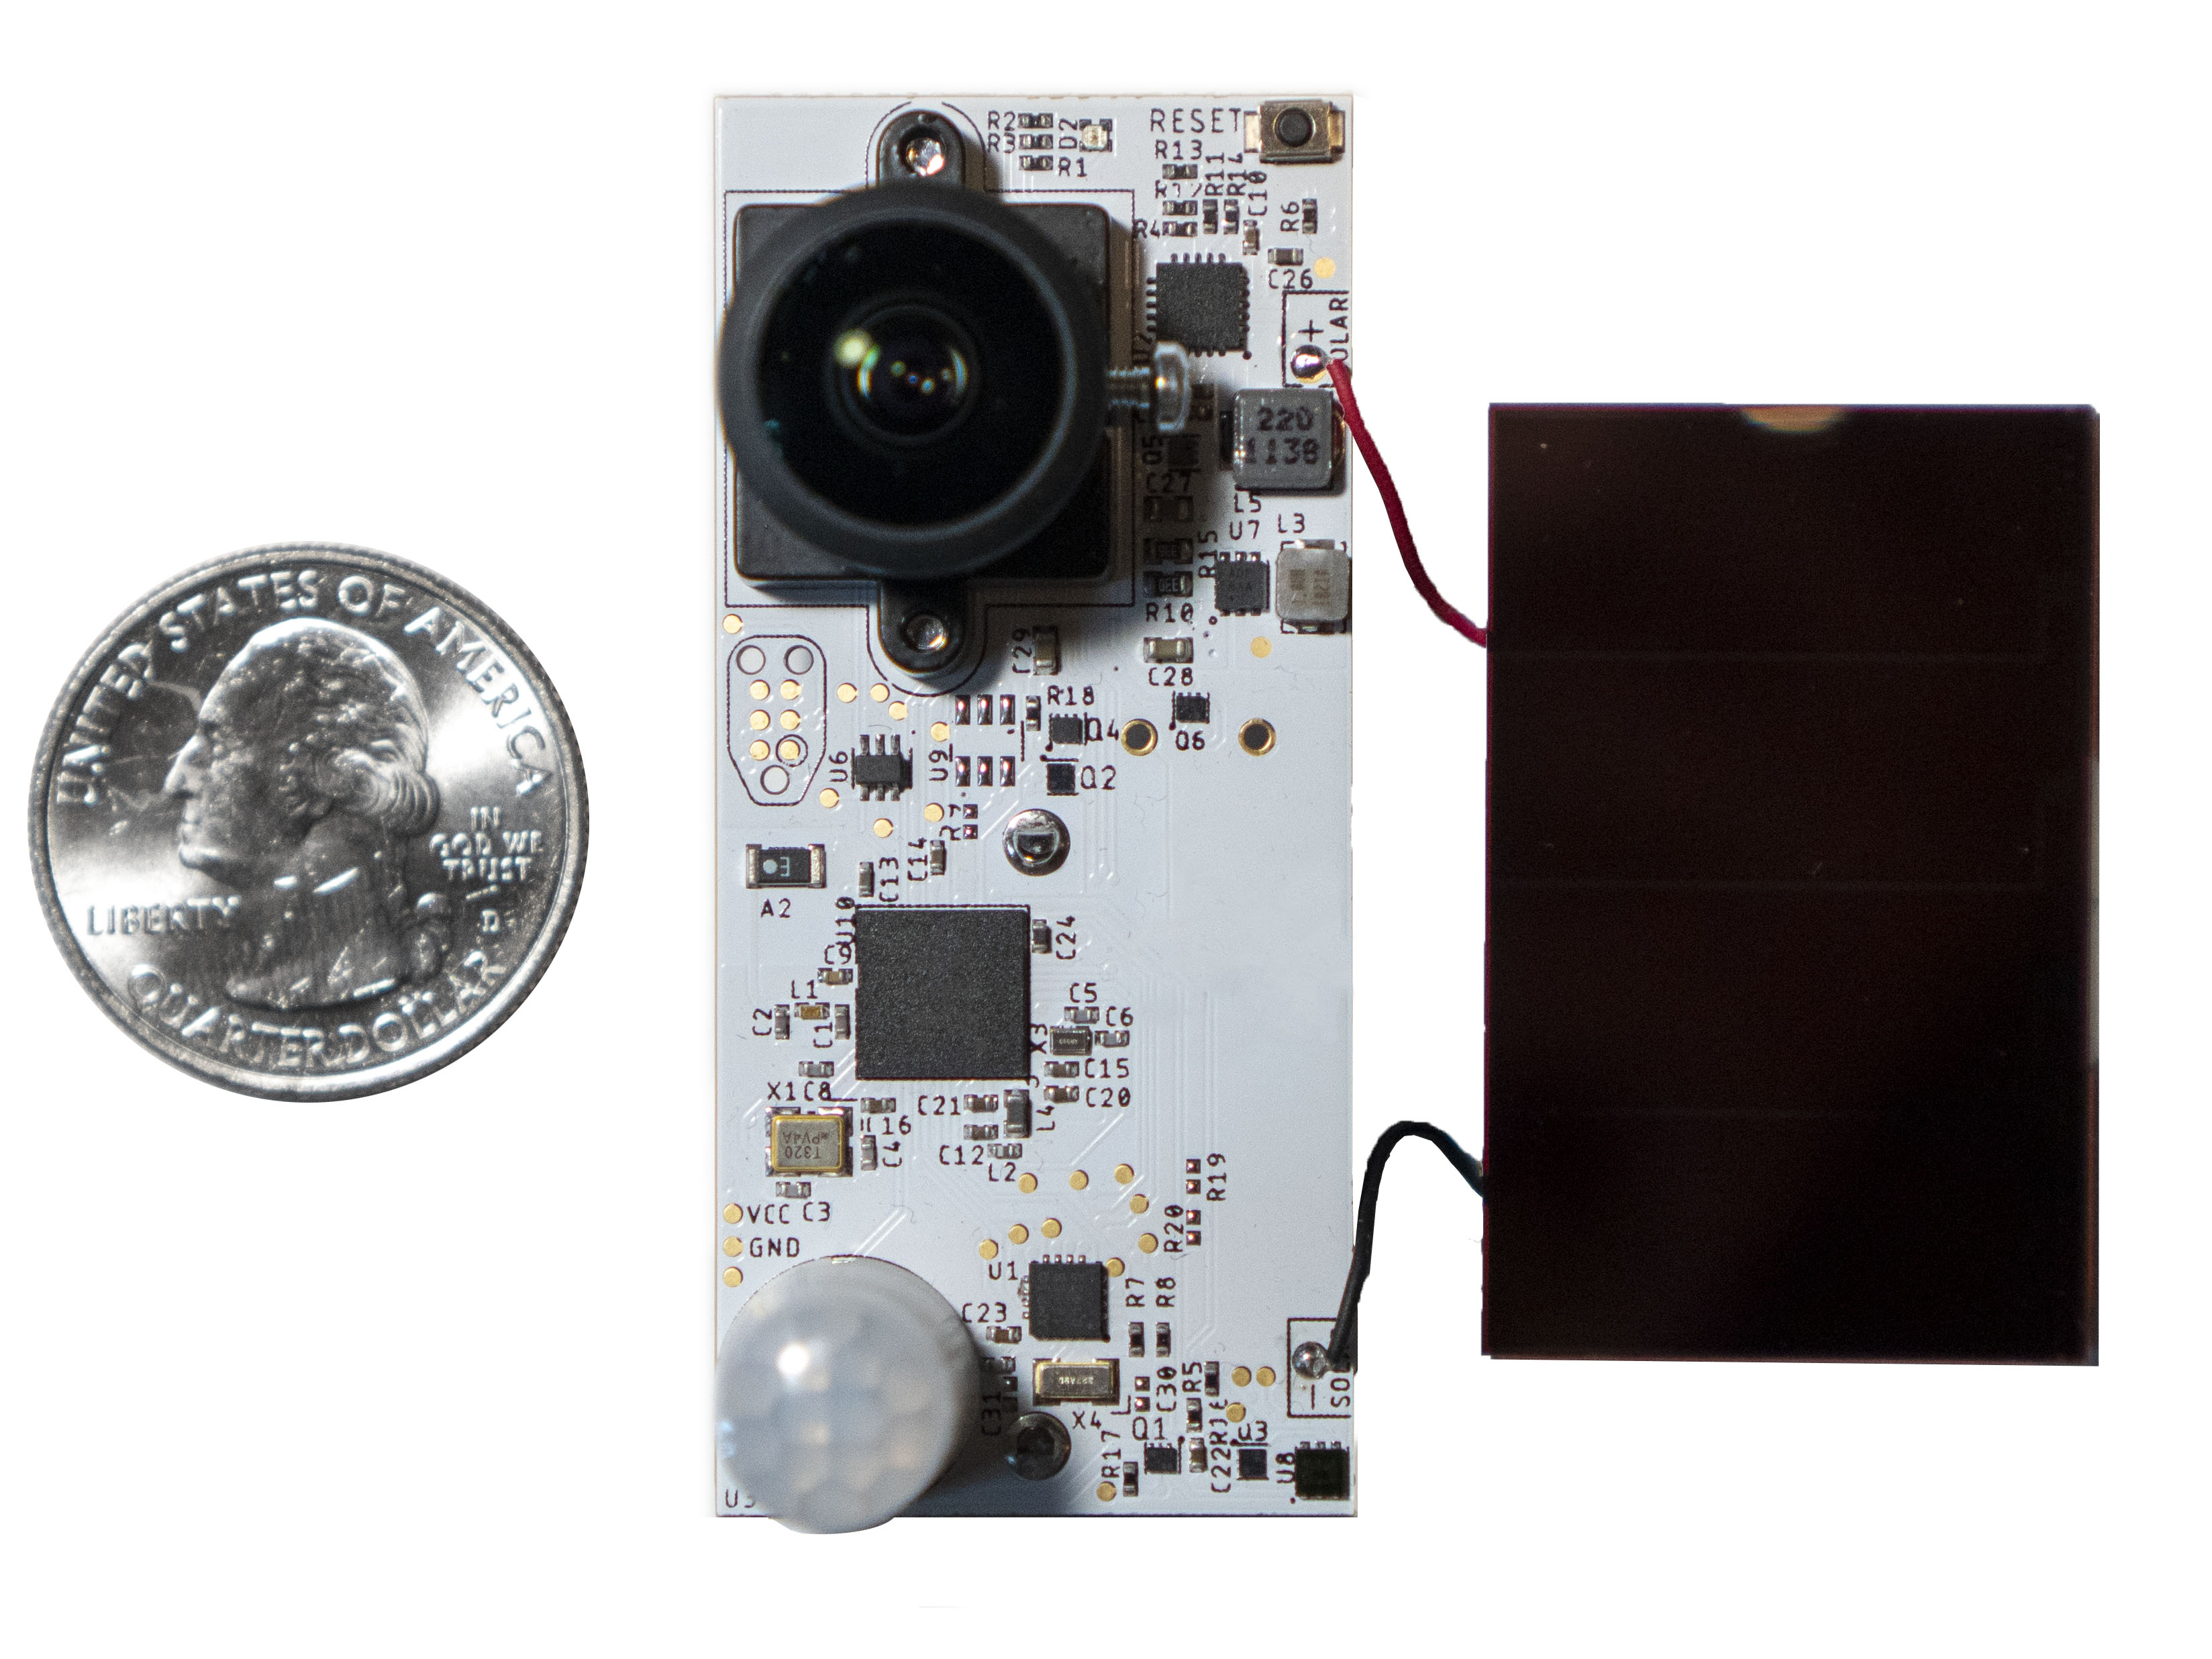
\includegraphics[width=\columnwidth]{images/platform_quarter.jpg}
\vspace{-2\baselineskip}
\caption{ \name{}. 
    \normalfont{A wireless camera platform for indoor computer vision applications. To achieve a multi-year lifetime, we employ energy harvesting with a photo-voltaic panel. A quarter is included for scale. \name is capable of local inference as well as full image transmission to cloud image processing pipelines. The platform is 10\,mm thick, and has a rechargeable and non-rechargeable battery on its backside}
}
\end{definefigure}
\placefigure{fig:platform}

\section{Introduction}
Image inference, including classification and object detection, has been one of the most active areas of computer science and machine learning research. However, due to the cost and difficulty of deploying wired cameras, applications based on continuous image sensing is untenable. This is especially true for indoor applications, where camera density must be higher for sufficient coverage.

Indoor wireless camera sensors have been heavily researched and commercialized over the past fifteen years, but due to the technology available at the time, as well as incompatibilities between design decisions and longevity, these platforms are typically limited to lifetimes of at most weeks to months~\cite{rowe2007firefly,rahimi2005cyclops,blinkindoor,wyzeoutdoor,josephson2019wireless}. 
Deployment of these platforms beyond small or temporary installations remain a challenge due to the cost of frequent battery replacement.
With the confluence of new and improved COTS technology, like low power processors, radios, and image sensors, it is worth revisiting the design of wireless camera sensors. 

Recent improvements in microcontrollers go beyond lower power \cite{kim2018system}. Processors now include hardware floating point support, single cycle multiplies, and data-parallel instruction (SIMD) support. The promise of new dedicated accelerators provides the potential of significant improvements in inference performance on low power systems~\cite{armm55,himaxwiseeye}. This has led to renewed interest in performing complex local inference on a battery budget, especially as transmitting large data like images is traditionally very expensive. However, radios have also become far more power efficient, which again muddies the conventional wisdom. Indeed, it is now much cheaper to transmit large data to a more capable system. Desktop or server class machines handily outclass their low power microcontroller and accelerator brethren on performance, providing the ability to perform more complex and accurate inference, if only data can be efficiently delivered to them.
%Regardless of recent improvements, microcontroller and accelerator performance will continue to pale in comparison to desktop and server class computing systems. 
This is especially true as memory has not scaled at the same pace as processing.
This rapidly changing design space points to a requirement for a flexible architecture and framework for thinking about what applications are most suited for local processing versus cloud offload.
% or data transmission.

In this work, we present \name, the first wireless, energy-harvesting camera platform capable of capturing and transmitting an image every ten minutes for half a decade in indoor environments.
\name represents a culmination of recent work on low power camera sensors~\cite{josephson2019wireless,nardello2019camaroptera,naderiparizi2015wispcam} and energy harvesting sensor platforms~\cite{jackson2019capacity}. \name features a hierarchical energy harvesting system that couples a small rechargeable battery with a backup non-rechargeable battery. This combination provides the system with a long and reliable lifetime. The longevity and reliability of the platform make it suitable for long-term, low-maintenance deployments. Images captured by \name are capable of driving applications based on object detection, like people counting or interaction tracking. With default, pretrained weights, an object detection model is able to detect a person in \name images from 20 meters away.

\name is capable of performing both local inference and transmitting full images end-to-end to more powerful systems. Local inference potentially requires less energy than image transmission, and also provides significantly better privacy guarantees. In cases where privacy is not as much of a concern, image transmission to a more capable endpoint increases the flexibility and performance of inference run on images. Privacy can still be guaranteed if images are transmitted only within a local network.
We examine the implications of both architectural choices with respect to capability, energy, and latency.

Our results show that on modern SoCs, transmitting images surprisingly enables longer lifetimes and improved inference. While this conclusion is unique to indoor wireless camera sensors 
whose footprints are not dominated by their energy harvester or storage, its general methodology can be applied to other application spaces as well.
%
Through this conclusion, we develop an end-to-end architecture that makes images captured by \name accessible to data collectors and application builders. \name provides a scalable and easily deployable method to quickly gather visual data for machine learning training or datasets. Images collected by \name are easily integrated into popular computer vision and machine learning frameworks like OpenCV, TensorFlow, and PyTorch. Using these tools, high level applications can be built to drive visual applications like building occupancy counting for more efficient energy management and critical infrastructure monitoring atop a long-lived deployment of wireless \name devices.

%Additionally, privacy is a serious concern, and we demonstrate that \name is capable of some local inference. In cases where applications require capability over privacy, images can be transmitted end-to-end to the cloud, or to a more local endpoint. 
%This provides the option to still maintain some privacy when transmitting images.




\include{background}
\chapter{Design Intuition for Energy Harvesting Systems}
\label{chap:intuition}

\section{Is Energy Harvesting Worth It?}

\placefigure{fig:intuition:eh_worth_it}

\section{Defining the Application Space}
The designed purpose of a wireless sensor is generally a simple one: measure some phenomena, optionally perform some filtering or calculation on that measurement, and transmit the results. 
This has been the prevailing archetype of research and industrial sensing since the inception of wireless sensor networks. 
The acceptable reliability, and reporting frequency is highly dependent on application requirements. Many safety critical or industrial applications require high reliability and frequent and immediate sensing and reporting. Conversely, an amount of unreliability, incomplete data, or reporting delay is acceptable in some citizen science sensing applications, where any data is better than no data.

This section seeks to better explore the design space of wireless sensors, especially with respect to how requirements on the kind of data being reported, the reporting frequency, and reliability, affect the requirements on the sensor power supply design. 

\subsection{Data type}

\subsubsection{Counting}

\subsubsection{Measurement}

\subsection{Reporting Frequency}

\subsubsection{Periodic}

\subsubsection{Reactive}

\section{A Taxonomy of Wireless Sensor Power Supply Architectures}
\label{sec:intuition_related}

Prior work regarding energy harvesting sensor systems can be broadly
divided into two categories: those which make use of intermittent computing
techniques and those which do not.
Intermittent systems often exist in a regime of unreliable and ultra low harvester power, where
operation and uptime are not guaranteed. As such, they often lose power and
reboot while intermittently working through a sensing task.
A wealth of work has been devoted to
making these systems usable and reliable.
Other energy harvesting systems, especially those deployed outside, have access
to significantly more harvestable energy and are able to store more of this energy
for later use, so they
do not use intermittent computing techniques to complete their workloads.
\subsection{Intermittent Sensors}
\label{sec:related:intermittent}

Energy harvesting systems that rely
exclusively on repeatedly buffering small amounts of energy to
operate are commonly referred to as intermittent systems.
Many choose to employ
capacitors as an energy buffer due to their theoretically infinite lifetime,
but are limited to small energy capacities, and are only as reliable and
lively as their source of harvested energy.
In situations of energy drought, 
these platforms often deplete their 
small energy stores, and lacking energy,
they power off and lose
state, potentially in the middle of an important operation or for an extended
period of time.
\\

\vspace{-6pt}
\noindent
\textbf{One-shot Intermittency.}
The Gecko and Monjolo platforms ignore the difficulties associated with
completing longer workloads and instead allocate
just enough capacitance to turn on and perform a simple task. Sometimes, the
rate of harvesting is the sensor itself~\cite{campbellEnergy14,
yervaGrafting12, debruin2013monjolo}.  However, this approach can require
tedious and non-standard optimization of the cold start process and is severely
limited in its simplicity. Performing any sensing or computing outside of the
hardware's intended use case is often not possible,
and it is difficult to distinguish sensor failure from a lack of energy.
\\

\vspace{-6pt}
\noindent
\textbf{Checkpointing.}
Other work in this space attempts to cope with
intermittency
by developing tools and
programming language primitives that allow %can perform
complex and energy intensive tasks to execute despite limited energy storage.
Intermittent-aware programming
models and compilers were developed to enable checkpointing and progress latching over
workloads that may require more energy than can be stored or harvested in a
reasonable time~\cite{lucia2015simpler, ransford2012mementos, hesterTimely17}. New debugging tools
spanning both the hardware and software domains
measure the energy required for specific code operations
and restore energy state during code breakpoints~\cite{colin2016energy}.
\\

\vspace{-6pt}
\noindent
\textbf{Hardware Hysteresis Management.}
In addition to intermittent software techniques,
hardware platforms have been developed to
increase availability and responsiveness through the fine-grained management
of capacitor charging hysteresis.
For these systems,
it is often assumed that the upper hysteresis threshold, the point at which a
charging device turns on, is the voltage at which a capacitor is full, and the
lower threshold, the point at which the system turns off or sleeps, is the minimum
operating voltage of components in a system.
Smaller capacitors can charge to an upper
threshold and turn on faster, but store less energy.  Hysteresis management
techniques attempt to combine different sized capacitors to
minimize charging time while also maximizing available energy.

The Flicker
platform employs federated
energy storage in which each peripheral has its own storage tuned to the task
it is expected to perform~\cite{hesterTragedy15,hesterFlicker17}. This has the
effect of allowing various components to charge their storage faster, as well
as isolating power failure to independent components.  The Capybara platform is
similar, but provides even more flexibility by dynamically resizing its banked
capacitor store to match the energy required by a task
~\cite{colinReconfigurable18}. This leads to the lowest possible cold start and
capacitor recharge times to support a given
operation.

We believe the assumption that operation should be coupled to full-swing hysteresis
is not valid
for many systems. Capybara does explore the possibility of setting an upper
threshold to less than the maximum voltage and using an adjustable bottom
threshold instead of dynamically resizing their capacitor store.
However, they disregard these options due to high voltage comparator
power and long cold start times, respectively.
While these decisions make sense in this context, the importance they place on cold start optimization
is specific to their design. Capybara's power supply has a significant
"power overhead of the power system" that limits the effectiveness of
sleeping. Due to this, they opt to fully discharge their storage on every
operation and optimize cold start.  In practice, if a system has the ability to
enter a low power sleep mode or power off, it can
avoid cold start and control its energy usage by willfully entering these
states. With this operating principle, the benefits of hardware hysteresis management
are limited to reducing cold start time and are workload independent.

These complex software and hardware solutions, while increasing usability and reliability, do not address the singular problem for capacitor-based energy
harvesting systems: in the face of plentiful harvestable energy, they are not
able to store the energy for later use (in times of energy drought).
As a result, they must
micro-optimize the little energy they have.  In many applications, if these
systems had sufficient capacity, they could instead adjust sensing rate and
workloads over periods of days or weeks.  We show that the energy captured
by these systems and their subsequent availability
could be substantially improved by using larger energy buffers.
\subsection{Non-intermittent Sensors}
\label{sec:related:nonintermittent}
Non-intermittent energy harvesting sensors
have largely existed in environments with plentiful harvestable energy
and have been designed with sufficient capacity to capture this energy. Some
devices have also embraced backup primary-cells to further ensure
reliable operation.  \\

\vspace{-6pt}
\noindent
\textbf{Rechargeable Batteries.}
Most examples of such devices are deployed outdoors.
For these systems, the obvious choice is to use secondary-cells, as they can
better capture a significant portion of copious solar energy
~\cite{jiang2005perpetual, kansal2007power, corke2007long, lin2005heliomote, adkins2018signpost}.
Most notable of this group is Prometheus,
which utilizes a supercapacitor as a short term energy store, and when full,
charges a backup rechargeable lithium battery~\cite{jiang2005perpetual}. At
the time of its design, lithium cells offered highly limited recharge cycles,
and by utilizing a supercapacitor, much of this
charge-discharge volatility was masked from the secondary-cell, extending its lifetime.
Rechargeable batteries have also been applied to indoor sensing.
The EnHANTs sensor uses an intentionally oversized NiMH
battery, with plans to eventually use a thin-film battery~\cite{margolies2015energy}.
While the choice to use batteries allows for more energy capacity,
NiMH and thin film chemistries offer poor
energy density and lower cycle life compared to lithium
based chemistries. DoubleDip and other sensors~\cite{martin2012doubledip,raisigel2010autonomous} use a
lithium-manganese battery.  DoubleDip notes that supercapacitors offer
lower energy density and higher leakage when compared to batteries, but admits
that the lithium-manganese chemistry suffers from low maximum output currents
and a limited number of charge-discharge cycles.
While the limitations of past batteries have slowed their adoption in
low energy harvesting scenarios, we claim that recent developments in battery
technology will enable higher capacity energy storage without these trade offs.
\\

\vspace{-6pt}
\noindent
\textbf{Backup Energy Store.}
Regardless of which energy store is used, energy harvesting systems will
experience some degree of intermittency. We advocate that a non-rechargeable
backup energy store can be utilized to mask this intermittency, cold
start electrical components, and provide consistent, reliable, and lively operation.
The only system we find that employs a non-rechargeable
backup is the Pressac line of capacitor-based energy harvesting sensors which
use battery backup to obtain an estimated 10 years of continuous operation
\cite{pressac}.  This work suggests that these sensors could significantly
increase their lifetime by using a larger secondary energy store.
There has been little
exploration on the benefits of this hybrid design and the use of
primary-cells to avoid intermittency, cold start harvesting circuits,
and provide baseline reliability.


\section{A Framework for Energy Harvesting Power Supply Design}
\label{sec:framework}
We seek to illustrate the design space for energy harvesting sensors in two
ways. The first defines an energy harvesting sensor framework to examine
when designs are feasible and when they require intermittent techniques to make meaningful forward progress.
The second examines dynamic income energy and device behavior through numerical
modeling and simulation.  The framework is based on three key metrics:
harvested energy income, workload, and capacity.
\placefigure{fig:framework}

\subsection{Sensor Regimes}
\label{sec:framework:regime}
The framework splits the design space into four main regimes: always on,
infeasible, checkpointing required, and no intermittent techniques required.
These regimes and their constraints are illustrated in \cref{fig:framework},
and explained in more detail below. \\

\vspace{-6pt}
\noindent
\textbf{Always On.} If the energy harvester supplies a sensor with
more power than the max power it will ever draw, then the device needs
no energy buffer capacity to remain operational. If this is not the case,
then a sensor must have some ability to buffer energy to use when its
operating power exceeds than the harvester input power.
\\

\vspace{-6pt}
\noindent
\textbf{Infeasible.} If the energy harvester supplies less power than
the system leakage, the energy buffer will never
charge. If the energy buffer capacity is less than the
energy required to perform a workload's largest atomic operation, with energy harvested
during the operation itself, then that operation will not have enough energy to
complete.  Neither of these designs will make forward progress and are
therefore infeasible.
Common atomic operations on energy harvesting sensors include sampling a sensor,
sending a radio packet, booting the processor, and performing a checkpoint.
\\

\vspace{-6pt}
\noindent
\textbf{Checkpointing Required.} If the energy buffer can
hold enough energy to perform atomic operations, but
not enough to complete
workloads composed of multiple, chained
atomic operations (such as sampling a sensor and then sending a radio packet), then
a mechanism for saving state and continuing progress on the next reboot
must be employed.
\\

\vspace{-6pt}
\noindent
\textbf{No Intermittent Techniques.} A sensor that has enough harvester
potential and energy capacity to complete a workload's longest non-atomic
operation can operate without checkpointing. Such systems also benefit as
energy devoted to checkpointing can be used for a workload instead.
\\

\vspace{-6pt}
\noindent
\textbf{Hysteresis Management.}
Finally, if a sensor's deep sleep power draw %willfully powers down
is a substantial fraction of the harvester power, as
is the case with Capybara~\cite{colinReconfigurable18}, then it is
beneficial to continue operating until the energy
buffer is depleted, power off, and recharge quickly
rather than stop early and recharge slowly.
Under this scenario, hysteresis management techniques,
such as reconfigurable capacity and federated energy can increase sensor
performance as discussed in \cref{sec:related}.
The utility of hysteresis management is diminished
when the ratio of harvester power to deep sleep power increases.
For sensors that can willfully power off or sleep,
operating thresholds can be controlled, disentangling
capacity and charging hysteresis.
Their deep
sleep power is equal to leakage, and such techniques
will not improve recharge times.

For all systems, these techniques can decrease cold start time
by reducing the capacity that must be charged
to achieve cold start.

This is more beneficial for systems that cold start frequently and
have a higher energy capacity, however,
a higher-capacity energy store also has a lower probability of
needing to cold start. Therefore the benefits of hysteresis management for
cold start with respect to storage capacity are in conflict with their necessity,
and we do not attempt to quantify these subtle nuances in \cref{fig:framework}.

\subsection{Framework Limitations}
\label{sec:framework:limitations}
This framework makes a couple simplifying assumptions that prevent it from
fully capturing the richness of the design space.\\

\vspace{-6pt}
\noindent
\textbf{Backup Energy Store.}
This framework does not consider the impact of a backup energy store.
%that is pre-charged before the sensor begins operation.
%The simplest way
%to view
A backup energy store can be viewed as the ability to inject additional energy
to the system at arbitrary times,
%move the system
%outside of the regime of requiring checkpoints for very energy intensive operations, or
eliminating the need for checkpointing when there is very low
harvesting potential.

A backup energy store could also contribute in more subtle ways. It could
allow a system to avoid the energy and complexity of checkpointing by
providing just enough energy for a deep sleep mode with state retention rather
than a full power down when the system depletes its stored energy. It could also
cold start energy buffer charging to eliminate the need for reconfigurable
power supplies, or to increase the efficiency of
the energy harvesting front-end at low voltages.
Finally, in periods of long energy drought, the backup energy store could increase
sensor availability.

While the use of a backup energy store
does constrain the sensor to a finite lifetime,
%especially since current technology favors non-rechargeable, primary-cells as
%backup energy stores,
energy harvesting can substantially extend these lifetimes under certain harvesting
conditions.\\
%We explore the lifetime of energy harvesting
%designs with backup energy stores in \cref{sec:primary}.

\vspace{-6pt}
\noindent
\textbf{Constant Harvester Power.}
The framework assumes an energy harvester will supply a constant energy
income, when in reality income is often highly variable. In practice, a sensor
platform both defines the regions of the plot, and occupies a
vertical line which represents the energy storage capacity of the sensor
combined with the range of harvester input powers it might experience. We expect
this line will span multiple regions for most sensors.

However, by ignoring variability, the plot also fails to illustrate key benefits
of capacity under varying energy incomes and workloads. Intuitively,
higher energy buffer capacity can store energy in times of excess and supply
that energy in times of drought. This balancing out of energy income
effectively raises the minimum power supplied by the energy harvester.
Because the extent of this impact is completely dependent on the variability
of the energy income and workload of the sensor, we also develop a numerical simulation to
quantify the impact of capacity
on key metrics including energy utilization, availability and reactivity.

\section{Application feasibility}

\section{An Intuitive Case for Capacity}

\begin{definetable}{tab:related}
  \scriptsize
  \begin{threeparttable}
  \centering
  \begin{tabular}{l | c c| c c| c}
      \multirow{2}{*}{Platform} & \multicolumn{2}{c|}{Successful Events\,(\%)}  & \multicolumn{2}{c|}{\parbox{2.5cm}{\centering Long-Running\\Time to Completion Ratio}} & \multirow{2}{*}{Lifetime\,(yrs)}\\
                              & Periodic     & Reactive                     & Average & 95th Percentile & \\
    \hline
    Telos \cite{polastre2005telos}                      & 100   & 100   & 1     & 1     & 8.55\\
    Hamilton \cite{kim2018system}                & 100   & 100   & 1     & 1     & 6.75\\
    BLEES \cite{adkins2015michigan}                     & 100   & 100   & 1     & 1     & 1.11\\
    Gecko \cite{yervaGrafting12}                 & 39.5  & 64.9  & 387   & 981   & $\infty$\,\tnote{g} \\
    Capybara~\cite{colinReconfigurable18}\,\tnote{a}    & 46.3  & 72.8  & 37.6  & 1     & $\infty$\,\tnote{g}\\
    Capybara~\cite{colinReconfigurable18}\,\tnote{b}    & 41.1  & 67.1  & 2730  & 8900 & $\infty$\,\tnote{g}\\
    Flicker \cite{hesterFlicker17}                      & 39.3  & 64.2  & 1307  & 5670 & $\infty$\,\tnote{g}\\
    EnHANTs \cite{margolies2015energy}                  & 79.4  & 96.0  & 1     & 1     & \textemdash\,\tnote{h}\\
    DoubleDip \cite{martin2012doubledip}                & 77.9  & 66.5  & 1     & 1     & \textemdash\,\tnote{h}\\
    \cite{raisigel2010autonomous}                       & 78.4  & 66.9  & 1     & 1     & \textemdash\,\tnote{h}\\
    \textbf{\name}\,\tnote{c}                           & 81.2  & 98.3  & 1     & 1     & \textemdash\,\tnote{i}\\
    \textbf{\name}\,\tnote{d}                           & 100   & 100   & 1     & 1     &  35.8\\
    \textbf{\name}\,\tnote{e}                           & 100   & 100   & 1     & 1     &  30.2\\
    \textbf{\name}\,\tnote{f}                           & 100   & 100   & 1     & 1     &  6.27\\
  \end{tabular}
    \begin{tablenotes}[para]
      \item[a] With capacitors: 400\,\si{\micro\farad} ceramic + 330\,\si{\micro\farad} tantalum + 67.5\,mF supercapacitor.
      \item[b] With capacitors: 300\,\si{\micro\farad} ceramic + 1100\,\si{\micro\farad} tantalum + 7.5\,mF supercapacitor.
      \item[c] No primary-cell.
      \item[d] AA primary-cells like Telos.
      \item[e] CR123A primary-cell like Hamilton.
      \item[f] CR2032 like BLEES.
      \item[g] Lifetimes are theoretically infinite for capacitor-based systems.
      \item[h] Not enough information to predict cycling failure time for theses systems.
      \item[i] Expect cycling failure in 20-50 years, but do not attempt to estimate.
    \end{tablenotes}
  \end{threeparttable}
  \caption{
  \normalfont
      Modeled performance of energy harvesting systems.
    For each  platform considered, we model the performance of its energy storage
    architecture. Periodic workload and lifetime estimates are based on a 10\,s
    period, and the reactive workload is scaled to
    generate a maximum of 2000 events per hour (3.4\,s average daily period). Generally,
    intermittent systems have significantly worse availability and responsiveness compared to
    battery-only systems and systems that use a secondary-cell. Battery-only
    systems achieve perfect operation, but have finite, sub-decade lifetimes.
    }
\end{definetable}

\begin{definefigure}{fig:framework}
  \centering
  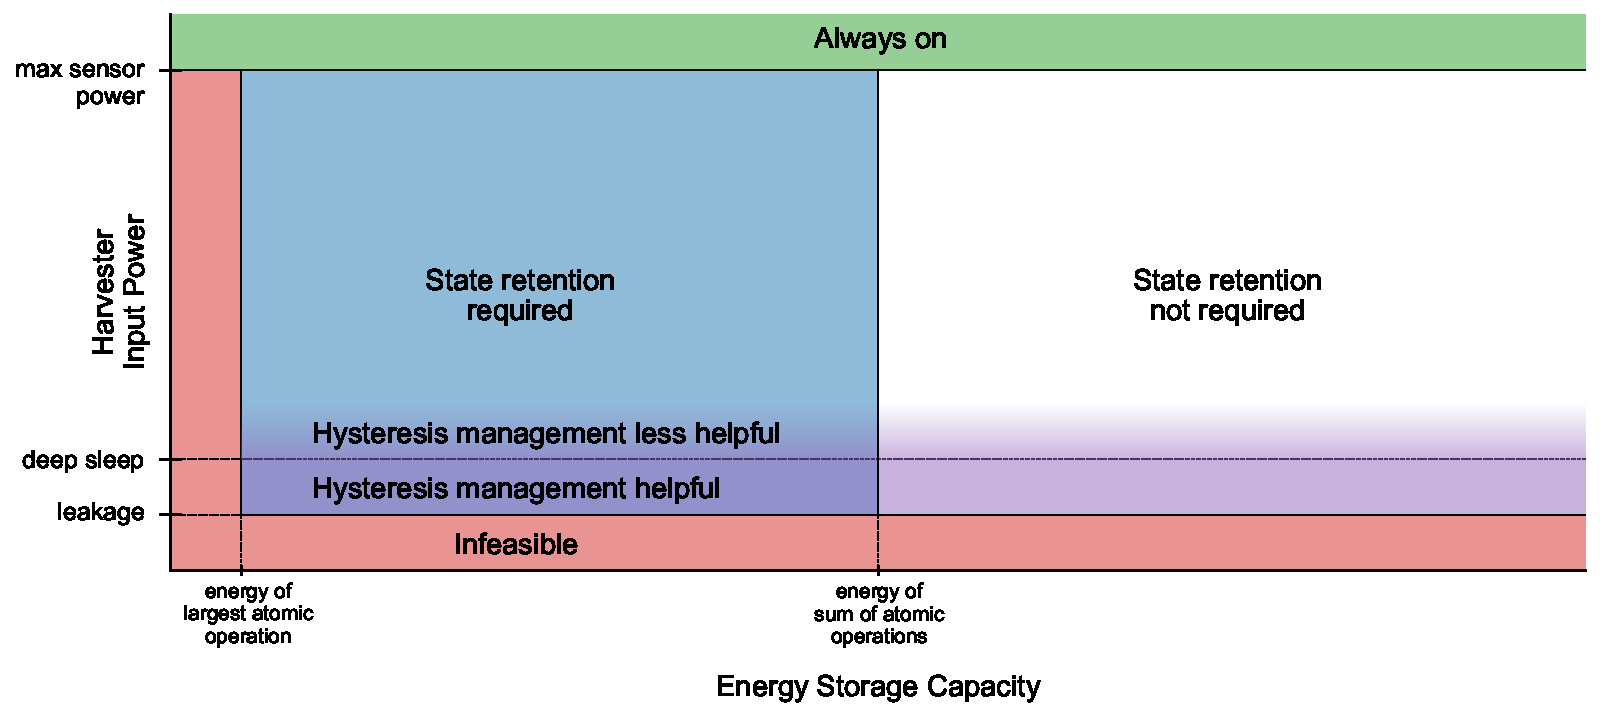
\includegraphics[width=\columnwidth]{figs/capacity/harvesting_framework/framework}
  \caption{
  %Energy harvesting
  %sensors have different capabilities and requirements
  \normalfont Design space for energy harvesting sensors based on their energy
  income (which we assume is constant for this analysis), energy storage capacity, and workload.
  Workload is represented by the largest atomic/non-atomic operations supported
  by a design, as well as the deep sleep and leakage power.  The plot breaks
  into four regions: \textbf{1)} always
  on or effectively powered, \textbf{2)} Infeasible due to lack of energy storage or
  leakage higher than harvesting rate \textbf{3)} Feasible but requires checkpointing
  to make forward progress, and \textbf{4)} Enough energy storage to not require
  or benefit from checkpointing. Additionally, sensors which have high
  power when they enter deep sleep before depleting their
  energy buffer may benefit from hysteresis management techniques.
  This benefit diminishes with lower sleep currents and higher harvesting potential.
  %With increased capacity, sensors can avoid the complexity of intermittent
  %programming techniques and specialized, reconfigurable power supplies in addition
  %to the other benefits of increased capacity discussed
  %in \cref{sec:store}.
  }
\end{definefigure}


\begin{definefigure}{fig:intuition:eh_worth_it}
  \centering
  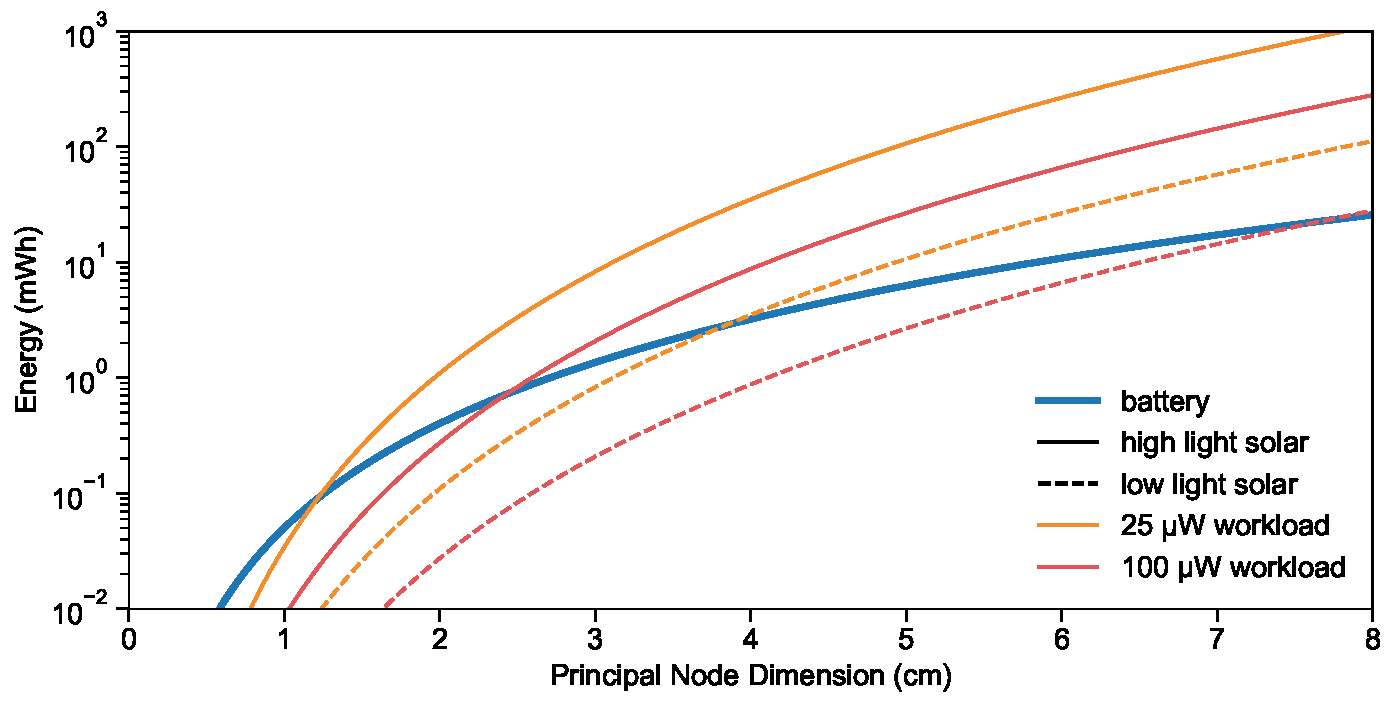
\includegraphics[width=\columnwidth]{figs/is_eh_worth_it.pdf}
  \caption{
  blah
  }
\end{definefigure}
\chapter{Exploring Energy Utilization and Reliability Through Simulation}
\label{cha:capacity}

\section{Modeling the Common Case}
\label{sec:overview}
The framework we have presented does not consider
harvesting and workload
variability.
To explore the dynamic effects that energy
capacity and backup storage have on sensor performance in the face
of variability, we develop a simple numerical model.
We use representative environmental conditions, measurements of real hardware,
and synthesized workloads to determine the common case for our model and simulate
the behavior of energy harvesting sensors. From these data, our model
produces estimates of energy utilization, availability, responsiveness, and
lifetime.
\\

\vspace{-6pt}
\noindent
\textbf{Environmental Conditions.}
We assume an indoor environment
that is built for and used
by people.
Occupied indoor environments are the focus of a significant
amount of
prior work, 
and for good reason: most
applications aim to improve the lives of people and are necessarily present
in the spaces they occupy. Even the example applications of intermittent,
energy harvesting systems are nearly all centered around monitoring
indoor and human-centric phenomena~\cite{hesterTimely17,hesterFlicker17,colinReconfigurable18,campbellEnergy14}.
We expect our environment to be lit, and that it may
occasionally get direct or indirect sunlight. We use
indoor photovoltaic energy harvesting because under these conditions,
it offers an order of magnitude more energy than other methods.
This does not mean that the conclusions we draw are not applicable to other
environments and harvesting methods, but that the sizing and lifetime
conclusions may be different.

To model the harvestable light in an occupied indoor environment, we use
the EnHANTS indoor irradiance dataset~\cite{gorlatova2013networking}. We
find that it is the most complete and extensive dataset for indoor light
irradiance traces, capturing over a year of data in several situations.
The traces we use for our model are summarized in \cref{tab:capacity:rep}.\\

\vspace{-6pt}
\noindent
\textbf{Representative Hardware.}
We limit our analysis to the effects of capacity,
independent of the differences of energy intensity or efficiency in device
component selection. To do so, we define an example solar energy harvesting
sensor platform that utilizes available, state-of-the-art, commercial
components.
\placefigure[t]{tab:capacity:rep}
We choose new
components in an attempt to better represent prior energy storage designs and
give them the benefit of the improvements that have occurred in recent years.
We take benchmark
measurements of various tasks performed by this platform, such as the
amount of time and energy required to sample a sensor or send a Bluetooth Low
Energy (BLE) packet. These benchmarks are used to generate energy utilization metrics
for our representative workloads shown in \cref{tab:capacity:rep}.
The physical size of the solar panel used by this sensor
is assumed to be
10.9~cm\textsuperscript{2} and the volume of the sensor node is similar to prior
work like the Hamilton sensor~\cite{kim2018system}.
We implement this design and describe it further in \cref{sec:impl:permamote}.
\\

\vspace{-6pt}
\noindent
\textbf{Representative Workloads.}
We find that sensing workloads generally fall into three
categories: (i) periodic sense-and-send~\cite{mainwaring2002wireless}, (ii) reactive event detection~\cite{campbellEnergy14}, and (iii) infrequent,
long-running, high-power events~\cite{levis2004trickle}. We choose a representative workload for each
of these categories to use in our model.
We characterize our ``periodic sense-and-send''
workload as periodically sampling a light and color sensor and sending a
BLE
advertisement containing the data.
Our ``reactive workload'' is
represented by sending a BLE advertisement upon motion detection of the main
entrance of a university building, and we linearly scale the frequency
of these events to represent varying amounts of usage. We treat these
workloads as atomic.  Finally, our ``infrequent expensive'' workload is a
contiguous
task that is representative of an
over-the-air firmware update, which is randomly executed with an average occurrence rate
of once every two weeks.
We conservatively assume these long running tasks can be interrupted
and resumed at any point during execution and that any checkpointing is free.
\\

\vspace{-6pt}
\noindent
\textbf{A Predictive Model.}
We use the previously discussed indoor irradiance traces, generalized
workloads, and hardware characterizations to model the behavior of sensors
using different types and sizes of energy storage. We develop an open
source\footnote{\url{https://github.com/lab11/permamote/tree/master/simulator}}
numerical model that allows parameterization of various system
characteristics, including regulator efficiency, solar harvester size
and efficiency, energy storage capacity, leakage, ESR, and charge-discharge
efficiency. These parameters are summarized in \cref{tab:parameters}.

The simulation of our model operates as a second-by-second calculation of the
amount of energy entering and exiting a device.
At every step, the simulation calculates the net energy gain or loss of the
system based on its current state and available stored energy.  Occasionally,
the model performs a workload event based on either a periodic schedule (in the
case of a sense-and-send workload) or from a random distribution (reactive
event detection or a high-power event). For our modeling, workload schedules
are generated from values listed in \cref{tab:capacity:rep}.
This simulation is performed for the entirety of an
input irradiance trace, which constitutes about a year of data. During
a simulation, metrics such as energy utilization, the fraction of completed
events versus expected events, and events' time to completion are collected,
and if applicable, the primary-cell lifetime is estimated from a trace of its

During simulation, modeled devices can be online or offline and idle or performing
work. These states are shown in \cref{fig:statemachine}.  A device's state
transitions from top to bottom of this figure and vice versa depending on the
energy state of the secondary storage.
If the secondary-cell energy state drops below \texttt{min\_hyst},
the state of the system moves to the upper
half (offline) of this diagram. The state of the system moves downward (online)
if the state of charge of the secondary reaches the \texttt{max\_hyst}
limit. Secondary charging hysteresis limits are defined by parameters described in \cref{tab:parameters}.
A device's state can also move
to the right or left of the state machine depending on whether a workload event
is scheduled, or the prescribed workload has been completed. A new
workload event is counted as failed if the device is not in the \textsf{Online
Idle} state when it begins.
In the case of the ``atomic''
sense-and-send and reactive workloads, the modeled device will only begin
to perform an expected workload event if it has
enough energy to perform the event in entirety. If the workload is not atomic,
the device will only begin scheduled work if it has enough energy to make the
configured minimum amount of progress. We
make the assumption that the duration of atomic events are less than the one
second simulation step.
We assume that a modeled sensor has perfect, zero-energy progress
latching and can go to sleep at any point after an active event. If
there is energy remaining after performing a task, the modeled sensor will
attempt to spend the rest of the simulation period in the \textsf{Online Idle} state.

If the simulated device is configured with a backup primary-cell, offline
states transform to "primary" states in which the device remains on and
able to perform work, but charges energy usage to the primary storage instead
of the secondary. During these periods, the secondary cell continues charging
from harvested energy. Upon reaching the upper charging hysteresis
limit, the device returns to an online state, using energy stored in the
secondary.  If the primary storage is depleted, the simulation ends early.

\placefigure[t]{tab:parameters}
\placefigure[t]{fig:statemachine}
\placefigure[t]{fig:usage}

\section{Capacity Increases Energy Capture}
\label{sec:store}

In addition to relaxing the need for intermittent techniques, we find that
an increase in sensor energy capacity
achieves a significant return on sensor
reliability and capability in the face of variable energy income.  Higher
energy capacity allows higher energy capture during periods of abundant
harvestable energy.

\subsection{Ambient Energy Utilization}
\label{sec:store:utilization}

Ambient energy is underutilized when it is not used to support the specified
sensing application. This may happen for two reasons: 1) the secondary
energy store is full but energy is still available for harvesting, and 2) the
sensor performs work based on its energy state rather than its application
goals. The first scenario is common for energy harvesting systems
presented in prior work, which charge up a capacitor and wait for an event
before sensing and sending, failing to capture all energy that may
have been harvested while their capacitor was full~\cite{campbellEnergy14}.
For an example of the second scenario, consider
systems that transmit a packet every time their energy storage capacitor
is full rather than saving this energy for use during periods of lower harvesting
potential~\cite{hesterFlicker17, colinReconfigurable18}. Another example of this are sensors in which the harvesting
rate is proportional to the sensed phenomena~\cite{debruin2013monjolo}.
While compelling for their simplicity, these sensors use
energy that could be saved and used
later for more useful and relevant tasks.

To explore ambient energy utilization as a function of storage size, we
model the charge-discharge patterns of idealized energy stores under
the harvesting conditions and workloads described in \cref{sec:overview}.
This modeling is primarily accounting for our first classification of
wasted energy, since our workload definitions \textit{do not} perform
tasks in response to available energy; instead they attempt to maximize the success
rates for the specified sensing tasks.
The results of this modeling are shown in \cref{fig:usage}. No matter
the amount of available energy, utilization increases as
storage capacity increases. For scenarios with low harvesting potential and high
power workloads, a sensor with at least 1\,mWh of storage can accomplish 100\% utilization.
In cases of
high harvesting potential and low power workloads, utilization often
stops increasing before reaching 100\%. This
can be attributed to a small fraction of the available energy being sufficient
to fully support the sensing task.
Small increases in utilization
have significant impact on reliability and system lifetime.
\placefigure[t]{fig:reliability}

\subsection{Application Reliability}
\label{sec:store:reliability}

We also model the ability of varying energy stores to meet our defined
sensing tasks and intensities. Our results are
shown in \cref{fig:reliability}. 
Similar to the results of \cref{sec:store:utilization}, we see marked
increases in performance when energy stores reach 1-10\,mWh
of capacity.
Simulations experience 100\% reliability for all but
the most energy constrained scenarios with high power workloads and
$\geq$2\,mWh of energy storage.
We also see that even when low capacity sensors
have large energy harvesting potentials and infrequent workloads, they experience low
reliability.
This is because they
do not have enough storage to keep sensing throughout the night.

Finally, we analyze the ability of different storage configurations to perform a
random, contiguous, higher energy task. We use a 100\,mJ (30\,\textmu Wh) event that is representative of a
50\,KB over-the-air code update. While this is larger than a code update would be
for simple programs,
we see in \cref{fig:reliability:otattc} that nearly all of the configurations with
0.28\,mWh of energy storage complete the task in the minimum time (5\,s). In comparison,
even reducing the amount of energy storage to match the amount of energy
required for the code updates causes significant latency. It is clear that
many of the updates for smaller energy storage configurations
do not complete for 1000-10,000\,s.
This aligns with the amount of time a sensor may sit
idle overnight waiting for solar power.

% Mayfly/Flicker
% - Timekeeper: 1 10uF 0805YD106KAT2A 0.09 @ 100 (equiv 0.03 @ 100) (0.023)
% - MCU: 1 22uF Not specified, but an AVX 1210 costs 0.44 @ 100 (equiv 0.079 @ 100) (0.025)
% - Acel 1 2.2uF EMK107BJ225KA-T 0.039 @ 100 (equiv 0.036 @ 100) (0.015)
% - BLE  1 47uF GRM31CR60J476ME 0.21 @ 100 (equiv 0.16 @ 100) (0.028)
% - HUM  1 15uF C2012X7S1A156M125AC 0.37 @ 100 (equiv 0.19 @ 100) (0.052)
% - Press 1 33uF C3216X5R0J336M130AC 0.44 @ 100 (equiv 0.38 @ 100) (0.034)
%
% Capybara
% - test 1: 400uF ceramic (4x100 0.31 equive @100) (0.043), 330uF tant (0.69 equiv @100) (0.24), 67.5 mF super (?? $21?, $2.42)
% - test 2: 300uF ceramic (3x100), 1100uF tant ($2.43) (0.62), 7.5 mF super ($2.42) (
% - test 3: 300uF cerami (3x100)c, 100uF tant ($0.28) (0.17), 7.5 mF super ($2.42)
%
% Gecko Power Supply
% - 5 TLJG227M004R3000 1.39 @ 100 (0.37 equiv, 0.16 ali)
%
% Wisp
% - 1 10uF ?? $0.05 @ 100
\begin{definefigure*}{fig:primary}
  \centering
  \begin{subfigure}{0.39\textwidth}
    \centering
    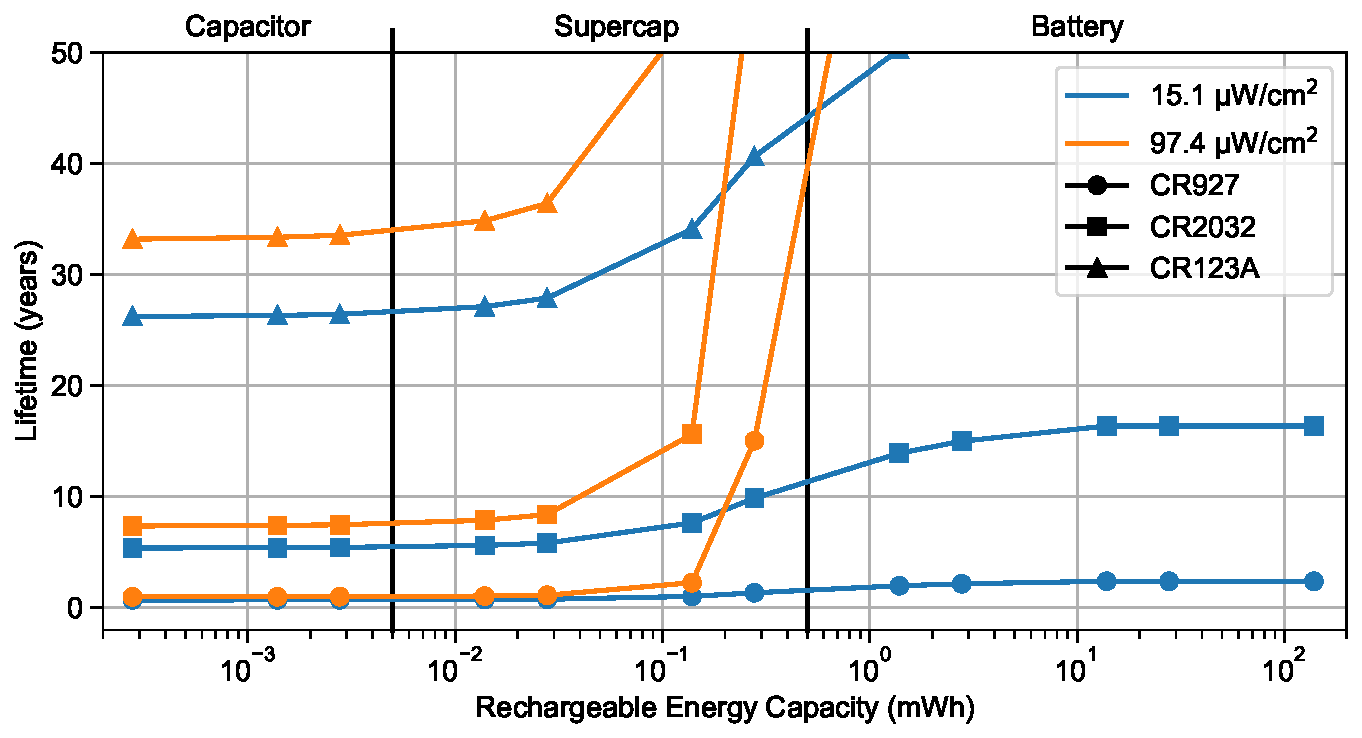
\includegraphics[width=0.85\linewidth]{figs/capacity/primary/sense_and_send_life_vs_sec_size}
    \caption{Periodic Application}
    \label{fig:primary:sensesec}
  \end{subfigure}
  \begin{subfigure}{0.6\textwidth}
    \centering
    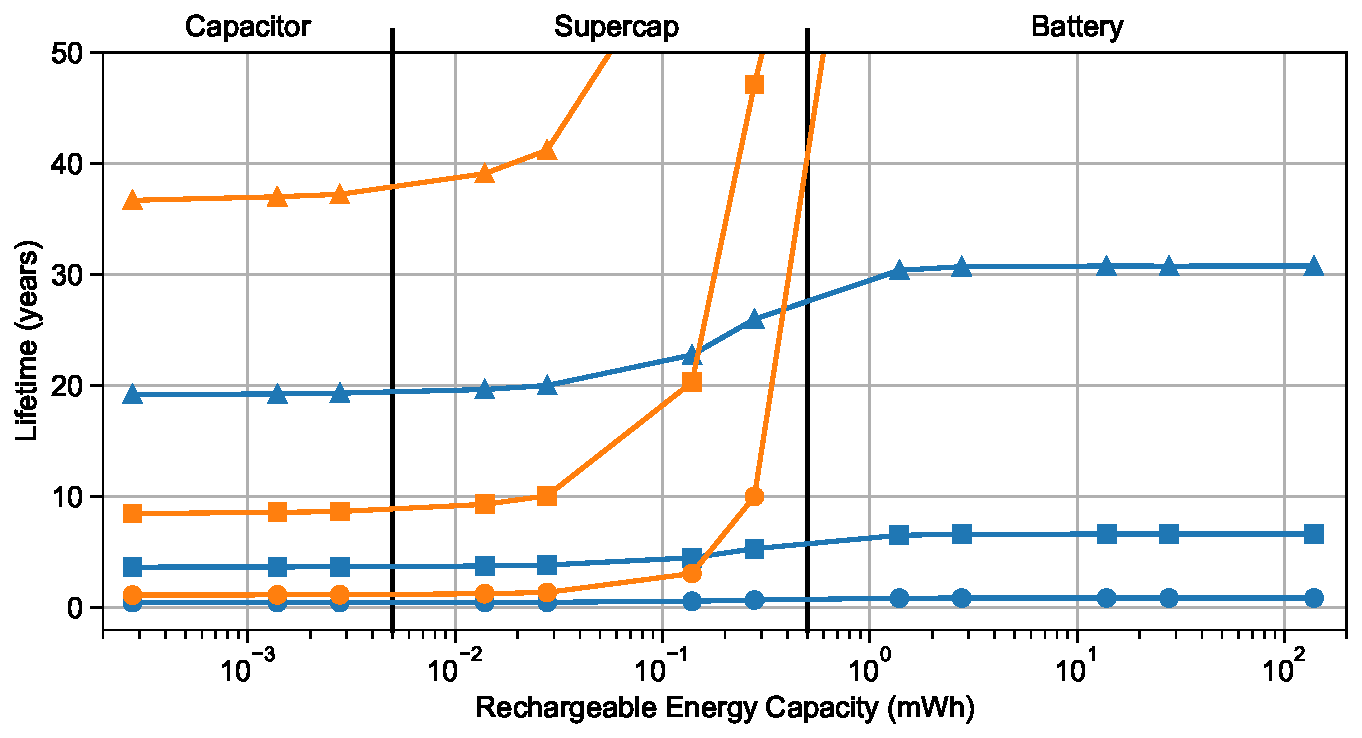
\includegraphics[width=0.85\linewidth]{figs/capacity/primary/door_occu_life_vs_sec_size}
      \caption{Reactive Application}
    \label{fig:primary:eventsec}
  \end{subfigure}
  \caption{
    \normalfont
    Estimated lifetime
    when varying secondary energy capacity for different harvesting scenarios
    and backup energy storage sizes. The periodic application's period
    is 30\,s and the reactive application events are scaled to
    represent a maximum of 2000 events per hour.
    %Harvesting scenarios and workloads
    %are described in \cref{sec:overview} and \cref{tab:capacity:rep}, and
    The backup
    sizes correspond to those found in common coin cell batteries:
    90\,mWh, 720\,mWh, 4500\,mWh for the CR927, CR2032, and CR123A respectively.
    As the ability to capture
    more harvested energy increases, the sensors lifetime increases.
    In some scenarios, expected
    lifetime becomes unbounded as the device is able to subsist entirely on harvested
    energy.
    %All scenarios experience substantial
    %increases in lifetime from increased secondary storage size.
    We see a 2-4x increase in lifetime estimates from the smallest to largest
    capacity simulated, if we only consider bounded results.
    We emphasize that
    these lifetime estimations are
    just estimations, and while we do model the 1\,\%/year leakage
    typical of coin cells, we do not consider the unknown
    physical degradation that would be experienced over decades of use.
    }
\end{definefigure*}

\section{Necessary Reliability}
this section will be about achieving .99, .999, and 100\% reliability, assuming sufficient \textit{average} energy. What is the cost in energy capacity?

\section{100\% Reliability Requires Backup}
\label{sec:primary}

Increasing secondary capacity greatly improves
reliability.
%for both periodic and reactive workloads.
However, some environmental
conditions and workloads do not reach 100\% reliability regardless of the size
of the secondary store.
%reactive workloads with large secondary
%capacities, some of the
Some results in \cref{fig:reliability}
appear to achieve perfect reliability, but still miss 0.1-2\% of events.
%with
%diminishing returns for increased secondary capacity.
%Additionally, some workloads
Others achieve well below 100\% reliability, %at the upper extents of storage capacity,
and simply require much more energy
than is harvestable. A backup energy store can increase reliability of a system
to 100\%, at the cost of a finite lifetime.
%In both of these case, further increasing secondary
%capacity does not improve reliability.
%and the desired application cannot rely soly on harvested power.
%and we expect that
%workloads which achieve slightly less than perfect reliability are experiencing
%a combination of brief harvesting droughts and high amounts of temporally local activity
%that push the local average power well above that of the average harvested power.
%While the second case may be solved with a sufficiently large secondary-cell, the
%diminishing returns of increasing secondary size and
%unpredictability of some reactive applications
%makes it difficult to rely solely on harvested power.

\subsection{Reliability Required}
\label{sec:primary:reliability}

We argue that 100\% reliability is a significant improvement over
even low failure rates with respect to reliability
%information
%for many applications
and simplicity due to the lack of intermittency.
%that is a consequence
%of reliability.
Many applications, especially human facing ones,
must be reliable to function, and research shows that unreliability
leads to frustration and %lack of
unwillingness to adopt automated solutions~\cite{brushHome11, edwardsHome01, shehanHome07}.
To use energy harvesting sensors for control or feedback of systems with potential
safety issues, inherent unreliability is intolerable.

Worse, intermittent system failures are difficult to detect %and mitigate
because there is no method for distinguishing between lack of energy
and an actual fault. While scheduled communication of current energy state
may help, this would be difficult for systems that only store enough
energy to perform a single operation such as Flicker~\cite{hesterFlicker17},
Gecko~\cite{yervaGrafting12}, and some configurations of
Capybara~\cite{colinReconfigurable18}.

Finally, it is more difficult
to program intermittent systems because programmers or the underlying
programming model must monitor and adapt to available energy with fine
granularity, both of which are non-trivial tasks.
These systems have little ability to correct for failures
even when they are detected.
%A reliable system has the ability to spend more short-term
%energy to correct for detected failures.

\subsection{Lifetime of a Backup Energy Store}
\label{sec:primary:lifetime}

To achieve 100\% reliability and avoid intermittency,
designs can utilize a backup energy store.
%that is pre-charged at the start of the
%node's life.
In instances where the rechargeable source is depleted, the system
can operate from the backup, masking the effects of variable energy income.
When the backup energy store is depleted, we consider the node's lifetime
to be complete, although it could continue
operating intermittently and with lower reliability. This energy store should
be a primary-cell, as they offer very low self-discharge, long shelf life, and
substantial energy density.
%This pre-charged energy store could be accomplished
%by either a large secondary-cell or a primary-cell, but to avoid increasing
%volume significantly this energy store will almost certainly manifest itself
%as a non-rechargeable battery.

An analysis of the reliable lifetime of a node with both energy
harvesting and a backup energy store is shown in \cref{fig:primary}.
%for
%both periodic and event based workloads.
We choose several backup energy
stores with energy equivalent to those found in several types of common
primary-cells. We see that with energy harvesting and a sufficiently
large secondary energy store, nodes can
achieve 100\% reliable lifetimes that exceed
what we can reasonably predict, especially for harvesting scenarios that
exceed the average power of the application. In these scenarios, 
the inclusion of a backup energy store is critical 
to ensure reliability in uncharacteristically adverse conditions.
Even for conditions with
limited energy availability we still observe significant lifetime improvements
due to energy harvesting.
\placefigure[t]{fig:primary}

\begin{definefigure*}{fig:usage}
  \centering
  \begin{subfigure}{0.49\textwidth}
    \centering
    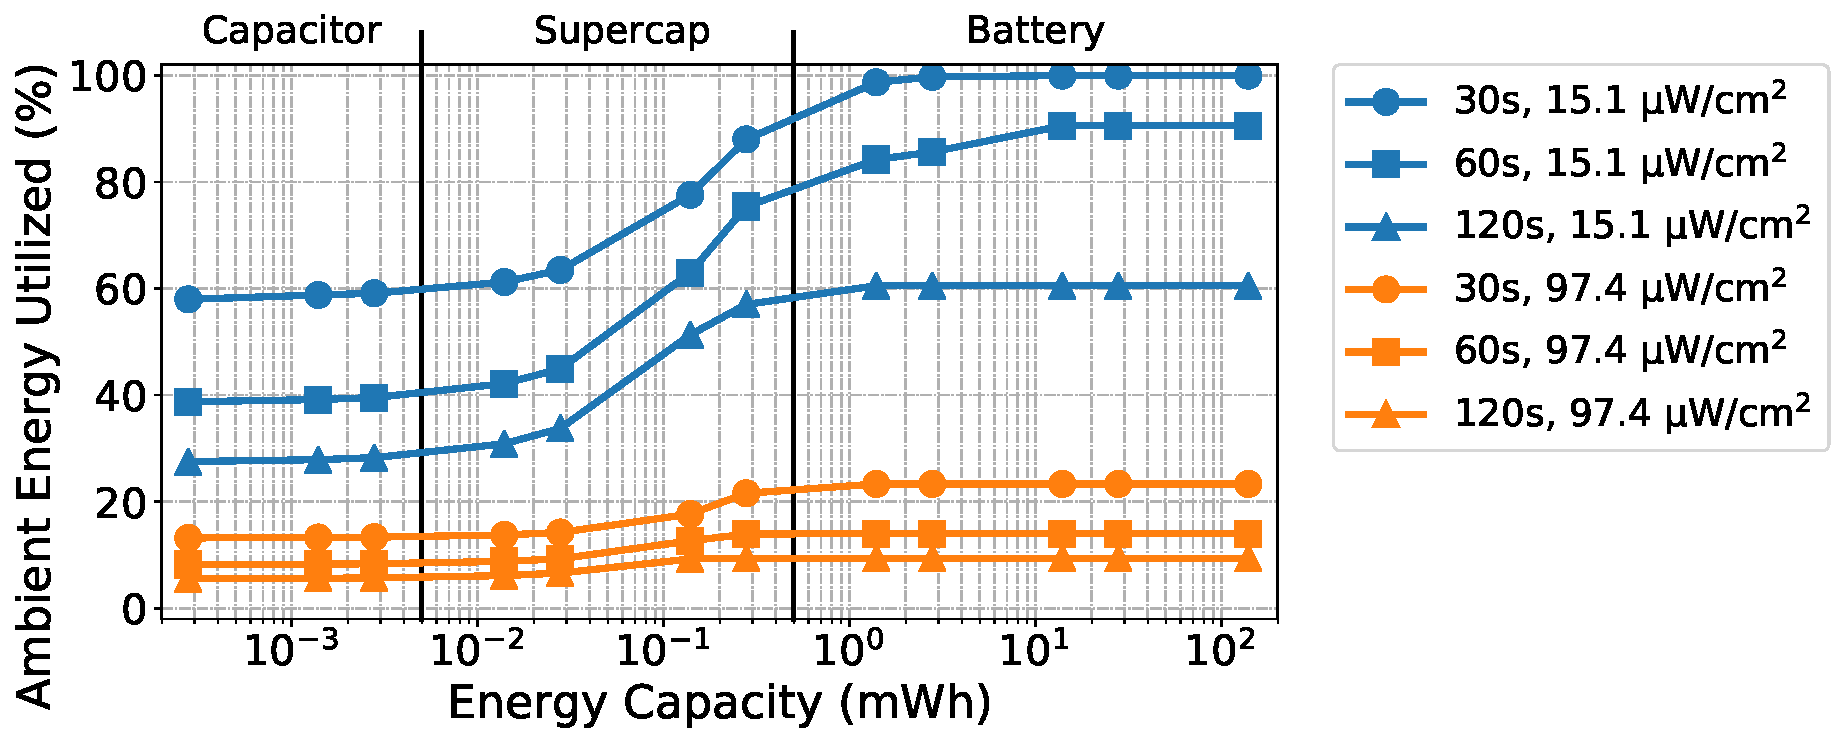
\includegraphics[width=0.9\linewidth]{figs/capacity/sense_and_send/usage_vs_secondary_size}
    \caption{Periodic application}
    \label{fig:usage:sensesec}
  \end{subfigure}
  \begin{subfigure}{0.49\textwidth}
    \centering
    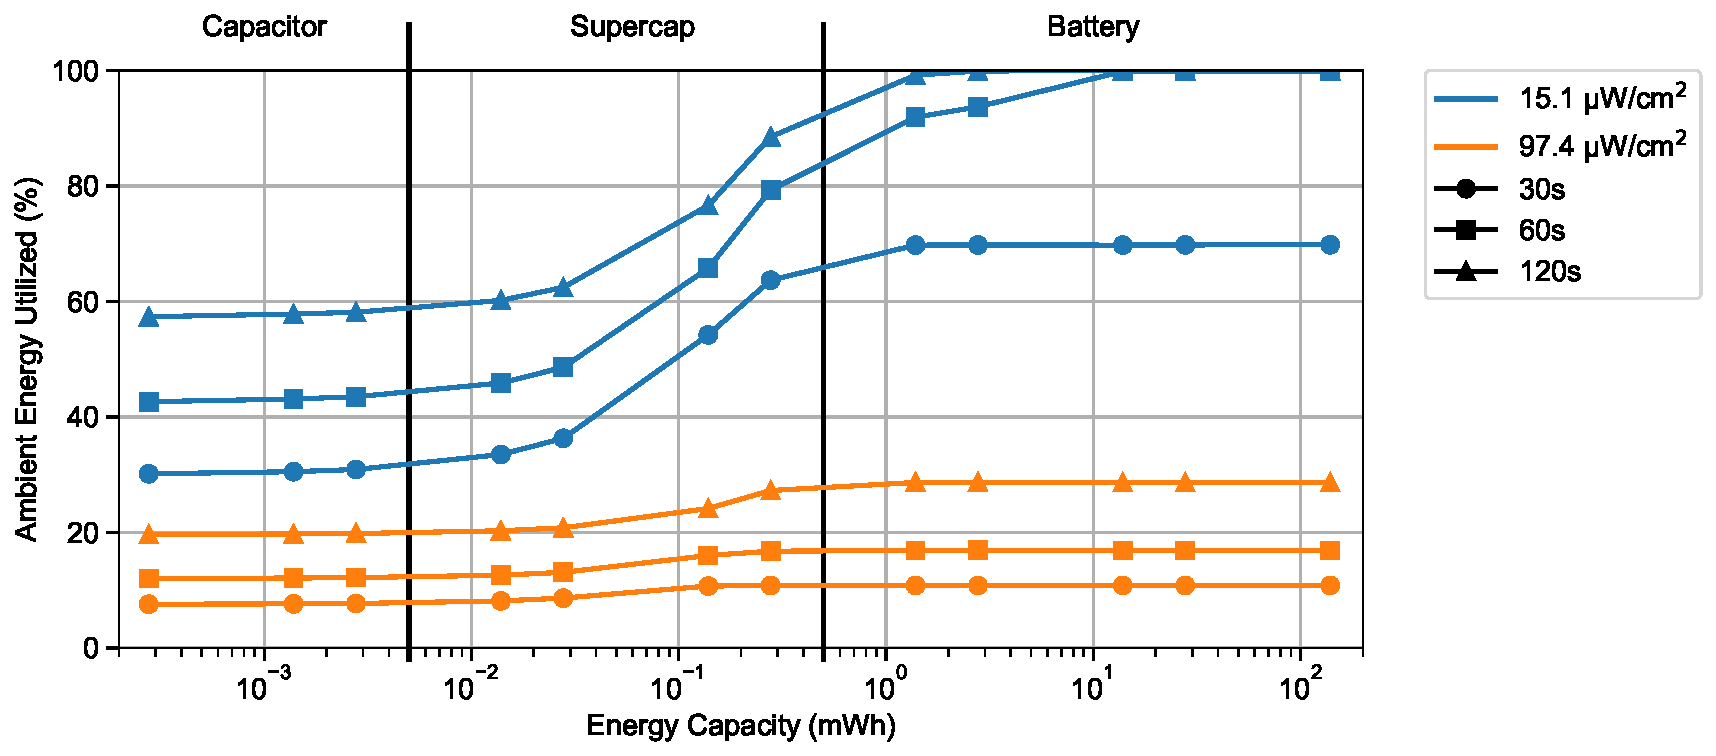
\includegraphics[width=0.9\linewidth]{figs/capacity/door_occupancy/usage_vs_secondary_size}
    \caption{Reactive application}
    \label{fig:usage:eventsec}
  \end{subfigure}
  \caption{\normalfont Ambient energy utilization
    as a function of idealized secondary storage capacity for different
    harvesting scenarios and workloads. The harvesting scenarios and workloads
    are described in \cref{sec:overview} and \cref{tab:capacity:rep}.  The x-axis is
    split by energy capacities possible with capacitors, supercapacitors, and
    batteries. The upper extents of capacity for (super)capacitors represent
    ten 100\,\si{\micro\farad} tantalum capacitors~\cite{tantalumDatasheet}, and one
    large 220\,mF supercapacitor~\cite{murataCap}. Larger capacitors exist, but
    are not appropriate for use on a small sensor node.  As energy storage increases, the harvestable energy used in
    the application also increases, implying
    increased application performance.  Some scenarios, such as the periodic
    30\,s, 15.1\,\uW/cm\textsuperscript{2} case, reach 100\% utilization at
    high secondary capacities indicating that available energy is not
    sufficient to meet the application's requirements.
    Generally, for both workloads and irradiance traces, from
    the smallest to largest capacity simulated, we see a 1.4-2.3x increase in
    utilized energy.
    }
\end{definefigure*}

\begin{definefigure*}{fig:reliability}
  \centering
  \begin{subfigure}{\textwidth}
    \begin{subfigure}{0.5\textwidth}
      \centering
      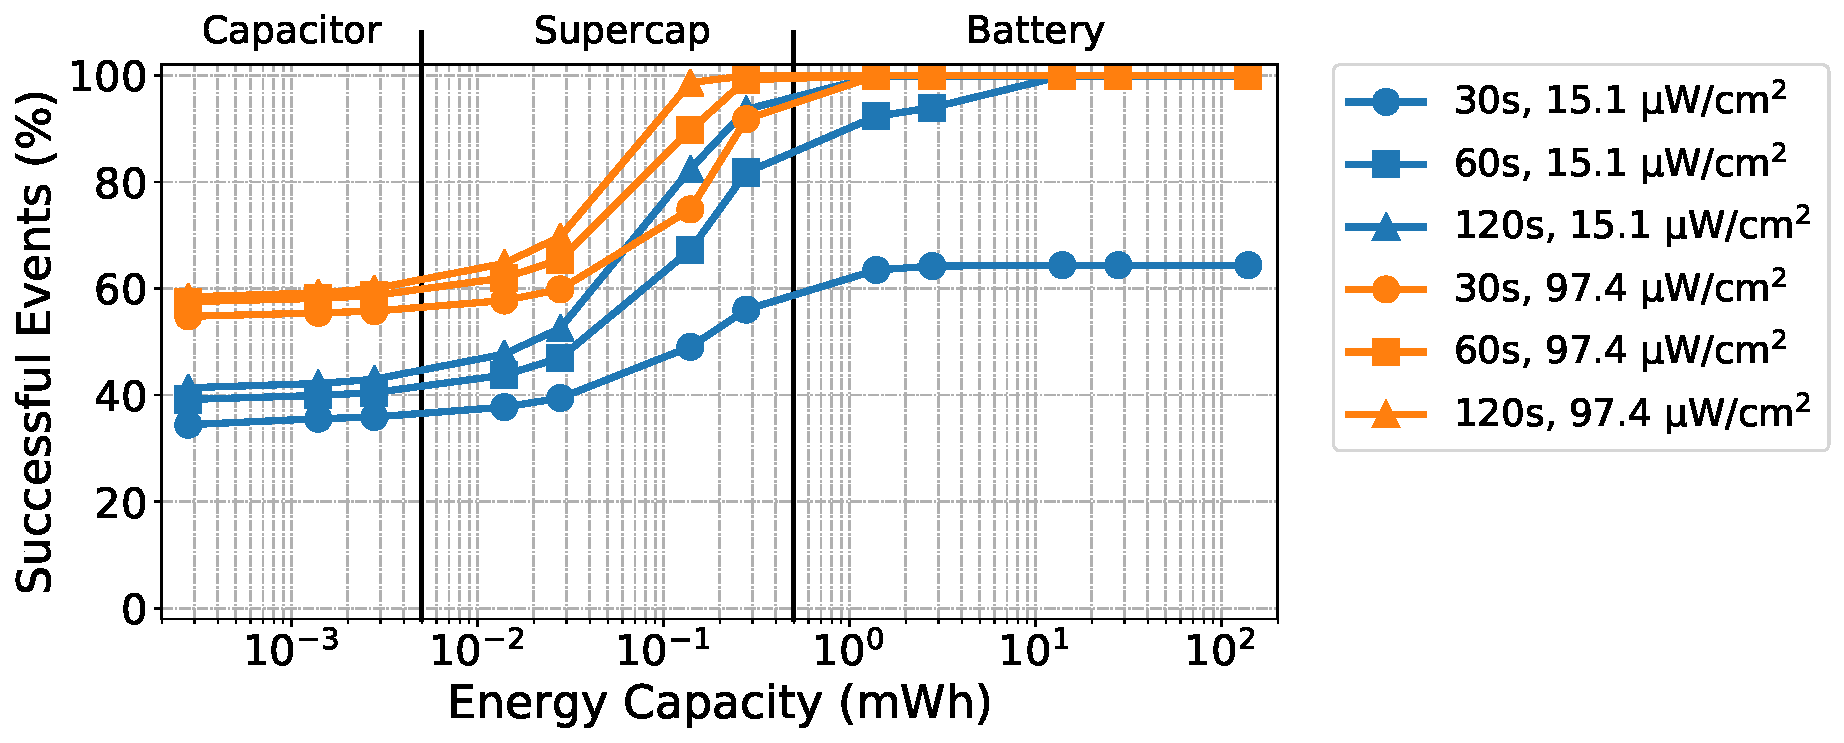
\includegraphics[width=0.9\linewidth]{figs/capacity/sense_and_send/events_vs_secondary_size}
        \caption{Periodic application}
      \label{fig:reliability:sensesec}
    \end{subfigure}
    \begin{subfigure}{0.5\textwidth}
      \centering
      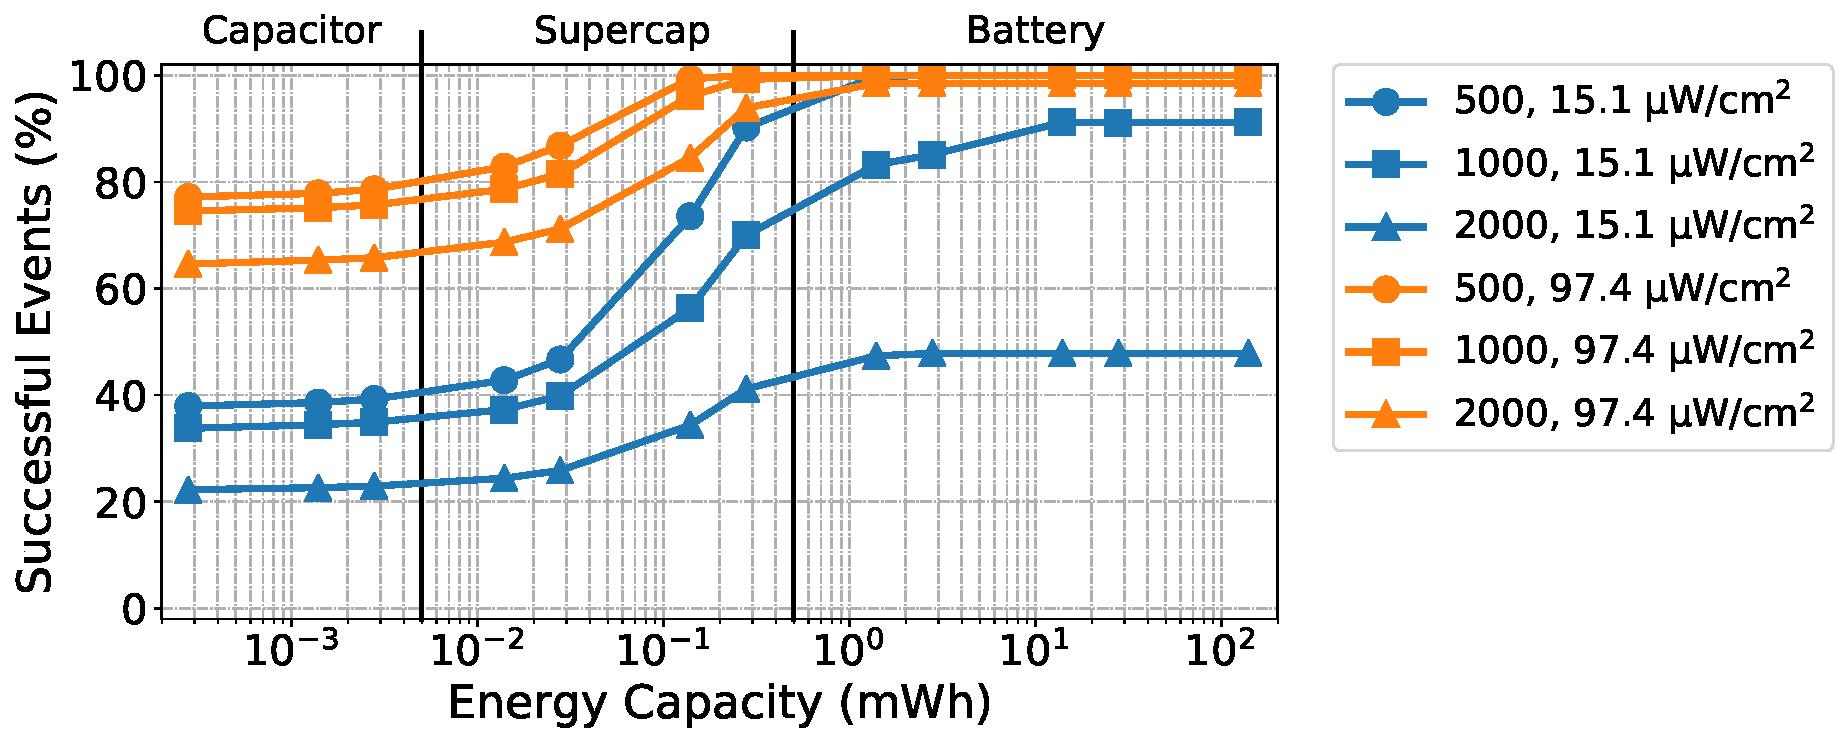
\includegraphics[width=0.9\linewidth]{figs/capacity/door_occupancy/events_vs_secondary_size}
      \caption{Reactive application}
      \label{fig:reliability:eventsec}
    \end{subfigure}
  \end{subfigure}
  \begin{subfigure}{\textwidth}
    \begin{subfigure}{0.5\textwidth}
      \centering
      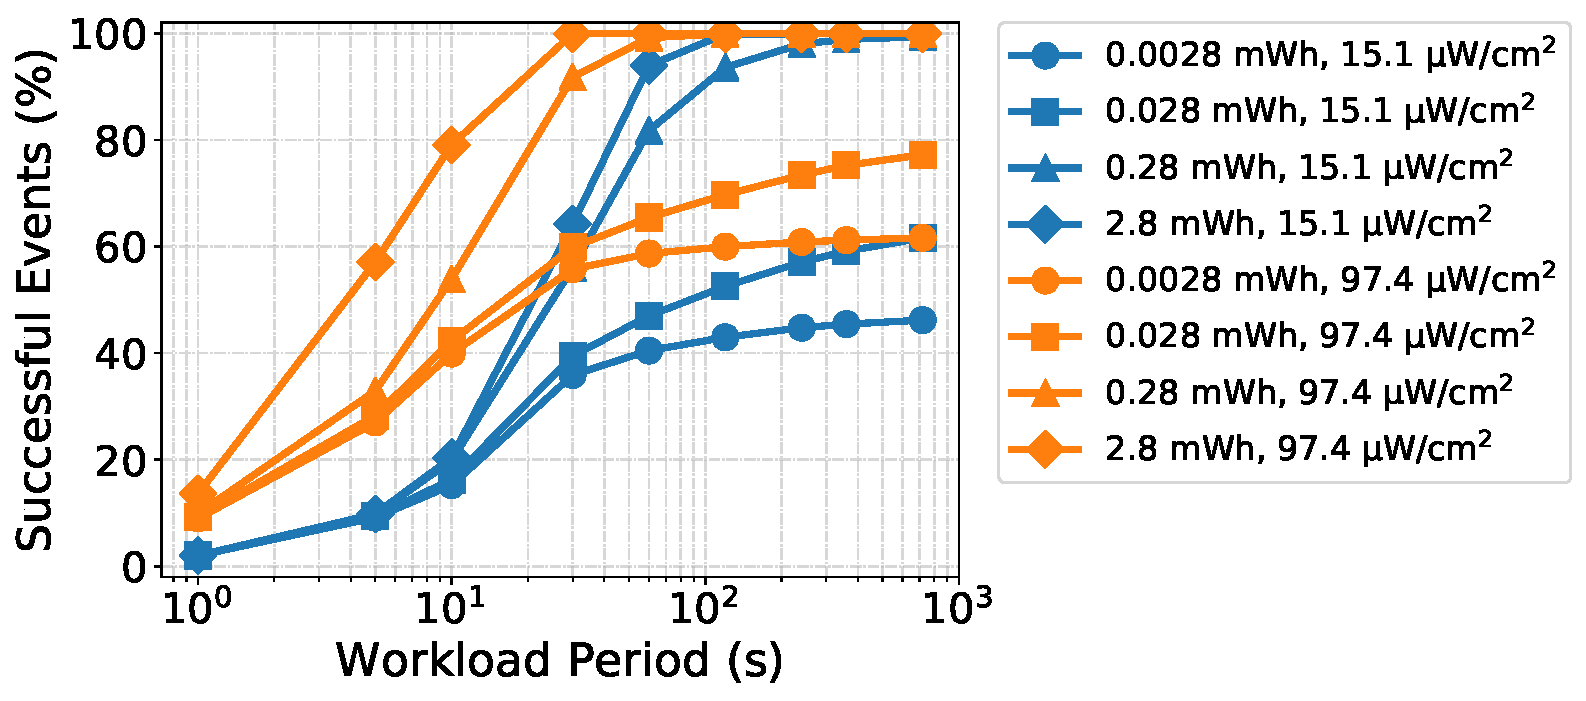
\includegraphics[width=0.9\linewidth]{figs/capacity/sense_and_send/events_vs_period}
      \caption{Periodic\textemdash varying period}
      \label{fig:reliability:senseper}
    \end{subfigure}
    \begin{subfigure}{0.5\textwidth}
      \centering
      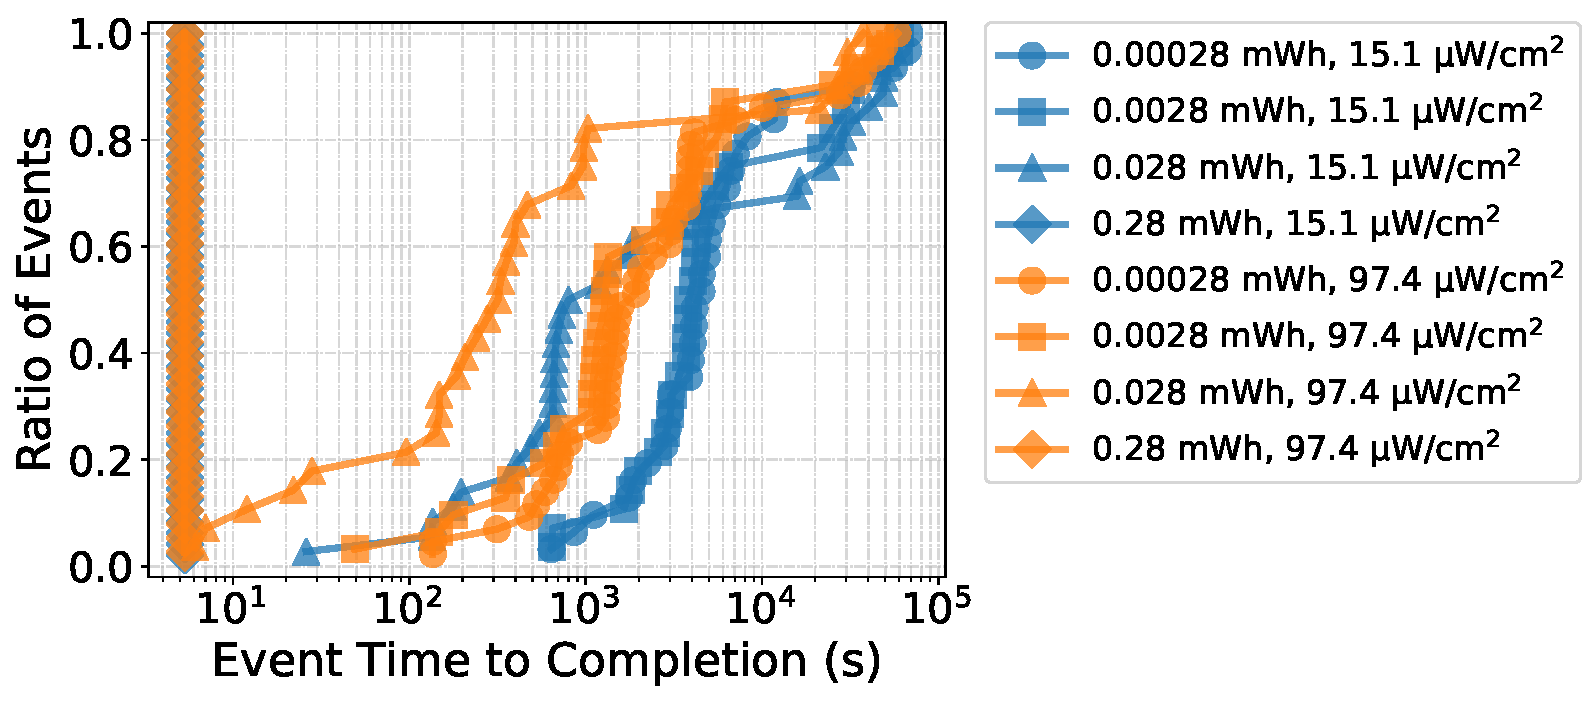
\includegraphics[width=0.9\linewidth]{figs/capacity/ota_update/ttc_ota}
      \caption{Long-running, high energy event}
      \label{fig:reliability:otattc}
    \end{subfigure}
  \end{subfigure}
  \caption{
    \normalfont
    Workload reliability
    for different harvesting scenarios, workloads, and idealized secondary storage sizes.
    We define reliability as the percentage of successfully completed events.
    As expected,
    workload reliability follows the same
    trend as energy utilization, improving with increased secondary energy
    storage. For both periodic and reactive workloads, from the smallest to
    largest capacity simulated, we see a 1.4-2.7x improvement in availability.
    In (c) we investigate the period at which different secondary storage sizes
    meet a specific reliability, showing that even with infrequent periodic
    workloads, small amounts of secondary storage have low reliability while
    larger secondary stores reach near 100\% reliability. (d) shows a CDF of
    time to completion for events in the long-running workload. In this
    workload, events are not atomic, and can be paused and resumed based on
    available energy. With secondary capacities that are large relative to the
    workload (which takes 93\,mJ) we see immediate completion.
    However, performing the event on smaller secondary capacities can take
    between three hours and a day to complete even for scenarios with large
    amounts of harvestable ambient energy.
    }
\end{definefigure*}

\begin{definetable}{tab:capacity:rep}
    \begin{threeparttable}
    \centering
    \scriptsize
    \begin{subtable}{\columnwidth}
            \centering
            \scriptsize
            \begin{tabular}{r | c | c | c | c }
                \parbox{1cm}{\raggedleft Irradiance\\Trace} & Total Days & \parbox{1cm}{\centering Average\\Power\\(\textmu W/cm\textsuperscript{2})} & \parbox{1.6cm}{\centering 90\textsuperscript{th} Percentile\\Daily Power (\textmu W/cm\textsuperscript{2})} & \parbox{1.6cm}{\centering 10\textsuperscript{th} Percentile\\Daily Power (\textmu W/cm\textsuperscript{2})} \\\hline
                EnHANTS A   & 394  & 15.1     & 25.0      & 5.2\\
                EnHANTS D   & 311  & 97.4     & 256.5     & 24.8\\
                %Enhants C   & 327  & 745.4    & 1610.0    & 176.1\\
            \end{tabular}
            \caption{Indoor photovoltaic irradiance traces}
        \end{subtable}\\
        \vspace{-6pt}
        \begin{subtable}{\columnwidth}
            \centering
            \scriptsize
            \begin{tabular}{r | c | c | c}
                Workload Class & Energy per Event (uJ) & Average Period & Average Power (\textmu W)\,\tnote{a}\\\hline
            \multirow{4}{*}{Periodic}   & \multirow{4}{*}{586}  & 10\,s                 &  58.6     \\
                                        &                       & 30\,s                 &  24.5     \\
                                        &                       & 60\,s                 &  14.7     \\
                                        &                       & 120\,s                &  9.8      \\\hline
            \multirow{3}{*}{Reactive}   & \multirow{3}{*}{86}   & 3.4\,s\,\tnote{b}     &  25.3     \\
                                        &                       & 6.8\,s\,\tnote{b}     &  17.6     \\
                                        &                       & 13.6\,s\,\tnote{b}    &  11.3     \\\hline
                 Long-Running           & 93,300                 & 2\,weeks\,\tnote{c}  &  5.1      \\
            \end{tabular}
            \caption{Representative workloads}
        \end{subtable}
    \end{threeparttable}
    \vspace{-4pt}
    \begin{tablenotes}[para]
    \scriptsize
    \item[a] Average power includes an average 5\,\textmu W idle power, measured in \cref{sec:impl:permamote}.\\
    \item[b] Event times are based on a Poisson distribution for each hour of the day and drawn every second. The distribution is parameterized by collected entryway data then scaled.\\
    \item[c] Event time is based on a uniform distribution and drawn every second.
    \end{tablenotes}
    \caption{\normalfont Representative harvesting conditions and workloads.
    To evaluate different energy storage architectures, we define a set of energy harvesting
    conditions and workloads that are representative of common sensing applications. We choose two
    real, 1\,Hz, irradiance traces with different magnitudes of available energy. We define three
    workloads: periodic, reactive, and long-running, and we characterize those workloads
    for different event frequencies. The energy used for each event is measured
    on our reference hardware described in \cref{sec:impl:permamote}.
    }
\end{definetable}

\begin{definetable}{tab:parameters}
    \centering
    \begin{adjustbox}{width=\columnwidth}
    \begin{tabular}{lll}
\hline
\textbf{Config Type}& \multicolumn{1}{l}{\textbf{Parameter}}                   & \multicolumn{1}{l}{\textbf{Description}} \\ \hline
\textbf{Device}     & \texttt{operating\_voltage}                              & Output voltage of the power subsystem    \\
                    & \texttt{boost\_efficiency}                               & Efficiency of the boost converter        \\
                    & \texttt{frontend\_efficiency}                            & Efficiency of the harvesting frontend    \\ \hline
\textbf{Secondary}  & \texttt{capacity}                                        & Capacity of secondary in joules or mAh   \\
                    & \texttt{esr}                                             & Equivalent series resistance in ohms     \\
                    & \texttt{leakage\_constant}                               & Factor for capacity dependent leakage    \\
                    & \texttt{\string{max, min\string}\_hyst}                  & Secondary capacity upper/lower hysteresis\\ \hline
\textbf{Primary}    & \texttt{capacity}                                        & Capacity of primary in mAh               \\
                    & \texttt{leakage\_percent}                                & Percent capacity leakage per year        \\ \hline
        \textbf{Harvester}  & \texttt{area}                                    & Area of solar harvester in cm\textsuperscript{2}\\
\textbf{(Solar)}    & \texttt{efficiency}                                      & Efficiency of solar panel                \\ \hline
%\textbf{Workload}   & \texttt{type}                                            & Periodic or Reactive                     \\
%                    & \texttt{period/scale}                                    & Period, or scale for average \# of events \\
%                    & \texttt{opportunistic}                                   & Ignore period, and perform events ASAP   \\
%                    & \texttt{sleep\_current}                                  & Current draw of system in low power mode \\
%                    & \texttt{startup\_\string{energy, period\string}}         & Energy, time required for startup        \\
%                    & \texttt{event\_\string{energy, period\string}}           & Total energy, time required for work event \\
%                    & \texttt{atomic}                                          & Workload is atomic, or intermittent      \\
%                    & \texttt{event\_period\_min}                              & If not atomic, minimum splitable period  \\ \hline

    \end{tabular}
    \end{adjustbox}
    \caption{\normalfont Simulation configuration parameters.
      A representative set of available configuration options for our
      simulation of a sensor with secondary storage and energy harvester, a
      primary-cell, or both. A secondary-cell can be configured with a
      hysteresis, with a lower bound set to \texttt{min\_hyst}
      and an upper bound of \texttt{max\_hyst}.
      %This upper bound must represent
      %the minimum amount of
      %energy to do useful work.
      %Therefore, the upper bound of charging
      %hysteresis is set to \texttt{secondary\_max\_hyst}.
      %Workloads are
      %configured to be either periodic or reactive, and workload intensity is
      %determined by period, or a scaling factor determining the average number
      %of events picked from a random distribution.
      }
\end{definetable}
\begin{definefigure}{fig:statemachine}
    \centering
    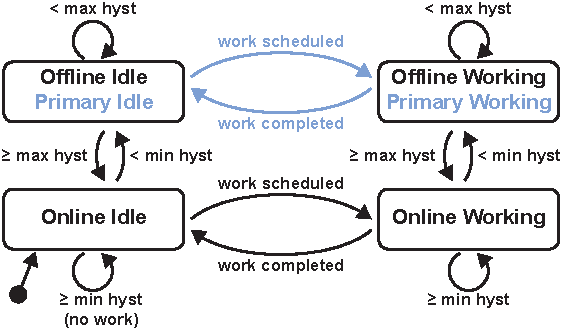
\includegraphics[width=\columnwidth]{figs/capacity/model_state_machine}
    \caption{\normalfont Model state machine.
    A modeled device can be in one of four states: \textsf{Offline Idle},
    \textsf{Online Idle}, \textsf{Online Working}, and \textsf{Offline
    Working}. When a device is \textsf{Offline Idle}, it has run out of energy
    and is off. If a device is \textsf{Online
    Idle}, it is on and in deep sleep, ready to perform work if triggered. If
    triggered, a device moves to \textsf{Online Working}, where it performs a
    portion of a work event.  If a workload is atomic, workload events
    \textit{must} be completed in one \textsf{Online Working} step, without any
    transitions to an offline state.  \textsf{Offline Working} means that while
    working on a non-atomic task, the device ran out of energy, checkpointed,
    and is waiting to harvest more and resume its task.  For devices
    configured with a primary-cell, \textsf{Offline Idle} and \textsf{Offline
    Working} become \textsf{\textcolor{primary-blue}{Primary Idle}} and
    \textsf{\textcolor{primary-blue}{Primary Working}} respectively.  In these
    states, outgoing energy is charged against the primary-cell and the device
    remains online and able to perform work for the life of the primary-cell.
    %State transitions are determined by incoming energy, the state of charge of
    %the secondary storage, and the generated work schedule from workload
    %parameters.
    }
\end{definefigure}

\section{\name Implementation}
\label{sec:impl:permamote}

%We discuss the implementation of both the model used to generate the results
%of \cref{sec:store} and \cref{sec:primary}, and the \name hardware that
%is based on these results. All of our hardware and software will be made
%\textbf{open source} for use by other researchers.


\begin{definetable}{tab:components}
    \begin{threeparttable}
    \centering
    \scriptsize
        \centering
        \scriptsize
        \begin{tabular}{l | l | c | c}
            Component                           &  Function                     & Active Power          & Idle Power \\\hline
            \multirow{2}{*}{Nordic NRF52840}    & Processor                     & 56\,\uA/MHz           & 940\,nA\,\tnote{a}  \\
                                                & Radio                         & 5.2\,mA @ 0\,dbm      & \textemdash\,\tnote{a}\\
            Ambiq AB1815-T3                     & Real time clock               & 55\,nA                & N/A\,\tnote{b}  \\
            ST Micro LIS2DW12                   & Accelerometer                 & 1\,uA @ 12.5\,Hz      & 50\,nA  \\
            Maxim MAX44009                      & Light sensor                  & 650\,nA               & N/A\,\tnote{b}  \\
            Intersil ISL29125                   & Color sensor                  & 56\,\uA               & 500\,nA  \\
            Silicon Labs SI7021                 & Humidty sensor& 1.5\,\uA @ 1\,Hz      & 60\,nA  \\
            TE Connectivity MS5637              & Pressure sensor               & 0.6 - 5\,\uA @ 1\,Hz  & 10\,nA  \\
            Panasonic EKMB11011                 & PIR Occupancy                 & 100\,\uA              & 1\,uA  \\
        \end{tabular}
    \end{threeparttable}
    \begin{tablenotes}[para]
    \scriptsize
    \item[a] Sleep current for both processor and radio.
    \item[b] No shutdown or idle mode.
    \end{tablenotes}
    \caption{
    \normalfont
    The components used in \name.
    These components are among the lowest power options available, and
    are even 2-4x lower power than those used on relatively recent
    systems such as BLEES, Flicker, Capybara, and Hamilton.
    }
    %Technology
    %scaling for embedded sensors, processors, and radios
    %has driven down the average power of a sensor node much closer to the
    %harvestable solar energy available in indoor lighting conditions. This allows
    %more systems to subsist or achieve extended lifetimes through energy harvesting.
\end{definetable}

\begin{definefigure}{fig:permamote}
    \centering
    \begin{subfigure}{0.7\columnwidth}
        \centering
        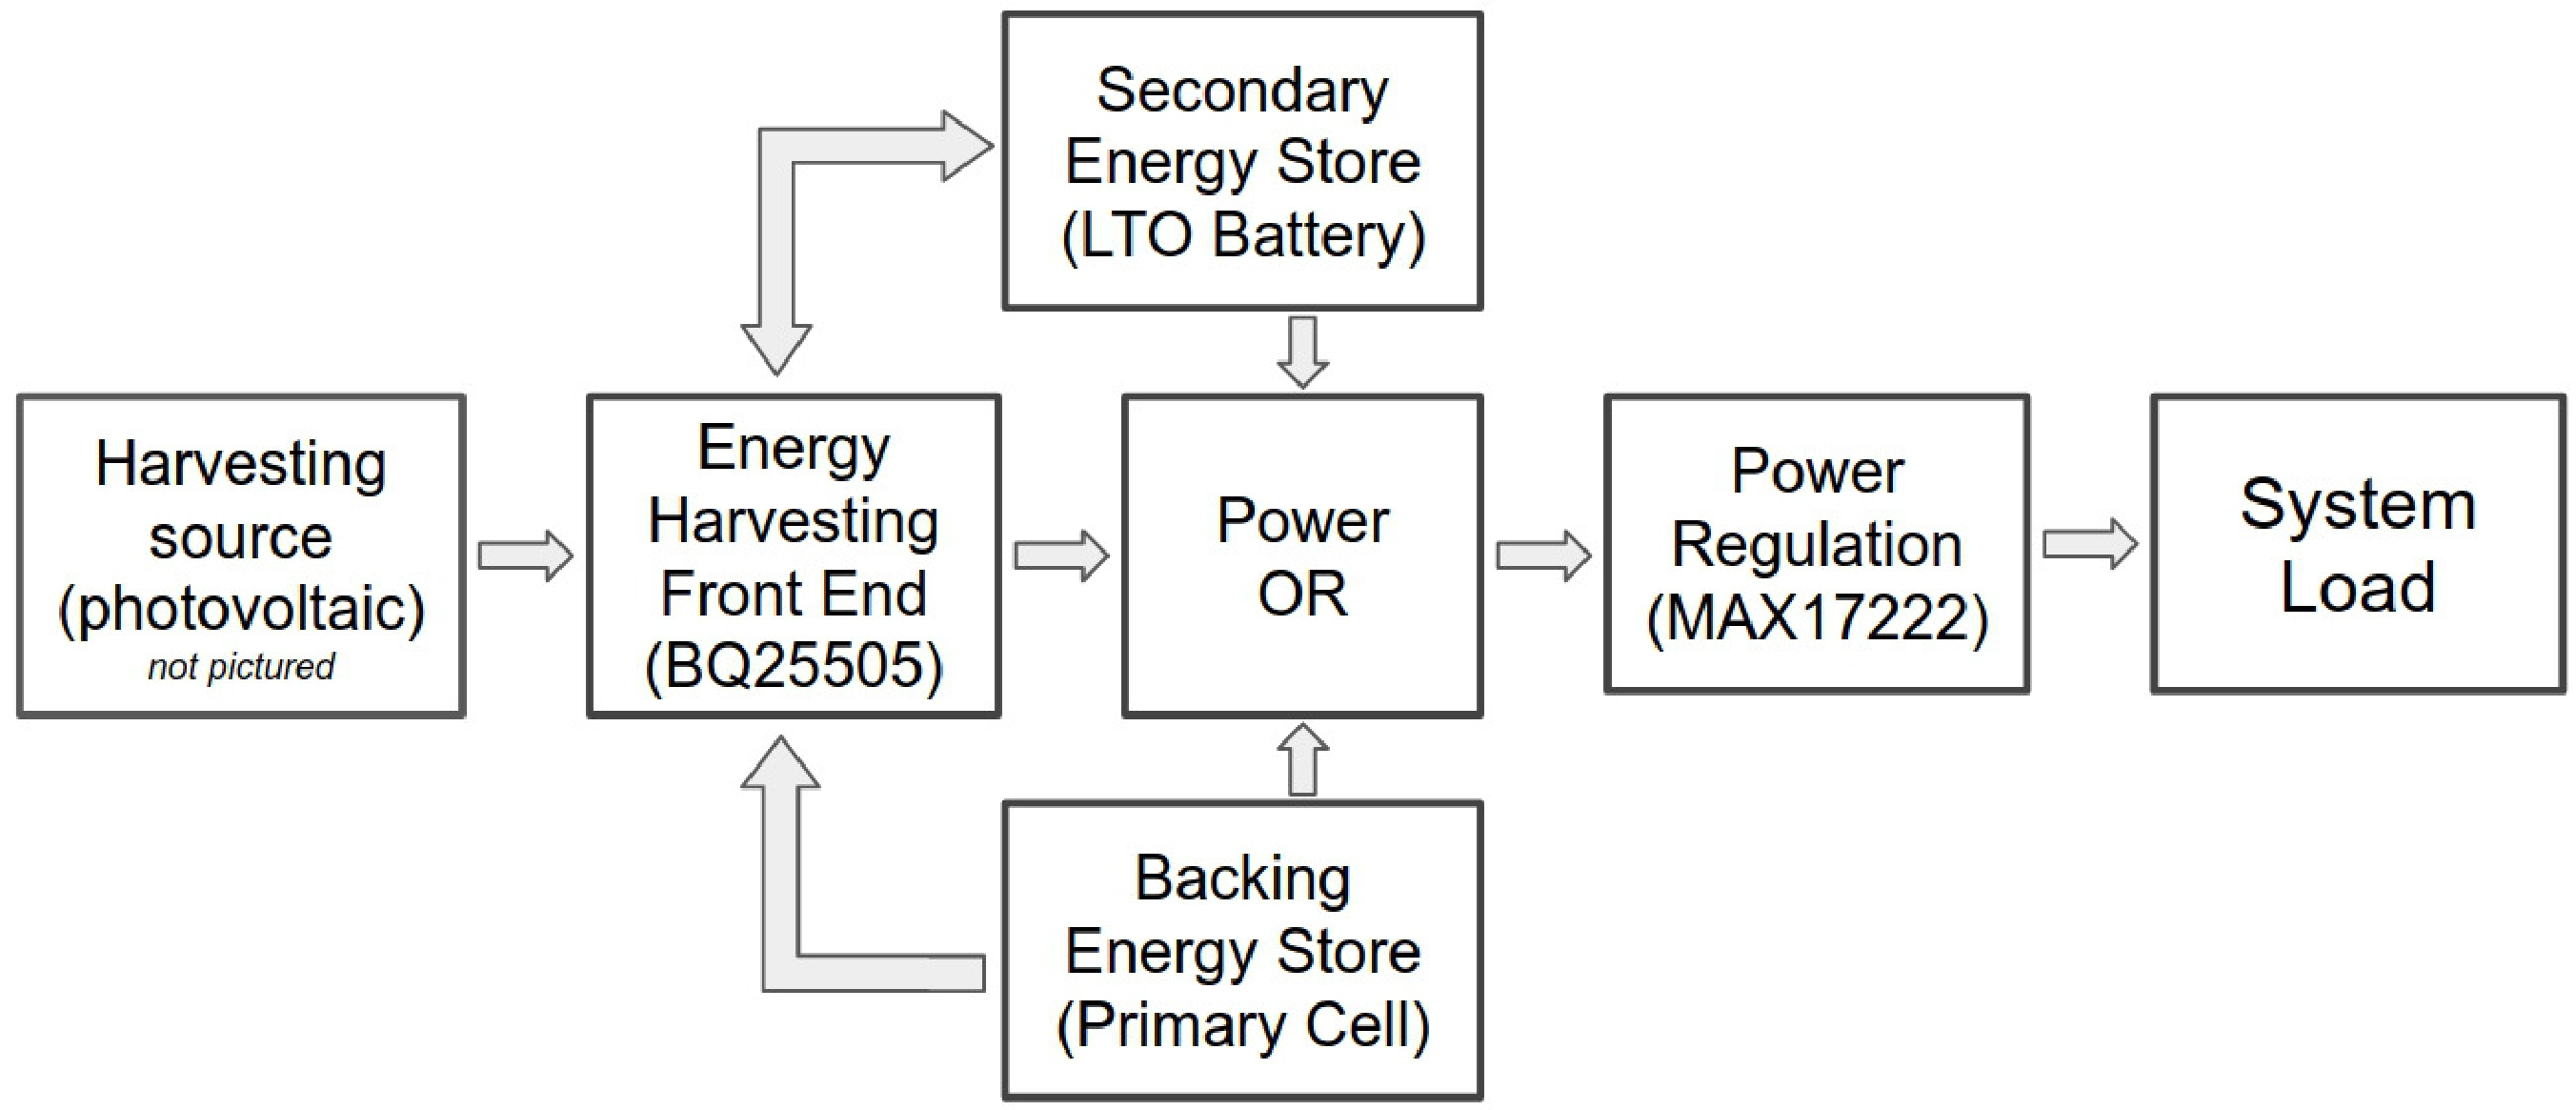
\includegraphics[width=\textwidth]{figs/capacity/arch}
        \caption{Harvesting and storage architecture}
    \end{subfigure}
    \begin{subfigure}{0.29\columnwidth}
        \centering
        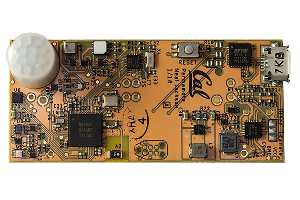
\includegraphics[width=\textwidth,angle=90]{figs/capacity/permamote}
        \caption{Hardware}
    \end{subfigure}
    \caption{\normalfont The \name power supply architecture is informed by the
    findings in \cref{sec:store,sec:primary}. An
    LTO battery is recharged by a solar panel. When the battery is depleted,
    a primary-cell powers the system, providing reliability and avoiding
    intermittency.
    }
    %We believe this platform will run for 6-36 years for common
    %sensing tasks and indoor lighting conditions before the death of
    %the primary-cell. Even after the primary-cell expires,
    %the sensor node could continue to run intermittently on harvested energy.
\end{definefigure}

We implement the design principals discussed in \cref{sec:store,sec:primary}
in a new sensor called \name. The \name sensing platform
integrates a processor, BLE/802.15.4 radio, and various environmental, lighting,
and occupancy sensors. A picture
and system diagram of \name is shown in \cref{fig:permamote}. All hardware
and software for the platform is open source\footnote{\url{https://github.com/lab11/permamote/tree/master/hardware/permamote}}.\\

\vspace{-6pt}
\noindent
\textbf{Energy Harvesting and Storage.}
\name is powered by an energy harvesting front end that realizes the benefits
of using batteries. It uses the TI BQ25505 energy harvesting IC, which
harvests energy while monitoring both
rechargeable and backup energy stores,
switching between them at user-configurable voltages~\cite{bq25505}. A
20\,mAh (48\,mWh) LTO battery is charged by an 10.9\,cm\textsuperscript{2} amorphous
silicon solar panel~\cite{LTODatasheet, LTODatasheet2}. We limit the apparent
capacity of this battery to ensure
longer cycle lifetime as described in \cref{sec:battery}, but still have 24\,mWh of
energy storage, more than the capacity required to achieve the reliability and energy utilization
improvements described in \cref{sec:store}. For the backup energy
store, \name uses lithium primary-cells which can be configured to either one or two CR2032 coin
cells or a CR123A cell.
%Primary-cells provide 3-13x more density and 2-12x less
%leakage than a secondary-cell.
%making them more desirable than a single,
%large, pre-charged secondary-cell as the backup store~\cite{LTODatasheet,primary2032, primarycr123a}.
The output of the active battery
is boosted by a MAX17222 regulator, which features high conversion efficiency
(>90\%) at low output currents and operates down to 400\,mV~\cite{max17222}.\\
%We have the ability to monitor harvesting and system currents using
%the iCount method by sensing the voltage of
%the inductor used by the BQ25505 and MAX17222~\cite{duttaEnergy08}. The processor
%is also capable of gating all sensors from the main power supply to save
%power.\\

\vspace{-6pt}
\noindent
\textbf{Processor, Radio and Sensor Selection.}
In designing \name, we search for the newest and lowest power components.
%We feel that it may
To benefit other
platform builders, we document our component selections
along with their key performance metrics. A summary of these
components can be found in \cref{tab:components}.

We note our choice of the Nordic NRF52840 MCU over the more commonly used MSP430FR series
because of its higher efficiency in active mode while offering comparable sleep currents.
Specifically, it only draws 56\,\uA/MHz compared to over 100\,uA/MHz
for the MSP430. Unlike intermittent systems,
we do not rely on the FRAM present on the MSP430FR series chips. While
slightly more efficient
processors and radios exist than those found in the NRF52840,
we value the simplicity of an SoC-based design. \\

\vspace{-6pt}
\noindent
\textbf{Energy Benchmarks}.
The data presented in \cref{tab:components} are benchmarks taken
on the \name platform. We find that a BLE advertisement at 0\,dbm consumes
86\,\uJ and that sampling both light and color sensors and transmitting
them in a BLE advertisement consumes 586\,\uJ. Additionally, the entire system, including
the energy harvesting front end, consumes only 5.0\,\uW in deep sleep with RAM
retained and all sensors powered off. We use the energy numbers from \name as a basis
for our workloads to fairly compare against prior energy storage architectures.
%\subsection{Numerical Model}
%\label{impl:model}
%
%We develop a numerical model that simulates the behavior of energy harvesting
%systems in indoor environments. For this work, we've primarily focused on solar
%energy input, and have tailored the model to use solar energy traces. As
%mentioned, we use the Columbia EnHANTs irradiance traces
%\cite{margolies2015energy}. We process the traces, filling the few periods of
%missing data by copying from a week prior.
%
%The model operates at second granularity, and at each
%step, the amount of incoming energy is calculated based on the input irradiance
%and solar panel configuration. If the device has enough energy to turn on
%and perform the task from the specified workload it does so. If there is
%energy to spare after the task, the device will enter a low power sleep state.
%The model tallies the amount of successful and unsuccessful events that it
%was expected to complete, as well as the percentage of energy used out
%the energy that was available from the harvesting source. To estimate
%lifetime, the model attempts tasks for the totality of solar irradiance
%data present, then extrapolates primary-cell discharge to find its lifetime
%at empty. The one second granularity imposes some limitations, however
%we find that sensor node workloads are rarely more intensive.
%
%If the secondary store is not at capacity
%this incoming energy is stored
%
%If the device is online, it attempts to turn on
%if it has enough energy to do so, otherwise it remains offline and continues to
%fail performing its workload.  If the device is on, it perform tasks from its
%workload. It prioritizes using the energy from its rechargeable store, and if
%depleted, will either go offline or use energy from its primary-cell, if
%available. If it has energy to spare, it enters a low power sleep state. The
%model tallies the amount of successful and unsuccessful events that it was
%expected to complete, as well as the percentage of energy it used out of how
%much was available from the irradiance source. It also performs a linear fit on
%the primary state of charge to estimate lifetime, if applicable to the
%simulated device's configuration.
%
%This
%granularity also limits that of workloads to a second, but we argue
%that realistic sensor workloads are rarely more intensive \hl{cite}.


\placefigure[t]{fig:permamote}


\section{Model Evaluation}
\label{sec:eval}
To evaluate the model, we perform a three-month-long deployment in a partially sunlit room
using i) a primary-cell only system, ii) an intermittent, capacitor-only system, and iii) \name, our
system that features both a secondary and primary-cell. We model these
systems over the same period and compare the availability of \name to the
intermittent system.

\subsection{Model Analysis}
\label{sec:eval:model}
We analyze the deployment of these systems
%in a partially sunlit room for three months
and compare their behavior to our
model's predictions: i) ten CR2032 primary-cell only devices, ii) an
intermittent system configured with just 500\textmu F of capacitance (about
0.36\,\textmu Wh at 2.2\,V), and iii) \name, configured with a 20\,mAh
(48\,mWh) secondary-cell, half of which is usable, and a CR2032 backup.  The
primary-cell only device performs environmental sensing over BLE every second.
The intermittent system  sends a beacon as soon as its capacitor bank is full.
When its energy is depleted, it powers off and charges
again. \name is running the ``sense and send'' workload that we described in
\cref{sec:overview}, and sends illuminance measurements every second. This
workload stresses the model and requires more charge and discharge cycles.  We
use \name illuminance readings to estimate irradiance using the same scaling factors used by
Yerva et al.~\cite{yervaGrafting12}, and use these traces as
model input.\\

\vspace{-6pt}
\noindent
\textbf{Primary-Cell Only.}
We model the workload of the primary-cell system and produce estimates for
lifetime.  Our model predicts the platform lifetime
to be 58 days.  We find that the average lifetime of the 10 devices is 61 days.
%,
%from initial deployment to energy depletion, is 61 days.
\\

\vspace{-6pt}
\noindent
\textbf{Intermittent.}
We model the number of packets sent each hour by the
intermittent system over a three week period, and compare against the results of an actual device in
\cref{fig:eval:pkt}.
The average daily error of the model versus our results is 15\%, with a standard deviation of
17\%. This error can attributed to two primary sources. Illuminance is measured
close to, but not exactly at the solar panel of the test device. Occasional
direct sunbeams, like that experienced on day 16, can illuminate the solar
panel but not the sensor, or vice versa. This
results in a substantial over or underestimate of available light. In addition
to inaccurate light measurements, we introduce error through our estimation of
irradiance. We measure illuminance
instead of irradiance, and must resort to a piecewise linear estimation, when
in reality the relationship is not well defined and non-linear when considering
different light sources. In the case of our estimation, results
indicate that the model consistently underestimates high irradiance measurements.\\
\placefigure{tab:components}
\placefigure[t]{fig:evalcmp}

\vspace{-6pt}
\noindent
\textbf{Secondary and Primary-Cell.}
We compare our model's predicted state of charge to a deployed \name over a seven
day period in \cref{fig:eval:soc}. We estimate state of charge from the reported secondary-cell
voltage,
%,
%and measured voltage
%curves of the installed 20\,mAh battery
and irradiance from
lux measurements. In this figure, the state of
charge cycles between configured battery hysteresis limits, as the workload is
too intense to be sustained by energy harvesting alone.
%and the Permamote must
%use energy from its primary cell.
Flat and upward slopes of the curve represent the
device in hysteresis, using the primary battery to perform its workload. Upper slopes
indicate the secondary cell is charging from harvested energy.
Downward slopes indicate the device is out of hysteresis and is using harvested
energy stored in its secondary battery to perform its workload.
%The device is
%charging and in
%hysteresis during upward
%slopes.
The shaded ``nighttime'' regions are not uniform, as the
deployment environment is occupied by graduate students that occasionally work
late hours or forget to turn off the lights.  The model correctly predicts the
cycling
behavior of the deployed device for two days, but deviates
during the third day. The model predicts that the device would charge above the upper
hysteresis limit and begin supplying energy from the secondary-cell before the
test device actually does.  This inaccuracy, like that of the last of
experiment, is partially due to our inexact estimation of irradiance.  In
addition, real device hysteresis limits are set using resistor networks.  The
resistors used have 1-5\% tolerance, and are susceptible to temperature
changes, which introduces dynamic errors that is not accounted for in our model.
Even though the predicted state of charge deviates after two days, the length
and frequency of periods in which harvested energy is stored and used %in the secondary-cell
are identical to our experimental measurements.
%While our model correctly predicts cycling timing and frequency, it appears the
%state of charge  does not quite match that of the measurements.  This is
%because the voltage measured is not the open circuit voltage, and is affected
%by voltage droop due to the applied system load as well as inflated charging
%voltage from the energy harvesting front end.  Ignoring these effects, the
%cycling of the model's prediction is closely synchronized with the estimated
%state of charge.
%We compare the model's predicted
%state of charge over time to the outputs of systems we
%have deployed. For energy harvesting systems we collect lux measurements
%throughout the deployment and convert lux to irradiance based on the
%data collected in Yerva et al.~\cite{yervaGrafting12}. \\
%\vspace{-6pt}
%\noindent
%\textbf{Permamote.}\\
\subsection{\name Performance}
\placefigure[t]{fig:eval}
\label{sec:eval:permamote}
%In addition to evaluating our model,
We also compare the performance of the
deployed intermittent system and \name. In \cref{fig:evalcmp}, we show the
number of packets sent per hour for two days. \name sends data every
second, while the intermittent system sends as fast as possible. \name is
able to collect and send its data continuously, while the
intermittent system is limited to sending only during the day. This
demonstrates the increased availability afforded by increasing secondary
capacity and including a backup energy store.

We also use our model to explore the estimated performance of \name
compared to prior systems.
To isolate the analysis to just power supply types and sizing, we assume each
system uses the same low-power hardware and is performing the same workload.
The results of this modeling are shown in \cref{tab:related}. Our model estimates that
\name can expect several decades of 100\% reliable lifetime when configured as
it was deployed for this evaluation, albeit configured with a less intense workload.
%While the workload used with \name is not
%sustainable for the multi-decade lifetimes we are targeting, it still
%exemplifies the increase in reliability afforded by including a primary-cell.


\begin{definefigure}{fig:eval}
  \centering
  \begin{subfigure}{\columnwidth}
    \centering
    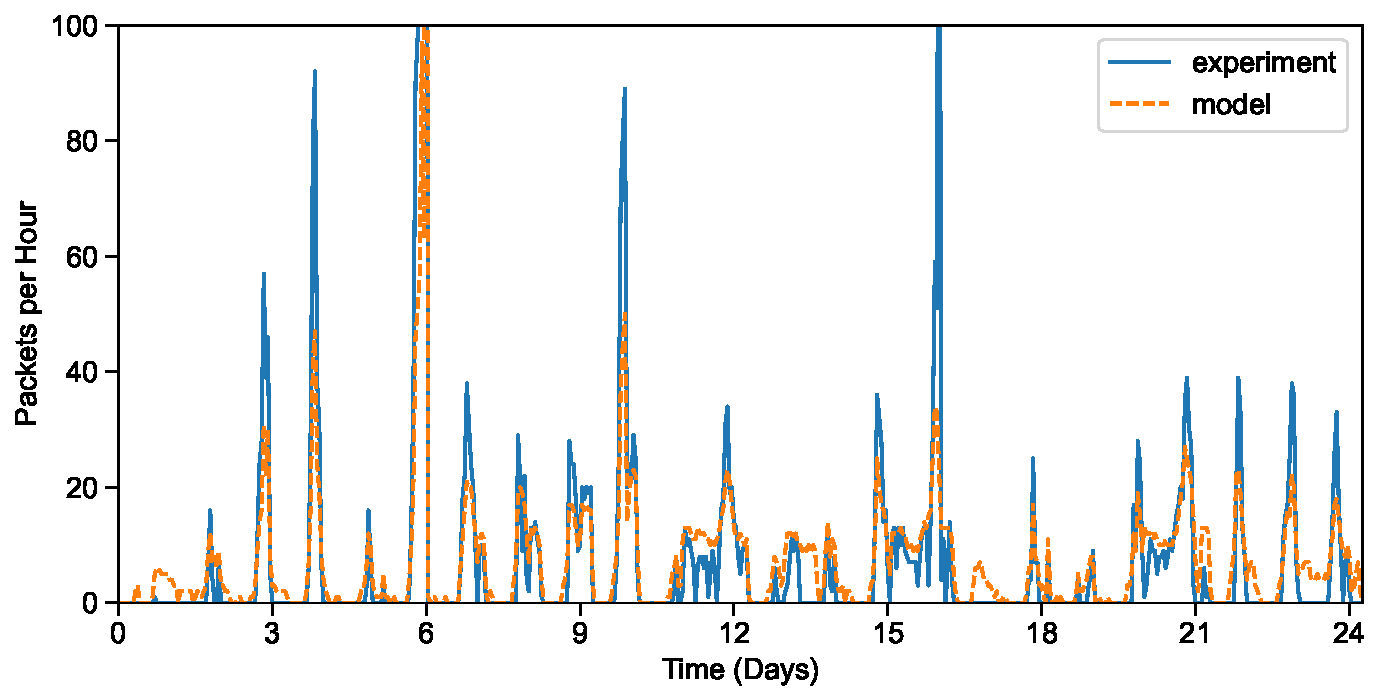
\includegraphics[width=\linewidth]{figs/capacity/experiment_pkt/exp_vs_sim_pkt}
    \caption{Intermittent Node}
    \label{fig:eval:pkt}
  \end{subfigure}\\%\hspace{0.5cm}
  \begin{subfigure}{\columnwidth}
    \centering
    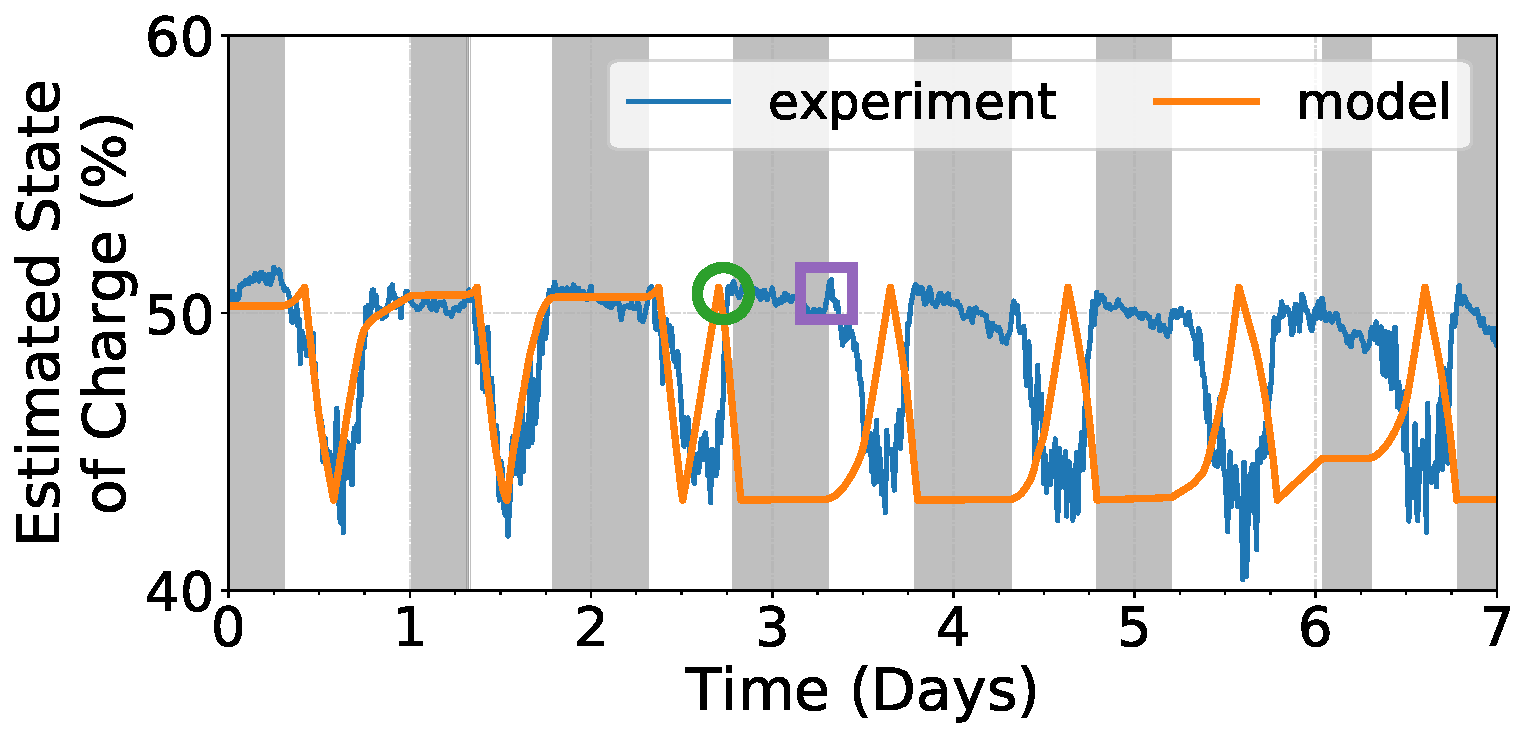
\includegraphics[width=\linewidth]{figs/capacity/experiment_soc/exp_vs_sim_soc}
    \caption{Permamote}
    \label{fig:eval:soc}
  \end{subfigure}
    \caption{Model comparison to deployed hardware.
    \normalfont
    Data from a three month deployment of two systems is used to verify our model.
    (a) We use three weeks of lux measurements %from a month-long deployment
    to estimate irradiance and model the number of packets transmitted by an
    intermittent node. Average daily error is 15\%, with a standard deviation
    of 17\%. (b) We model and measure a \name's state of charge while running a
    ``sense and send'' workload with a 1\,s period for a week, beginning at
    midnight on the first day. Secondary charging hysteresis
    limits of the devices are set at 51\% and 43\%. Shaded regions
    represent periods of low harvestable potential
    (<\,15\,\textmu W/cm\textsuperscript{2}),
    i.e. nighttime. For the first two days, model predictions
    closely track the experimental measurements. Errors
    in hysteresis and irradiance estimation cause the model to reach its upper
    hysteresis sooner than the experiment does, annotated by the
    \textbf{\textcolor{fig-green}{green circle}}. In actuality, the device
    exits charging hysteresis at the peak marked with the
    \textbf{\textcolor{fig-purple}{purple square}}.
    More importantly, the
    frequency and length of periods spent using harvested
    energy collected in the secondary-cell (downward slopes) are identical.
    %For the intermittent node we see our model
    %underestimate the number of transmitted packets by 10-20\% except for the
    %first day which predicts significantly more packets.  We believe this error
    %is primarily due to a piecewise linear estimation of irradiance from our
    %collected illuminance data, when in reality the relationship is complex and
    %non-linear.  For (b) we estimate the state of charge of \name
    %based on the secondary
    %cell voltage. Differences between the estimated state of charge and the
    %modeled state of charge are primarily due to inflated voltage during
    %charging and voltage droop and bounce back when \name
    %draws current from the secondary-cell.
    %Even though estimated state of
    %charge is not accurate due to this voltage swing, it is clear that the
    %timing of charge and discharge aligns between the model and the
    %experimental data.
    }
\end{definefigure}

\begin{definefigure}{fig:evalcmp}
    \centering
    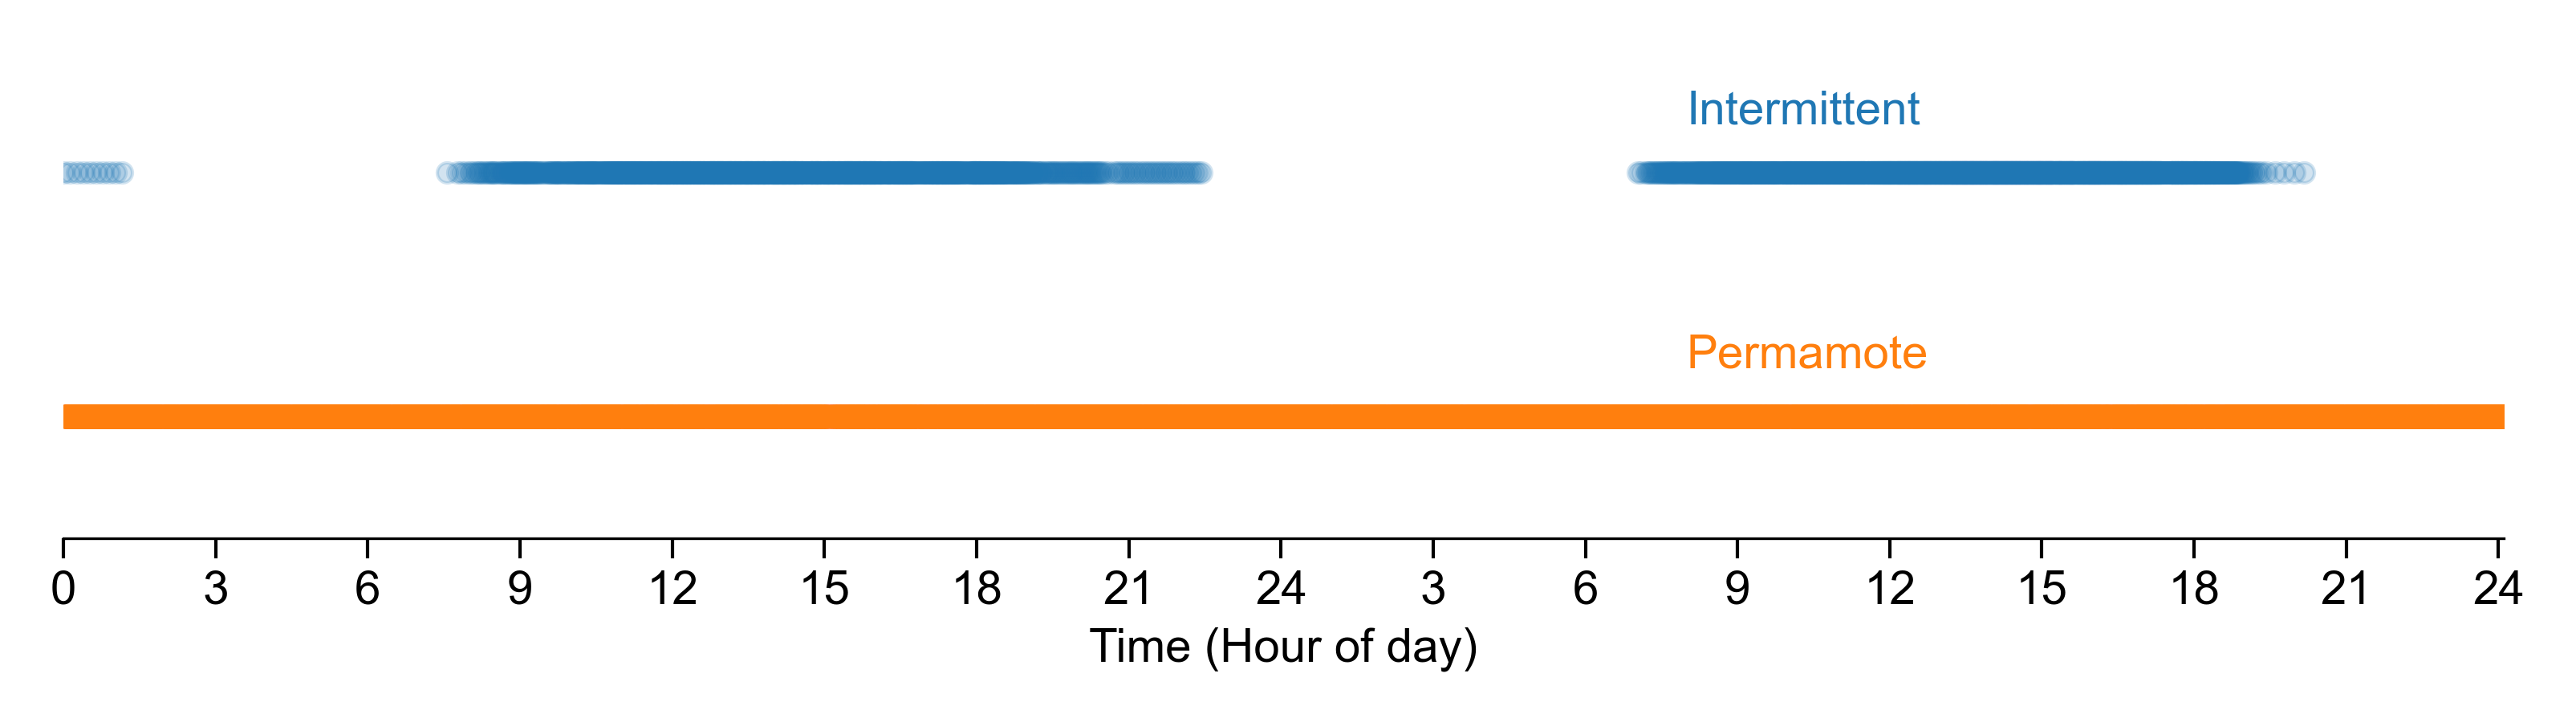
\includegraphics[width=\linewidth]{figs/capacity/experiment_sys_compare/exp_packets_recv}
    \caption{
      \normalfont
        Packets received over two days.
      This figure compares the reliability of an
      intermittent design and \name. \name sends a packet every second and does
      so without fail, while the intermittent system is only able to send when
      light is available.
      %This results in periods at night where the
      %intermittent device does not harvest enough energy to sustain operation.
      }
\end{definefigure}
\placefigure{tab:related}


\section{Summary}

\chapter{A Quantitative Evaluation of Energy Storage}
\label{chap:battery}

From the previous chapter, I have identified the value of properly sizing energy capacity in an energy harvesting design to increase energy capture and system reliability. 
Many modern energy harvesting sensor designs have utilized capacitors in their designs, which severely limit energy capacity.
Many modern platforms are attempting to push the energy bounds of sensing, computation and networking, and have begun incorporating supercapacitors to provide the necessary energy to make certain applications feasible~\cite{nardello2019camaroptera}.
These decisions are made despite the obvious option for energy capacity: batteries.
%Due to an increased need for energy storage to enable more advanced sensing and processing, the majority of modern batteryless research energy harvesting platforms utilize supercapacitors instead of tantalum or ceramic capacitors due to their superior energy density.
These designers have eschewed batteries as an option, despite their vastly superior energy density, dismissing them qualitatively as 
bulky~\cite{hesterNew17, hesterTragedy15, hesterFlicker17, hesterTimely17, yervaGrafting12},
inefficient~\cite{hesterNew17, hesterTragedy15, hesterFlicker17, hesterTimely17},
expensive~\cite{hesterNew17, hesterTragedy15, hesterFlicker17, hesterTimely17},
short-lived~\cite{hesterNew17, hesterTragedy15, hesterFlicker17, hesterTimely17, colinReconfigurable18, luciaIntermittent17, yervaGrafting12}.
%high-maintenance~\cite{hesterNew17, hesterTragedy15, hesterFlicker17, hesterTimely17, colinReconfigurable18, luciaIntermittent17},
temperature-sensitive~\cite{hesterNew17, hesterTragedy15, hesterFlicker17, hesterTimely17, colinReconfigurable18, luciaIntermittent17},
%difficult to monitor~\cite{hesterNew17, hesterTragedy15, hesterFlicker17, hesterTimely17, colinReconfigurable18, luciaIntermittent17},
%fragile~\cite{hesterNew17, hesterTragedy15, hesterFlicker17, hesterTimely17},
and dangerous~\cite{hesterNew17, hesterTragedy15, hesterFlicker17, hesterTimely17}. 
%These qualitative claims against batteries were valid when considering some of the first available rechargeable batteries. 

In this chapter, I reexamine each of these arguments with respect to modern capacitor, supercapacitor, and battery technology. 
While the early battery design of one or two decades ago were certainly guilty of many of the complaints against them, new 
battery electrode materials and improved lithium-ion manufacturing processes have produced appealing options for miniature energy storage 
that do not possess the same negative qualities as older battery technology. 
%These new batteries still possess orders of magnitude more energy density than capacitors and supercapacitors.
New battery technology paired with newly available low power energy harvesting and battery management ICs~\cite{bq25505,adp5091} enables the design of high-capacity energy harvesting systems.
Despite improvements, batteries still underperform in some metrics compared to supercapacitors, but these deficiencies are likely inconsequential for the majority of wireless sensor applications, and the substantial increase in energy capacity outweighs any detracting tradeoffs.\\

\begin{landscape}
\placefigure{tab:battery:cost}
\end{landscape}

\section{Energy Storage Technology}
\label{sec:battery-new}

I summarize the notable characteristics of various examples of capacitors, supercapacitors, and batteries in \cref{tab:battery:cost}. Many of the capacitors and supercapacitors in this table were chosen based on their inclusion in some contemporary batteryless platforms, including the Solar Monjolo~\cite{campbellEnergy14}, Flicker~\cite{hesterFlicker17}, Capybara~\cite{colinReconfigurable18}, and Camaroptera~\cite{nardello2019camaroptera}.
The selected batteries represent some of the smallest lithium-based cells that are commercially available. 
This section serves to explain the characteristics of various possible energy storage technologies for low power energy harvesting applications, as a prelude to deeper dives on particular aspects and comparisons.

\subsection{Ceramic and Tantalum Capacitors}
Along with chip resistors, the multilayer ceramic capacitor (MLCC) is the most widely used passive component in modern electronics. MLCCs are essentially a parallel connection of many cearamic plate capacitors, packaged in a small form factor~\cite{pan2010brief}. Traditionally, MLCCs are used for two applications: resonant circuits and filters and power supply bypass and decoupling~\cite{pan2010brief}. With sufficient capacitance, MLCC capacitors meant for power supply decoupling can act as the sole energy storage in a system~\cite{hesterFlicker17,yervaGrafting12,campbellEnergy14}. However, the energy storage and density of MLCC components is limited, and is often only enough to support a single small operation, like operating a sensor and transmitting the results over a radio. Similarly, tantalum capacitors are often used for power supply bypass and decoupling. Tantalum capacitors consist of a tantalum metal anode and a solid electrolyte as a cathode, separated by a solid dielectric~\cite{gill1994basic}. They generally provide more capacitance per volume than MLCCs, but are polar and have worse efficiency.
Tantalum capacitors also do not exhibit any aging effects, whereas MLCCs experience slight capacitance change over long periods of time~\cite{kemetUpdate}.
Compared to batteries and supercapacitors, MLCC and tantalum capacitors provide infinitely longer lifetimes and higher power density, but are severely limited in energy capacity and density.

\subsection{Supercapacitors}
Electrochemical double layer capacitors (EDLC) are the most common type of supercapacitor, and is utilized in many batteryless platforms~\cite{colinReconfigurable18,libich2018supercapacitors,nardello2019camaroptera}.
Supercapacitors generally consist of electrodes separated by a liquid electrolyte, like batteries, however energy accumulation is through electrostatic interaction instead of chemical reactions~\cite{libich2018supercapacitors,vangari2013supercapacitors}.
EDLCs achieve significantly higher energy density than MLCC and tantalum capacitors due to their large effective surface area and very small charge separation distances. Supercapacitors are also durable and long-lived, capable of millions of cycles~\cite{libich2018supercapacitors}. 
supercapacitors excel in high power, high cycling applications, where large amounts of charge must be stored and provided quickly, at a high frequency.
However, they offer lower power densities due to higher internal resistance compared to MLCC and tantalum capacitors~\cite{vangari2013supercapacitors}. 

\subsection{Li-ion}
Lithium-ion batteries encompass all batteries that utilize lithium ions for charge transfer. These batteries are well known for their superior energy density, and are used in small wireless and portable consumer electronics as well as in large multi-cell configurations in electric vehicles.
Like all batteries, Li-ion batteries consist of two oppositely charged electrodes separated by an electrolyte. The electrodes consist of a negatively charged anode and positively charged cathode. During discharge, Li\textsuperscript{-} ions move from the anode through the electrolyte to the cathode, and during charge they move from the cathode to the anode.
Lithium polymer (Lipo) batteries, most commonly used in consumer electronics, utilize a dry or gel electrolyte, while coin cells or cylindrical Li-ion cells utilize a liquid electrolyte. 

There are many different types of li-ion batteries, utilizing different anode, cathode, and electrolyte materials. Most modern Li-ion cells primarily utilize graphite as an anode material, and lithium nickel manganese cobalt oxide
(LiNi\textsubscript{0.33}Mn\textsubscript{0.33}Co\textsubscript{0.33}O\textsubscript{2} or NMC for short) as a cathode material~\cite{nitta2015li}.
These cells offer a nominal voltage of 3.7\si{\volt}, high energy density, and long lifetimes. 
The choice of NMC provides several benefits over earlier designs that utilize 
LiCoO\textsubscript{2} (LCO) or LiMn\textsubscript{2}O\textsubscript{4} (LMO) for cathode materials.
LCO lithium batteries are notorious for their thermal instability and fast capacity fade at high current rates or deep cycling~\cite{nitta2015li}. 
Cobalt is also a toxic and expensive metal to produce. 
LMO lithium batteries are cheaper, have higher power density, and have significantly better thermal stability than LCO cells, but have lower energy density and still have poor cycling stability, especially at higher temperatures~\cite{nitta2015li}.
The combination of nickel, manganese, and cobalt in NMC cathodes results in higher structural stability, longer lifetimes, and less reliance on expensive transition metals~\cite{nitta2015li}. 

Batteries that utilize LCO cathodes have the propensity to ignite or explode due to thermal runaway when stressed thermally, mechanically, or electrically~\cite{doughty2012general}. This is primarily due to the cathodes releasing oxygen at high temperatures, which start an exothermic reaction with the organic parts of the cell~\cite{doughty2012general, nitta2015li}. Like LCO, the newer NMC cathode material is still susceptible to thermal runaway with abuse, however the peak magnitude of self-heating on runaway is an order of magnitude less than that of LCO, and onset is delayed and begins at a higher temperature~\cite{doughty2012general}.
Batteries with LMO cathodes are safer than both LCO and NMC, but have poor cycle cycling lifetime which has limited the technology's commercialization. 

\subsection{Lithium Iron Phosphate}
Lithium iron phosphate  (LiFePO\textsubscript{4}, or LFP), is a more recently commercialized cathode material and stands to offer similar safety and power capability to LMO while offering long lifetimes similar to NMC~\cite{preger2020degradation, nitta2015li}.
Batteries that utilize LFP as a cathode material possess a lower nominal voltage (3.2\si{\volt}), and lower energy density than LCO and NMC batteries. However, LFP 
cathodes offer higher cycle stability and lifetime, have lower thermal sensitivity, and are cheaper to produce than cobalt and manganese-based cathodes~\cite{doughty2012general,nitta2015li,preger2020degradation}. LFP cells are also very safe compared to NMC and LCO cells. The only thermal runaway experienced by LFP batteries is dominated by reactions between the electrolyte and graphite anode, which decomposes at high temperatures~\cite{doughty2012general}. 

\subsection{Lithium Titanate Oxide}
Perhaps the most promising replacement for graphite anodes is lithium titanate oxide (Li\textsubscript{4}Ti\textsubscript{5}O\textsubscript{4}).
Lithium titanate oxide, abbreviated LTO, is usually paired with an LMO cathode, and sometimes an NMC cathode~\cite{nitta2015li, belharouakElectrochemistry11, sandhya2014lithium}. LTO offers superior thermal stability, high discharge/charge rates, and longer lifetimes compared to graphite. These improvements come at a cost of the more expensive titanium compound, and a lower energy density and nominal voltage (2.4\si{\volt})~\cite{nitta2015li,sandhya2014lithium}. Cells that incorporate LTO anodes are also extremely safe compared to those that use graphite~\cite{nitta2015li, belharouakElectrochemistry11, sandhya2014lithium}. Unlike graphite, LTO anodes do not produce Li dendrites after considerable cycling~\cite{nitta2015li}. This reduces the risk of inadvertent internal shorts and thermal runaway. LTO anodes also remain stable and do not break down at high temperatures~\cite{belharouakElectrochemistry11}.

\subsection{Solid-state}
All cylindrical or pouch Li-ion batteries employ a liquid or gel electrolyte of lithium salts dissolved in an organic, non-aqueous solvent~\cite{doughty2012general}. Liquid electrolyte requires specific packaging to prevent leaks, and an internal separator to prevent shorts between the electrodes. This limits the miniaturization of Li-ion batteries, as this packaging is increasingly difficult to manufacture at smaller sizes. This results in smaller batteries that have uncharacteristically high internal resistance and lower energy density compared to larger cells with the same chemistry.
The organic solvent used in liquid and gel electrolytes also can react exothermically with any oxygen released upon the breakdown of electrode material and cause thermal runaway. In addition to developing new anode and cathode materials to mitigate this, researchers and companies have also begun experimenting with replacing the non-solid electrolyte non-reactive alternatives. Solid-state batteries are safer, due to the use of non-reactive solid electrolytes, come in smaller packages, offer longer lifetimes, and have very low self-discharge~\cite{kim2015review}. However, solid-state batteries generally have limited energy and power density and high internal resistance compared to aqueous Li-ion cells. Solid-state batteries are also currently expensive to manufacture, and their commercial viability has been limited~\cite{kim2015review}.

\subsection{Summary}
Capacitors possess superior power density and have functionally infinite lifetimes, but can only store minute amounts of energy. Supercapacitors provide one to two orders of magnitude more energy density than MLCC and tantalum capacitors, at the cost of reduced power density, and more limited lifetimes. By contrast, batteries offer one to two orders of magnitude more energy density than supercapacitors. However, batteries do have limited lifetimes based on cycles, are more temperature sensitive, and some can be dangerous if mishandled. 

In the rest of this chapter, I seek to explore these comparisons in more depth. The following sections directly analyze each of the high-level qualitative arguments that "batteryless" platform designers have leveled against batteries. Namely, that they are bulky, inefficient, expensive, short-lived, temperature-sensitive, and dangerous. 


\section{Volume and Density}
\label{sec:battery:density}
Arguments that deride batteries as bulky are likely directly comparing the size of a small battery to that of single tantalum or ceramic capacitor, without considering energy and power density. Modern, commercially available miniature batteries are comparable in volume to many supercapacitors, and even a banked combination of ceramic and tantalum capacitors, while offering substantially more energy density and an acceptable power density. In this section, I explore the "bulkiness" of capacitors, supercapacitors, and batteries in the context of energy and power density. Here, I am considering volumetric density (\si[per-mode=symbol]{\Wh\per\liter}  and  \si[per-mode=symbol]{\watt\per\liter}) instead of specific energy and power (\si[per-mode=symbol]{\Wh\per\kilo\gram} and  \si[per-mode=symbol]{\watt\per\kilo\gram}, respectively) to better compare the volume of these energy storage options. The energy density and power density of various capacitors, supercapacitors, and batteries are directly compared in \cref{fig:battery:ragone}.

\placefigure{fig:battery:ragone}

\subsection{Energy Density}
Energy density should be the primary consideration for energy harvesting power supply design to maximize energy capacity while simultaneously minimizing volume. 
The energy stored in a capacitor is calculated in one of two ways:

$$E_{eff_{cap}} = \frac{1}{2} C (V^2 - V_{min}^2)$$
$$E_{total_{cap}} = \frac{1}{2} C V^2$$

\noindent Where $E_{eff}$ and $E_{total}$ is the effective and total energy stored in a capacitor, respectively. These amounts are defined by the capacitor's capacitance $C$, and the applied voltage $V$, and the minimum voltage $V_{min}$. Usually $V_{min}$ represents the minimum to do something useful. Often this is the minimum open circuit voltage to cold start a boost regulator, between 400\si{\milli\volt} to 600\si{\milli\volt}~\cite{adp5091,bq25505,max17222}. 
For simplicity, I use $E_{total}$ to determine energy capacity and density. For most capacitors, the unusable energy represented by $E_{eff_{cap}}$ is negligible compared to the total energy. Likewise, energy stored in a battery is estimated as follows:

$$E_{bat} \approx Q V_{nom}$$

\noindent Where $Q$ is the charge capacity (often denoted in terms of \si{\Ah}) and $V_{nom}$ is the battery's nominal voltage. Nominal voltage represents an average of the battery's voltage curve over the course of a charge/discharge cycle. The nominal voltage and capacity of a battery are provided by the manufacturer and are almost always included in a datasheet.

A selection of capacitor, supercapacitor, and battery energy capacities and densities are summarized in \cref{tab:battery:cost}, and their energy density is compared in \cref{fig:battery:ragone}. Among this selection, small batteries are 50-1000x more energy dense than supercapacitors and three to five orders of magnitude more dense than ceramic and tantalum capacitors. Li-ion and LiPo batteries are the most energy dense among all options. Solid-state batteries are an order of magnitude less energy dense than those with aqueous electrolytes, but still an order of magnitude more dense than supercapacitors. 

Several of these capacitors, supercapacitors and batteries are shown visually in \cref{fig:battery:sizes}.
The capacitor and supercapacitor configurations are based on examples from batteryless platform designs described in the literature~\cite{hesterFlicker17, campbellEnergy14,colinReconfigurable18}.
The batteries shown in \cref{fig:battery:sizes} are
as small as 88\si{\milli\meter\cubed}, and resemble small through-hole
capacitors and coin cells. Battery \textbf{(b)} is smaller in volume than many of the capacitor
configurations presented in the literature, only outdone by systems like Flicker \textbf{(a)} which utilize only a few ceramic capacitors~\cite{hesterFlicker17}.
This small LTO battery offers 3.7x 
more energy storage and 50x more energy density than the largest supercapacitor presented (\textbf{h}). When considering the size of other components in the system, most notably the harvester (solar panel, thermocouple, or piezoelectric device), the combination of ICs, and large sensors like a PIR motion sensor, the size of small rechargeable batteries is inconsequential. 
To my knowledge, the Michigan Micro Mote is the smallest energy harvesting system, occupying a volume on the order of a single ceramic capacitor~\cite{lee13modular}. Despite its small size, it utilizes a thin film solid-state lithium battery for energy storage due to its superior energy density over any capacitor or supercapacitor option.
When one considers energy density instead of purely volume, capacitors and supercapacitors are significantly more bulky than batteries.

\placefigure{fig:battery:sizes}

\subsection{Power Density}
In addition to energy density, power density is also an important metric to consider for a design. 
Common wireless sensor workloads are characterized by very low sleep currents punctuated by infrequent pulses of high current, usually a radio transmission. Energy storage must provide sufficient peak power to drive these short pulses, but largely, these applications require low continuous power. The maximum peak power is largely dependent on equivalent series resistance (ESR) of the storage device, represented by an internal series resistance to the capacitor or battery cell. 
Internal resistance for both supercapacitors and batteries is temperature and age dependent. Both storage elements experience increased ESR at temperature extremes, and experience increased ESR as they age.
The internal resistance of capacitors and supercapacitors is also frequency dependent, and usually reported for 1\si{\kilo\hertz}. This value is generally related inversely with frequency for frequencies below the capacitor's self-resonance~\cite{murataESRArticle}. For the relatively low frequency of charge/discharge cycles characteristic of energy harvesting devices, actual ESR is likely higher than reported for supercapacitors.

Internal capacitor, supercapacitor, and battery resistance incurs a voltage drop over this resistance which is especially noticeable and detrimental during high  current loads.
Ceramic and tantalum capacitors have negligible ESR and incomparably high power density, so I focus on comparing the power density of supercapacitors and batteries.
There are two different metrics for quantifying power output of supercapacitors and batteries. The first is effective power $P_{eff}$, and represents the maximum sustainable continuous power that can be provided. The second is peak power $P_{max}$ and represents the maximum possible current that can be provided in short pulses. These metrics are defined differently for supercapacitors and batteries. For a supercapacitor, power output is defined as follows~\cite{IEC62391}:

$$P_{eff_{sc}} = \frac{1}{8} \frac{V^2}{R_i}$$
$$P_{max_{sc}} = \frac{1}{4} \frac{V^2}{R_i}$$

\noindent Where $V$ is the voltage applied to the capacitor, and $R_i$ is the internal resistance, or ESR. For batteries, these metrics are defined as follows:

$$P_{eff_{bat}} = I_{cont} V_{nom}$$
$$P_{max_{bat}} = I_{max} V_{nom}$$

\noindent Where $I_{cont}$ and $I_{max}$ are the battery's rated continuous and peak pulsed current respectively. These metrics are provided by the battery manufacturer and often included in the battery datasheet. The continuous and peak currents are often defined in terms of the C-rate, or a proportion of the rated capacity (in units of \si{\Ah}). For example, the 1C rate of a 100\si{\milli\Ah} battery is 100\si{\milli\ampere}, and the 2C rate is 200\si{\milli\ampere}. 
Continuously charging and discharging a battery beyond its normal rate will result in cycles that deliver less energy than rated, and eventually damage to the cell resulting in capacity fading. 
For sake of comparison, I use $P_{eff}$ in \cref{tab:battery:cost} for batteries and supercapacitors, as it is a more conservative measure of the energy storage power capability. 

Among the supercapacitors and batteries featured in \cref{tab:battery:cost}, supercapacitors provide 10-400x higher power density over batteries. 
However, one supercapacitor outlier provides the least power density of all options. Like energy density, power density is also directly compared in \cref{fig:battery:ragone}.
Despite their superior power density, most applications do not require the higher power density afforded by supercapacitors. 
It is hard to imagine a \textit{low power} energy harvesting application that must source more than a few to a few hundred \si{\milli\ampere} at 3\si{\volt} infrequently, never mind continuously. 
Solid-state batteries are more power limited than other battery types. Despite their low energy capacity they are able to supply high C-rates, between 15-50C. This corresponds to currents on the order of 10\si{\milli\ampere}.
Conventional Li-ion and LiPo cells can generally source 1C continuously. The smallest Li-ion cell listed in \cref{tab:battery:cost} can provide 11\si{\milli\ampere} continuously, and the largest can provide 80\si{\milli\ampere}. The LiPo cell presented can supply 40\si{\milli\ampere} continuously. 
Small LTO and LFP cells are capable of very high C-rates, often between 20-40C for LTOs, and 10-20C for LFP~\cite{lifepo4Datasheet,LTODatasheet,LTODatasheet2}.
The smaller LTO battery listed in \cref{tab:battery:cost} is able to source 18\si{\milli\ampere}, while the larger LTO and LFP cells can source between 400-700\si{\milli\ampere} continuously. 
This power capability is more than sufficient for the majority of applications, either indoors with PANs, or outdoors, with cellular or LPWANs~\cite{nrf52840,ghena2019challenge}.

Another consideration for power capability and ESR is the effect of voltage drops during high power loads. If a voltage drop is sufficiently large, it can drop the supply to a level unusable by a voltage regulator or CMOS logic. This could effectively render part of the power storage unusable in an unpredictable manner. This effect is particularly detrimental for supercapacitors. While ESR is comparable between batteries and supercapacitors, the stability of provided voltage is not. Batteries provide a stable voltage curve centered around their nominal voltage, and voltage drops due to ESR can still result in a usable voltage even when almost empty. Supercapacitors, on the other hand, experience a (approximately) linear decrease in voltage with current until empty. This means that, depending on the load (in intensity and frequency), a large load and subsequent voltage drop could occur that causes a system brown-out, potentially corrupting state, or an unexpected reset. 


\section{Efficiency}
\label{sec:supercapvbattery}
At a high level, the efficiency of an energy storage element can be defined as the actual proportion of stored energy that is used to perform a desired task or application. Batteries have been derided as "inefficient" by batteryless platform designers, however
both supercapacitor and battery technology exhibit the same two phenomena that causes inefficiency, and generally to the same extent. 
The first phenomena is power dissipation over the internal resistance of the device. The second is self-discharge or leakage, which is represented by an internal parallel resistance to the capacitor or battery.
This section seeks to quantitatively compare these two sources of inefficiency for supercapacitors and batteries.

\subsection{Internal Resistance}
The power dissipated over the internal resistance, or ESR, of an energy storage element can be calculated as follows:

$$P_{i} = R_{i} I^2$$

\noindent Due to the squared relationship of power to current, high current loads, such as a radio transmission or long computation, are the primary cause of ESR power losses. The total power required to drive a load, including losses over internal resistance, can be defined as:

$$P_{total} = P_{l} + P_{i}$$
$$P_{total} =  I V + R_{i} I^2$$

\noindent Where $P_l$, $I$ and $V$ are the power, current, and voltage required to drive an intended load. Power inefficiency due to ESR can be very costly when considering high current loads.

With a subset of the capacitors and batteries mentioned in \cref{tab:battery:cost}, an 8\si{\milli\ampere} BLE
transmission from a steady 3\,V would incur less
than 0.03\% in resistive loss from a tantalum capacitor, a 2.1\% loss from the 1.8\si{\milli\Ah} LTO battery, and 6.3\% loss from the 7.5\si{\milli\farad} supercapacitor. A 130\si{\milli\ampere} LoRa transmission would incur a 0.43\%, 25\%, and 52\% overhead, respectively~\cite{ghena2019challenge}. These selections represent some of the worst performing examples in terms of ESR. 
For most supercapacitor and battery product lines, as they get smaller, capacitance and capacity decreases while ESR increases. When the surface area between cell electrodes decreases, this limits the flux of ions traveling between electrodes. This is manifested as an increased internal resistance.
This has traditionally been an issue for small Li-ion batteries. However, the recent commercialization of new manufacturing processes and new cathode and anode materials that increase electrode surface area has led to small form factors with lower ESR, on the order of 1-2\si{\ohm}~\cite{millibatNimbus}. Current solid-state battery technology still struggles with ESR, with values at or above 100\si{\ohm}~\cite{stEnfilm,tdkCeraCharge}.
In \cref{tab:battery:cost}, there are several batteries and supercapacitors that exhibit much lower ESR, on the order of 1\si{\ohm} or less, and are thus more efficient with high current loads. 
The 20\si{\milli\Ah} LTO battery is in the same product line as the 1.8\si{\milli\Ah} cell, but has 15x less ESR. This cell would only incur a 0.15\% and 2.3\% loss on the respective BLE and LoRa transmissions.
%For high current loads, it is very important to not only pick a storage element that can support the load, but one that also has a low internal resistance to energy wasted over the internal resistance. 
Generally, there are options for both supercapacitors and batteries that offer comparable ESR efficiency. %In this respect, batteries \textit{are not} inefficient.


\subsection{Self-Discharge}
In addition to an internal series resistance, capacitors and batteries both feature a non-ideal parallel resistance that causes a continuous self-discharge.
The self-discharge of supercapacitors and batteries is generally dependent on their size and temperature. Larger capacity/capacitance batteries and capacitors from the same product line will exhibit more self discharge than smaller ones. 

The batteries selected in \cref{tab:battery:cost} typically exhibit less than 500\si{\nano\ampere} self-discharge in standard environmental conditions. Solid-state batteries exhibit even less self discharge, at similar rates to capacitors. Notably, many types of Li-ion and LiPo batteries also require additional protection circuitry to prevent deep discharges and overcurrent charging/discharging. This additional circuitry incurs additional self-discharge. However, extremely efficient options exist to manage small batteries~\cite{ltc4071Datasheet,bq25505,adp5091}. The LTC4017 requires only 550\si{\nano\ampere} when in operation, and features a very low disconnect current (<1\si{\nano\ampere}) to extend shelf-life~\cite{ltc4071Datasheet}.
This amount of self-discharge is negligible when considering the average sleep currents of common sensors and MCU options. Generally, sleep currents will still be dominated by memory retention and low frequency clock operation, on the order of a few \si{\micro\ampere}. 

While the self discharge of capacitors and supercapacitors appears lower than batteries, this is partially due to how it is measured and rated. However, the self discharge of supercapacitors is actually is comparable to that of batteries when considering short term post-charge behavior.
Supercapacitors exhibit a pronounced, non-ideal phenomena known as dielectric absorption~\cite{kundert2008modeling}. Dielectric absorption represents a decreasing exponential decay of the supercapacitor voltage immediately after charging. After hours or days, self-discharge is dominated by a linear leakage current. The magnitude of the decay depends on the initial voltage, temperature, and duration of the charge~\cite{kowal2011detailed}. Datasheets generally specify supercapacitor leakage after a subsequent 24 hour constant voltage charge and 1 hour open circuit period. This is sufficient time for the contribution of dielectric absorption to be rendered negligible. After this time, only the internal parallel leakage resistance is a factor.

In the short term, however, the discharge due to dialectric absorption dominates. For example, after an hour of constant voltage charging, the 33\si{\milli\farad} BestCap supercapacitor listed in \cref{tab:battery:cost} experiences an average of 300\si{\nano\ampere} self-discharge over a 3 hour window. Considering the common use case of supercapacitors in batteryless systems, where any captured energy is immediately used whenever it is available. This short term cycle use case means that energy is never stored for an extended period of time, and dialectric absorption is a primary factor in self-discharge for batteryless systems. While I have not characterized the self-discharge of each individual supercapacitor listed in \cref{tab:battery:cost}, this phenomena is inherent to electrochemical capacitor technology.

%In addition to additional leakage due to absorption effects, some batteryless sensor designs employ a bank of multiple parallel capacitors and supercapacitors to build up enough energy storage to support their workload~\cite{colinReconfigurable18}. Since these capacitors are in parallel, their internal resistances are summed. 

Generally, one can expect the short-term self-discharge of supercapacitors to be comparable with batteries. In either case, self-discharge is not sufficient to warrant discounting either option for a low power design. When considering the impact of self-discharge with that of ESR loss, there are suitable options from both technologies that would provide satisfactory performance.

\placefigure{fig:battery:eperd}

\section{Expense}
\label{sec:battery:cost}
Like the bulkiness argument, the claim that batteries are "expensive" is only valid when directly comparing the cost of a battery to that of single ceramic or tantalum capacitor. This view is reductionist, and this section seeks to explore this argument in more detail.

Most batteries are actually comparatively cheap when considering energy capacity and density. Solid-state batteries are still costly, as they are a newly commercialized technology and their manufacture is still expensive. 
A single battery provides significantly more energy storage per dollar than any capacitor, supercapacitor, or banked configuration.
\Cref{fig:battery:eperd} illustrates this by comparing the energy per dollar one can expect from capacitors, supercapacitors, and batteries. 
Solid-state batteries offer a similar magnitude of energy per dollar to supercapacitors.
Other battery types offer several orders of magnitude more energy capacity per dollar than capacitors and supercapacitors.

The expensiveness of capacitors is accentuated when considering that some designs require multiple parallel capacitors or supecapacitors to build up enough energy capacity. For example, the Capybara design is configured with 14 of the 7.5\si{\milli\farad} Seiko supercapacitors, each costing ~\$2.42 USD, for a total of \$33.88~\cite{colinReconfigurable18}. The small 1.8 \si{\milli\Ah} battery still offers 4.4x the energy capacity of these 14 parallel supercapacitors, for only \$1.25.
It would require 61 of the Seiko supercapacitors to provide the same amount of energy capacity as the 1.8\si{\milli\Ah} battery. Those 61 supercapacitors would cost \$148.

Besides the Seiko supercapacitor, several of the selected supercapacitors in \cref{tab:battery:cost} are as expensive or more expensive than the selected batteries~\cite{murataCap,kemetCap,seikoCap,bestCap}.
Small, 2-50~mAh LTO batteries can be purchased for
\$6.75 USD each from US distributors and \$1.25 USD each from Chinese manufacturers, even in small quantities~\cite{LTODatasheet, LTODatasheet2}. 

%and the
%cost of other key components in an energy harvesting system, like the
Also, when considering the cost of other components in a wireless energy harvesting system, like
an SoC~\cite{nrf52840}, harvester~\cite{sanyoSolarCell} and sensors~\cite{si7021},
which each cost around \$5 USD each in low quantities, a battery will not constitute
the driving cost. Batteries are by far the most cost effective option for providing energy capacity. The argument that they are too expensive for a sensor design says nothing to the comparable cost of supercapacitors, and entirely ignores the benefits of the superior energy density of batteries. 


\section{Lifetime}
Batteries are often considered "short-lived" due to their limited cycle lifetimes, especially when compared to ceramic and tantalum capacitors. 
Ceramic and tantalum capacitors lifetimes are estimated to be thousands to millions of years with proper voltage derating and when used at room temperature~\cite{kemetLife}. 
The lifetime of capacitors, supercapacitors, and batteries generally refers to the lifetime before the device experiences parametric failure. Parametric failure is when the device is no longer within spec, usually when rated capacitance/capacity is lower than 20\% its original value, or when ESR or other parasitics are sufficiently higher than rated.
This section serves as an effort to quantify and compare battery lifetime with capacitors and supercapacitors, and to investigate methods for elongating their cycle lifetimes.
While modern battery technology will never compete with the longevity of capacitors, for low power energy harvesting, cycle lifetime is unlikely to be the limiting factor on the lifetime of a battery, never mind the system as a whole. 

%Perhaps the primary reason for the excitement around batteryless platform is the claim of infinite lifetimes of their power supplies. And this claim has merit when considering ceramic and tantalum capacitors, 
While ceramic and tantalum capacitors can potentially last a million years, these lifetime estimates do not hold for supercapacitors, which are often rated in thousands of hours at a specified voltage and temperature (often 65-85\si{\celsius})~\cite{bestCap,murataCap}. This lifetime is further influenced by the cycling characteristic and intensity of the workload~\cite{kreczanik2013study}. For low power wireless sensors in room temperatures, with the sporadic cycling rate of an intermittent system, one can still expect lifetimes of a hundred thousand to one million hours~\cite{kreczanik2013study}. While this is a long lifetime, it is by no means infinite.

Conversely, the cycle lifetime of a battery is generally the number of full cycles at a rated continuous discharge/charge current (usually 0.5C or 1C) before the battery's capacity diminishes to 80\% of its original rated capacity.
Generally, NMC lithium batteries offer a cycle lifetime between 3000 and 5000 cycles~\cite{richter2017measurements,preger2020degradation}, compared to 300-700 cycles for LCO and LMO batteries.
For small form factor batteries, this cycle lifetime is less, and for those in \cref{tab:battery:cost}, they offer only 300-500 cycles~\cite{lipoDatasheet, millibatNimbus} at a 0.5~C charge/discharge rate.
However, new battery chemestries like LTO and LFP batteries offer between 2000 and 7000 cycles at 0.5~C~\cite{hallExperimental18, LTODatasheet, LTODatasheet2,omarLithium14, sarasketaCycle15, wangCycle11,lifepo4Datasheet, preger2020degradation}. Solid-state batteries also offer long cycle lifetimes, between 1000 and 4000 cycles for commercially available cells~\cite{stEnfilm,tdkCeraCharge}.

These rated cycle lifetimes represent the cycle life at 100\% depth-of-discharge (DoD), however battery cycle lifetime is heavily influenced by the rate of discharge, as well as the depth of discharge.
The reduction of battery DoD to 10\%
exponentially reduces cycle capacity loss, resulting in potential
lifetimes of greater than 10,000 cycles before reaching 20\% capacity degradation with LFP cells~\cite{omarLithium14, wangCycle11}. Similarly, LTO cells are estimated to sustain approximately 15,000 cycles before reaching 20\% capacity degradation~\cite{stroe2018accelerated}.
These cycle estimations for LTO cells hold true even for relatively high temperatures (50-60\textdegree
C)~\cite{wangCycle11, stroe2018accelerated}.
LTO chemistries can be expected to survive one thousand
cycles at 100\% DoD at 55\textdegree C~\cite{han2014cycle}.
Life cycle
expectations for both 100\% and 10\% DoD are summarized in
\cref{tab:battery:cost}.

On its face, several thousand cycles does not seem like a lot compared to the lifetime estimates of capacitors and supercapacitors. However, for batteries, this cycle lifetime amounts to a significant amount energy. This energy also represents a significant amount of time when considering the energy capacity of batteries, and the expected charge/discharge behavior of energy harvesting wireless sensors.
The comparatively vast energy capacity of batteries means that each cycle represents a significant amount of energy. This amount of energy can drive a low power workload for an extended period of time. For example, the representative periodic workload described in \cref{tab:capacity:rep} requires an average power of 58.6\si{\micro\watt}. For the smallest 1.8\si{\milli\Ah} battery, a single discharge cycle represents just over 3 days of continuous operation. The rated 7000 cycle lifetime of this cell represents 117 years, assuming an identical charge/discharge cycle. 

For wireless sensor workloads, battery cycle lifetime is not going to constitute the main source of failure in designs that incorporate them. Instead, limited shelf-life and poor battery management are likely to be the driving forces behind usable battery lifetimes. 
Shelf-life represents the amount of time a battery can sit uncharged before depleting itself and experiencing capacity degradation. Batteries must also be properly charged and discharged within rated current limits, and should not be overvolted or undervolted. 
It is conceivable that energy harvesting systems may be deployed in areas with little available harvestable energy, and be unable to charge their batteries for long periods of time. 
The shelf-life for lithium-based batteries is approximately one decade, however, LTO chemistries have been shown to exhibit no long-term cell
damage when undervolted, even to zero volts~\cite{brunell2016effect}.
This is a significant improvement more traditional technologies like Li-ion and LiPo which suffer capacity degradation if undervolted due to long storage and absence of charging. 
Regardless of the type of battery, designs should utilize the myriad of small battery charger and management ICs that exist to properly manage battery state and minimize the effects of shelf-life~\cite{ltc4071Datasheet,bq25505,adp5091}.

The lifetime of an energy harvesting system is also not solely dependent on the lifetime of its power supply.
Most notably, some components exhibit significant long-term calibration drift. For example, each year a humidity sensor~\cite{si7021} expects a quarter of a percent relative humidity drift, while an oscillator~\cite{txc-oscillator} expects 3~ppm drift.
There is also the question of relevancy in the face of decades of future
progress in networking, processor efficiency, and MEMS sensors. At some point, the wireless sensor platforms built today
will be obsolete and less useful, regardless of their theoretical lifetimes. Sensors do not need to last indefinitely, they need to last long enough and provide enough
benefit to justify their original deployment. Replacement and renovation is inevitable.
Conservatively, rechargeable batteries have the capability to last between 10 and 20 years when managed properly. While not cycle limited, supercapacitors have similar lifetime estimates on the order of a decade or two. 
When considering this reality, only systems that employ ceramic and tantalum capacitors can claim to support indefinite lifetimes. It is unclear that supercapacitor-based batteryless systems are any better off in terms of lifetime than battery-based systems.

\section{Temperature Sensitivity}
In addition to lifetime considerations, batteries are also notorious for their temperature sensitivity. As mentioned previously, in temperature extremes, batteries exhibit higher ESR, self discharge, and have accelerated capacity degradation. Out of the many arguments against batteries, temperature sensitivity is the most coherent. This section seeks to quantify and compare the temperature sensitivity of capacitors, supercapacitors, and batteries and identify the applications for which it has a significant impact.

Ceramic and tantalum capacitors are very temperature resistant. Of the few selected in \cref{tab:battery:cost}, both types are rated for -55 to +125\si{\celsius}~\cite{ceramicDatasheet,ceramicDatasheet2,tantalumDatasheet}. The ceramic and tantalum capacitors both exhibit approximately 10\% capacitance difference at -55 and 85\si{\celsius}. Extreme temperatures can reduce operational lifetimes, however. High temperatures can reduce expected lifetimes from 4000 years at 45\si{\celsius} to just 14 years at 85\si{\celsius} for tantalum capacitors~\cite{kemetLife}.

Supercapacitors are also rated for extreme temperatures, and those listed in \cref{tab:battery:cost} can withstand temperatures between -40 to -20\si{\celsius} on the low end to up to 70\si{\celsius}. Supercapacitors generally experience increased ESR with lower temperatures, and lifetime limits with higher temperatures~\cite{murataCap,bestCap,kreczanik2013study,murataTech}. Capacitance is generally affected by low and high temperatures. For the 33\si{\milli\farad} BestCap, at -40\si{\celsius}, ESR can increase to 20x its rated value. Similarly for the 470\si{\milli\farad} Murata capacitor, it can experience 8x its rated ESR at the same temperature. All supercapacitors have a rated lifetime in terms of hours at a specific temperature. The BestCap can withstand 1000 hours at 70\si{\celsius}, and the Murata cell is rated for 1000 hours at 85\si{\celsius} before experiencing a capacitance degradation of 20\%. For supercapacitors, the effects of extreme temperatures is actually quite severe. At cold temperatures, supercapacitors will be unable to supply current at a sufficient voltage, and at high temperatures their rated lifetime can decrease from hundreds of thousands of hours to just 1000, or from approximately 11 years to 40 days. Even a moderately high temperature of 45\si{\celsius} can reduce some supercapacitor operational lifetimes to 3 years from 14 years at room temperature~\cite{kreczanik2013study}.

Like supercapacitors, batteries experience adverse effects at extreme temperatures. At low temperatures, lithium-based batteries exhibit a reduced energy capacity, support lower charge and discharge rates, exhibit higher ESR, and can experience accelerated shelf-life and cycle aging~\cite{jaguemont2015lithium}. For a LFP battery at -20\si{\celsius}, its capacity is reduced to approximately 60\% of its original value. When this battery is stored at -20\si{\celsius} for 17 days, it experiences a further 10\% capacity degradation to 50\%, and a 16x increase in ESR to 8\si{\milli\ohm} from 0.5\si{\milli\ohm}~\cite{jaguemont2015lithium}.
If charging rates are exceeded at cold temperatures, or the battery is simply cycled at low temperatures, additional battery capacity degradation can occur. The same LFP battery as above experiences a 12\% degradation after only 12 cycles at -20\si{\celsius}~\cite{jaguemont2015lithium}.
Likewise, at higher temperatures, lithium batteries also experience accelerated aging and increased internal resistance~\cite{leng2015effect}. At extreme temperatures, some types of lithium batteries can experience thermal runaway and cause explosions or fires. These effects are rarely described and quantified in battery datasheets. Instead, manufacturers simply provide a range of operational temperatures.

Li-ion and LiPo batteries are particularly sensitive to temperature. Of those listed in \cref{tab:battery:cost}, they are generally only rated for 0-40\si{\celsius} for charging, and -20-60\si{\celsius} for discharging. I would expect them to perform worse than the metrics listed previously for the LiFeMnPO\textsubscript{4} battery.
Generally, LTO and LFP batteries perform better in extreme temperatures than traditional Li-ion and LiPo cells.
Some 
datasheets and authors report operating LTO batteries successfully as low as -30\,\textdegree C
and as high as 75\,\textdegree C~\cite{LTODatasheet2, lifepo4Datasheet, chenEvaluation15}. From their datasheet, the selected LTO cells in \cref{tab:battery:cost} exhibit a 10\% capacity degradation at -20\si{\celsius}, and a 20\% degradation at -30\si{\celsius}. At high temperatures, these cells only experience a 2\% degradation at 75\si{\celsius}, and less than 1\% at 60\si{\celsius}. LFP cells perform worse than LTO cells at lower temperatures. According to the datasheet of the cells in \cref{tab:battery:cost}, they experience 40\% capacity degradation at -20\si{\celsius}, which is in agreement with the previous section~\cite{lifepo4Datasheet, jaguemont2015lithium}. Solid-state batteries also perform relatively well in extreme temperatures due to their solid electrolyte, and there are commercial options rated for -20 to 80\si{\celsius}. However, at -20\si{\celsius}, effective capacity is reduced to just 20\% of original. For this solid-state battery, effective capacity actually increases at 80\si{\celsius} to 120\%~\cite{tdkCeraCharge}.
No information is given on temperature's effect on ESR and long-term cycle lifetime for these cells, but related work indicates these metrics would still be severely impacted by extreme temperatures.
~\cite{wangCycle11, swierczynskiInvestigation14}.

Regardless of type, lithium batteries should be kept as close to room temperature as possible, and in extreme environments like high altitudes, deserts, or even in space or close to the earth's mantle, batteries will require active heating or cooling to maintain an operational lifetime. For example, the Mars Curiosity and Perseverance rovers utilize a Radioisotope Thermoelectric Generator (RTG) to both provide heating and constant thermocouple harvesting to charge a bank of two Li-ion batteries~\cite{nasaPerseverance}. Battery packs with included (non-RTG) heaters are also commercially available for cubesat applications~\cite{nanopowerbpx}.

Batteries are not as robust as capacitors and supercapacitors when used in extreme temperatures, and will require temperature control. However, 
supercapacitors also require active temperature management to maintain long lifetimes at high temperatures. When considering common use cases for wireless sensors, the efficient and operational range of both batteries and supercapacitors encompasses all applications located in spaces that humans occupy, and likely will handle most of the range of temperatures outdoors in many locations.

\section{Safety} 
Besides temperature sensitivity, many types of lithium metal batteries are also notorious for their propensity to burn and explode under mechanical, electrical, and thermal stress.
Capacitors and supercapacitors do not exhibit same caliber of danger, and at most will "pop" if exposed to electrical stress like overcharge or a large inverted charge. 
For both batteries and supercapacitors, electrical stress is exceedingly rare for low power energy harvesting applications, especially if using a battery protection and voltage management circuit. However, in some extreme environments, mechanical and thermal stress can be an issue. 

Batteries with LCO and NMC cathodes and graphite anodes are prone to fiery explosions if mishandled. However, 
batteries that use other electrode materials, like LFP cathodes or LTO anodes, are considered much safer~\cite{doughty2012general,nitta2015li,belharouakElectrochemistry11,larssonAbuse14}.
Compared to LCO and NMC, LFP has enhanced safety and stability~\cite{larssonAbuse14}. The structure of the LFP cathode is more thermally and chemically stable.  
The LFP cathode material has been shown to not release oxygen during thermal runaway, even when fully decomposed at high temperatures. 
The P-O bond within the PO\textsubscript{4}\textsuperscript{3-} ion is stronger than that of the Co-O bond in the CoO\textsubscript{2}\textsuperscript{-}, so that when abused, oxygen is released slowly or not at all~\cite{nitta2015li}.
This results in a significantly safer cell, where any thermal runaway is dominated by anode and electrolyte reactions at extreme temperatures~\cite{doughty2012general}.

Like LFP cathodes, LTO anodes provide similar benefits over graphite anodes. Graphite is prone to expansion and contraction during charging and discharging, respectively, which causes internal damage to the cell, resulting in capacity fading and in rare cases, short circuit conditions~\cite{sandhya2014lithium}. This effect is further exacerbated at extreme temperatures. 
LTO is considered a zero-strain material, meaning it experiences very little change in its chemical structure during charging, discharging, or temperature changes, unlike graphite. When heated to high temperatures, graphite can break down and react exothermically with the electrolyte, releasing flammable hydrocarbons. By contrast, at the same high temperatures, LTO anodes do not produce heat or release any gasses~\cite{belharouakElectrochemistry11}. Beyond the anode chemical stability, the high potential of LTO anodes prevents lithium dendrites from forming upon deep cycling or after many cycles~\cite{nitta2015li}. Lithium dendrites are the main cause for internal shorts in batteries with graphite anodes. These features of LTO anodes greatly lower the risk of internal short circuits, thermal runaway, and explosions.
The solid electrolyte in solid-state batteries also substantially improves safety. A solid electrolyte is not flammable, and since it is solid, it is chemically unable to interact explosively with a decaying cathode or anode~\cite{kim2015review}.

While there is still slight potential for danger under abuse conditions for LTO, LFP, and solid-state batteries, the danger is substantially less than traditional graphite and cobalt-based lithium batteries. For LTO batteries, the danger of thermal runaway and explosion should be equivalent with that of a supercapacitor. Solid-state batteries should be even safer than supercapacitors, as EDLC supercapacitors employ an aqueous electrolyte.
The battery manufacturer for the LTO and LFP cells listed in \cref{tab:battery:cost} states in the datasheet that no battery protection circuit is necessary to ensure safety~\cite{LTODatasheet,LTODatasheet2}. 
These cells also feature a capacitor-like notched cap that fails first in the case of internal pressure and gas release.
Despite their safety, battery management is still important to limit damage to any battery and maintain capacity and performance. 
Not all lithium batteries are equivalent, and the claim that \textit{all} batteries are dangerous disregards the many safety improvements made with newer electrode and electrolyte materials.

\section{Summary}
Among the various arguments that "batteryless" platforms have levied against batteries, very few are relevant in the face of improved battery technology. Out of all addressed here, temperature sensitivity is the only real limitation of batteries. This complicates their usage in extreme environments, but by no means discounts them. Batteries can not compete against some supercapacitors in terms of power density and cycling performance, but for low power applications, this metric is inconsequential. 
In reality, batteries are by far the most energy dense rechargeable storage device developed and they provide many orders of magnitude more energy capacity per dollar than any capacitor or supercapacitor. New battery technology provides comparable efficiency, lifetime, and safety to many modern supercapacitors. 

These qualitative arguments are the same made in the early 2000s, when battery technology was admittedly not well suited for long-lived, low power applications. Two decades later, these arguments have not been revisited, and are instead used ad nauseam to further justify the design decisions made to enable indefinite wireless sensor lifetimes. 
%It has resulted in a lazy or intentionally obtuse view of energy harvesting system design research, where no thought is given to properly sizing components to optimally enable an application. 
%Instead, the decision to use a supercapacitor is the default, chosen to make an application work, but not work well. Research in this area has pivoted from trying to solve interesting and hard problems with wireless sensor networks, to creating complex and overbearing software solutions to shoehorn supercapacitors into applications they are poorly suited for. The real problem is in reality a hardware one: these platforms do not have enough energy capacity. There is also very simple hardware solution: \textbf{use a battery}. 
The choice to use a (super)capacitor has become the default, often selected to provide just enough energy storage to allow an application to function, but nowhere near enough to function well. This lack of energy capacity in the name of immortality has forced researchers to develop complex software and hardware solutions to shoehorn capacitors and supercapacitors into applications they are poorly suited for. There is a far simpler solution: \textbf{use a battery}.

\begin{definetable*}{tab:battery:cost}
    \begin{adjustbox}{width=1.3\textheight}
    \begin{threeparttable}
    \begin{tabular}{l | l | S[table-format=1.9,table-align-text-post = false] | c | S[table-format=3.3,table-align-text-post = false] | S[table-format=7.3,table-align-text-post = false] | S[table-format=3.3,table-align-text-post = false] | c | r | c | c | c | c | c}
     \multirow{2}{*}{Technology}  & {Capacitance / } &  {Energy Capacity} & {Voltage} & {Volume} & {Energy Density} & {Power Density\tnote{b}} & Temperature & ESR &  Self-Discharge &  \multicolumn{2}{c|}{Cycle Life (Cycles)\,\tnote{j}} & \multicolumn{2}{c}{Cost (USD)}\\\cline{11-14}

     & {Capacity} & {(\si{\Wh})} & {(\si{\volt})} &  {(\si{\mm\cubed})} & {(\si[per-mode=symbol]{\Wh\per\liter})} & {(\si[per-mode=symbol]{\watt\per\liter})} & (Charge/Discharge\,\textdegree C) & (\si{\ohm}) & (\si{\nano\ampere}) &  100\% DoD & 10\% DoD & US\,\tnote{m}  & China  \\
      \hline
      
\multirow{2}{*}[0.6em]{MLCC}
    & 47\si{\micro\farad}~\cite{ceramicDatasheet2}  
    & 0.000000259\,\tnote{a}
    & 6.3
    & 8.19 
    & 0.032
    & 6060000\,\tnote{c}
    & -55 - 125
    & 0.001-0.1\,\tnote{f}
    & <10\,\tnote{h}
    & $\infty$\,\tnote{k}
    & $\infty$\,\tnote{k}
    & 0.16
    & 0.03  \\
    
    & 100\si{\micro\farad}~\cite{ceramicDatasheet}
    & 0.00000139\,\tnote{a}
    & 10
    & 20.0
    & 0.069
    & 6250000\,\tnote{c}
    & -55 - 125
    & 0.001-0.1\,\tnote{f}
    & <10\,\tnote{h}
    & $\infty$\,\tnote{k}
    & $\infty$\,\tnote{k}
    & 0.31
    & 0.04  \\
                                
\multirow{2}{*}[0.6em]{Tantalum}    
    & 100\si{\micro\farad}~\cite{tantalumDatasheet}
    & 0.000000551\,\tnote{a}
    & 6.3
    & 18.6
    & 0.030 
    & 2670000\,\tnote{c}
    & -55 - 125 
    & 0.2\,\tnote{f} 
    & <10\,\tnote{h}                        
    & $\infty$\,\tnote{k}         
    & $\infty$\,\tnote{k}   
    & 0.28          
    & 0.17  \\
                                    
    & 220\si{\micro\farad}~\cite{tantalumDatasheet}
    &0.00000306\,\tnote{a}
    & 10
    & 91.0
    & 0.034
    & 1370000\,\tnote{c}
    & -55 - 125      
    & 0.07\,\tnote{f}                    
    & <10\,\tnote{h}                        
    & $\infty$\,\tnote{k}         
    & $\infty$\,\tnote{k}   
    & 0.37          
    & 0.16  \\\hline

\multirow{2}{*}[0.6em]{Supercapacitor}        
    & 7.5\si{\milli\farad}~\cite{seikoCap}   
    & 0.0000704\,\tnote{a}
    & 2.6
    & 7.2               
    & 0.980   
    & 4690
    & -30 - 70\,\tnote{d}               
    &    25\,\tnote{f}                  
    & <10\,\tnote{i}                        
    & >10000                  
    & \textemdash       
    & 2.42
    & {\textemdash}     \\
                                    
    & 33\si{\milli\farad}~\cite{bestCap}
    & 0.000139\,\tnote{a}
    & 5.5
    & 870
    & 0.159
    & 17400
    & -20 - 70\,\tnote{d}               
    & 0.25\,\tnote{f}
    & <5\,\tnote{i}
    & \textemdash             
    & \textemdash
    & 8.65
    & {\textemdash} \\
                                    
    & 100\si{\milli\farad}~\cite{kemetCap}
    & 0.000420\,\tnote{a}
    & 5.5 
    & 1130
    & 0.372
    & 33.5
    & -25 - 70\,\tnote{d}               
    & 100\,\tnote{f} 
    & <10\,\tnote{i}                        
    & \textemdash             
    & \textemdash       
    & 1.10
    & {\textemdash}     \\
                                   
    & 470\si{\milli\farad}~\cite{murataCap}  
    & 0.00115\,\tnote{a}
    & 4.2
    & 1029 
    & 1.17
    & 16500
    & -40 - 70\,\tnote{d}  
    & 0.13\,\tnote{f}
    & <1000
    & 100000+/4\,yr~\cite{murataTech}\,\tnote{l} 
    & \textemdash\,\tnote{l}   
    & 5.06 
    & 1.00  \\\hline
    
\multirow{2}{*}[0.6em]{Li-ion}        

    & 11\si{\milli\Ah}~\cite{millibatNimbus}
    & 0.0407
    & 3.7
    & 191
    & 213
    & 96.9
    & 0 - 40/-20 - 60\,\tnote{f}
    & 1\,\tnote{g}
    & \hl{XX}
    & 500
    & 10000+~\cite{guenaDepth06, millnerModeling10}
    & 4.00
    & \textemdash \\
    
    & 40\si{\milli\Ah}~\cite{40mahliion}
    & 0.148
    & 3.7
    & 1010
    & 147 
    & 44.4
    & 0 - 40/-20 - 60\,\tnote{f}
    & 3
    & 120-400~\cite{zimmermanSelf04}
    & 500
    & 10000+~\cite{guenaDepth06, millnerModeling10}
    & 1.62
    & \textemdash \\
    
    & 80\si{\milli\Ah}~\cite{millibatNimbus}
    & 0.296
    & 3.7
    & 1010
    & 295
    & 147
    & 0 - 40/-20 - 60\,\tnote{f}
    & 2\,\tnote{g}
    & \hl{XX}
    & 500
    & 10000+~\cite{guenaDepth06, millnerModeling10}
    & 7.00
    & \textemdash \\\hline
    
\multirow{2}{*}[0.6em]{LiPo}        
    & 40\si{\milli\Ah}~\cite{lipoDatasheet}
    & 0.148
    & 3.7
    & 660
    & 224
    & 224
    & 0 - 40/-20 - 60\,\tnote{f}
    & 1.5
    & 120-400~\cite{zimmermanSelf04}
    & 300
    & 10000+~\cite{guenaDepth06, millnerModeling10}
    & 4.50
    & 0.51  \\\hline
    
\multirow{2}{*}[0.6em]{LTO}

    & 1.8\si{\milli\Ah}~\cite{LTODatasheet2}
    & 0.0043
    & 2.4
    & 88.0
    & 48.9
    & 489
    & -35 - 70\,\tnote{f}
    & 8  
    & <300\,\tnote{g} 
    & 2000      
    & 10000+~\cite{hallExperimental18}
    &  {\textemdash}& 1.28  \\
    
    & 20\si{\milli\Ah}~\cite{LTODatasheet,LTODatasheet2}
    & 0.0480
    & 2.4
    & 682
    & 70.4
    & 1410 
    & -35 - 70\,\tnote{f}
    & 0.55\,\tnote{g}
    &  <300\,\tnote{g}
    & 7000
    & 10000+~\cite{hallExperimental18}
    & 6.75
    & 1.28  \\\hline
    
LFP
    & 70\si{\milli\Ah}~\cite{lifepo4Datasheet}
    & 0.224
    & 3.2
    & 1570 
    & 143
    & 1430 
    & -20 - 75\,\tnote{f}
    & 0.18
    & \hl{160}~\cite{swierczynskiInvestigation14}
    & 2000
    & 30000+~\cite{wangCycle11,sarasketaCycle15,omarLithium14}
    &  {\textemdash}
    & 1.28 \\\hline

Solid State
    & 0.7\si{\milli\Ah}~\cite{stEnfilm}
    & 0.00273
    & 3.9
    & 145
    & 18.8
    & 134.2
    & -20 - 60\,\tnote{f}
    & 100
    & <3
    & 4000
    & {\textemdash}
    & 30.00 
    & {\textemdash} \\
    
    & 0.1\si{\milli\Ah}~\cite{tdkCeraCharge}
    & 0.000150
    & 1.50
    & 14.5
    & 10.3
    & 2.07
    & -20 - 80\,\tnote{f}
    & <200
    & <80
    & 1000
    & {\textemdash}
    & 9.31
    & {\textemdash} \\
    
%\multirow{2}{*}[0.6em]{Li-Primary}  & 720\,mWh~\cite{primary2032}    & 1005\,\tnote{a}  & 716               & -30 - 60\,\tnote{f}               & {N/A\,\tnote{i}}          & 250                                   &N/A                      &  N/A              & 0.20          & 0.10  \\
%                                    & 4500\,mWh~\cite{primarycr123a} & 7830\,\tnote{a}  & 574               & -40 - 70\,\tnote{f}               & {N/A\,\tnote{i}}          & 1400                                  &N/A                      &  N/A              & 0.90          & 0.75  \\
%\multirow{2}{*}[0.6em]{Li-Thin Film}& 3.9\,mWh~\cite{thinDatasheet}  & 119              & 32.7              & -20 - 60\,\tnote{f}               & 80                        & 3.5                                   &4000                     &\textemdash        & 18.24         & {\textemdash}     \\
%                                    & 190\,\textmu Wh~\cite{thinDatasheet2} & 58        & 3.2               & -40 - 70\,\tnote{f}               & 2200                      & 0.2                                   &300                      &  5000             &  {\textemdash}& {\textemdash}     \\
   \end{tabular}
    \begin{tablenotes}[para]
        \item[a] Energy capacity calculated with rated maximum voltage.
        \item[b] Calculated with battery and capacitor effective power. \\
        \item[c] Effective power for capacitors is slightly nebulous. Here the higher end of ESR is assumed.
        \item[d] Supercapacitors experience higher ESR at lower temperatures and higher leakage at higher temperatures~\cite{murataTech}.\\
        \item[e] Lithium batteries experience higher ESR, higher leakage, lower capacity and shorter lifetimes at temperature extremes.
        \item[f] ESR is frequency dependent, supercapacitors are usually rated at 1\si{\kilo\hertz}. \\
        \item[g] Empirically tested.
        \item[h] Both tested and calculated from insulation resistance after absorption period.
        \item[i] Specification after 24\,h of charging.
        \item[j] For batteries, measured to 80\% original rated capacity.
        \item[k] Capacitor derating is not considered. With proper design principals these should be nearly infinite.
        \item[l] Supercapacitors are time rather than cycle limited. Assumes 3V, 20\,\textdegree C. No DoD dependence mentioned~\cite{murataTech}. \\
        \item[m] Prices are based on cheapest available equivalent part in quantities of 100.
    \end{tablenotes}
    \end{threeparttable}
    \end{adjustbox}
    \caption{A comparison of miniature energy storage technologies.
    \normalfont
    Data is based on specific components and their datasheets, and
    components are chosen for each category based on their inclusion in platforms described by the literature.
    Some technologies are rapidly evolving, such as supercapacitors and batteries. Other citations point to general characteristics 
    of the storage technologies not specified by their datasheets. For
    most applications, lithium-based batteries provide much higher energy density
    without reasonably impacting sensor lifetime, cost, or function.
    The minority of sensing applications, such as those operating at extreme
    temperatures, may require capacitors or active heating and cooling.}

\end{definetable*}

\begin{definefigure}{fig:battery:sizes}
  \centering
  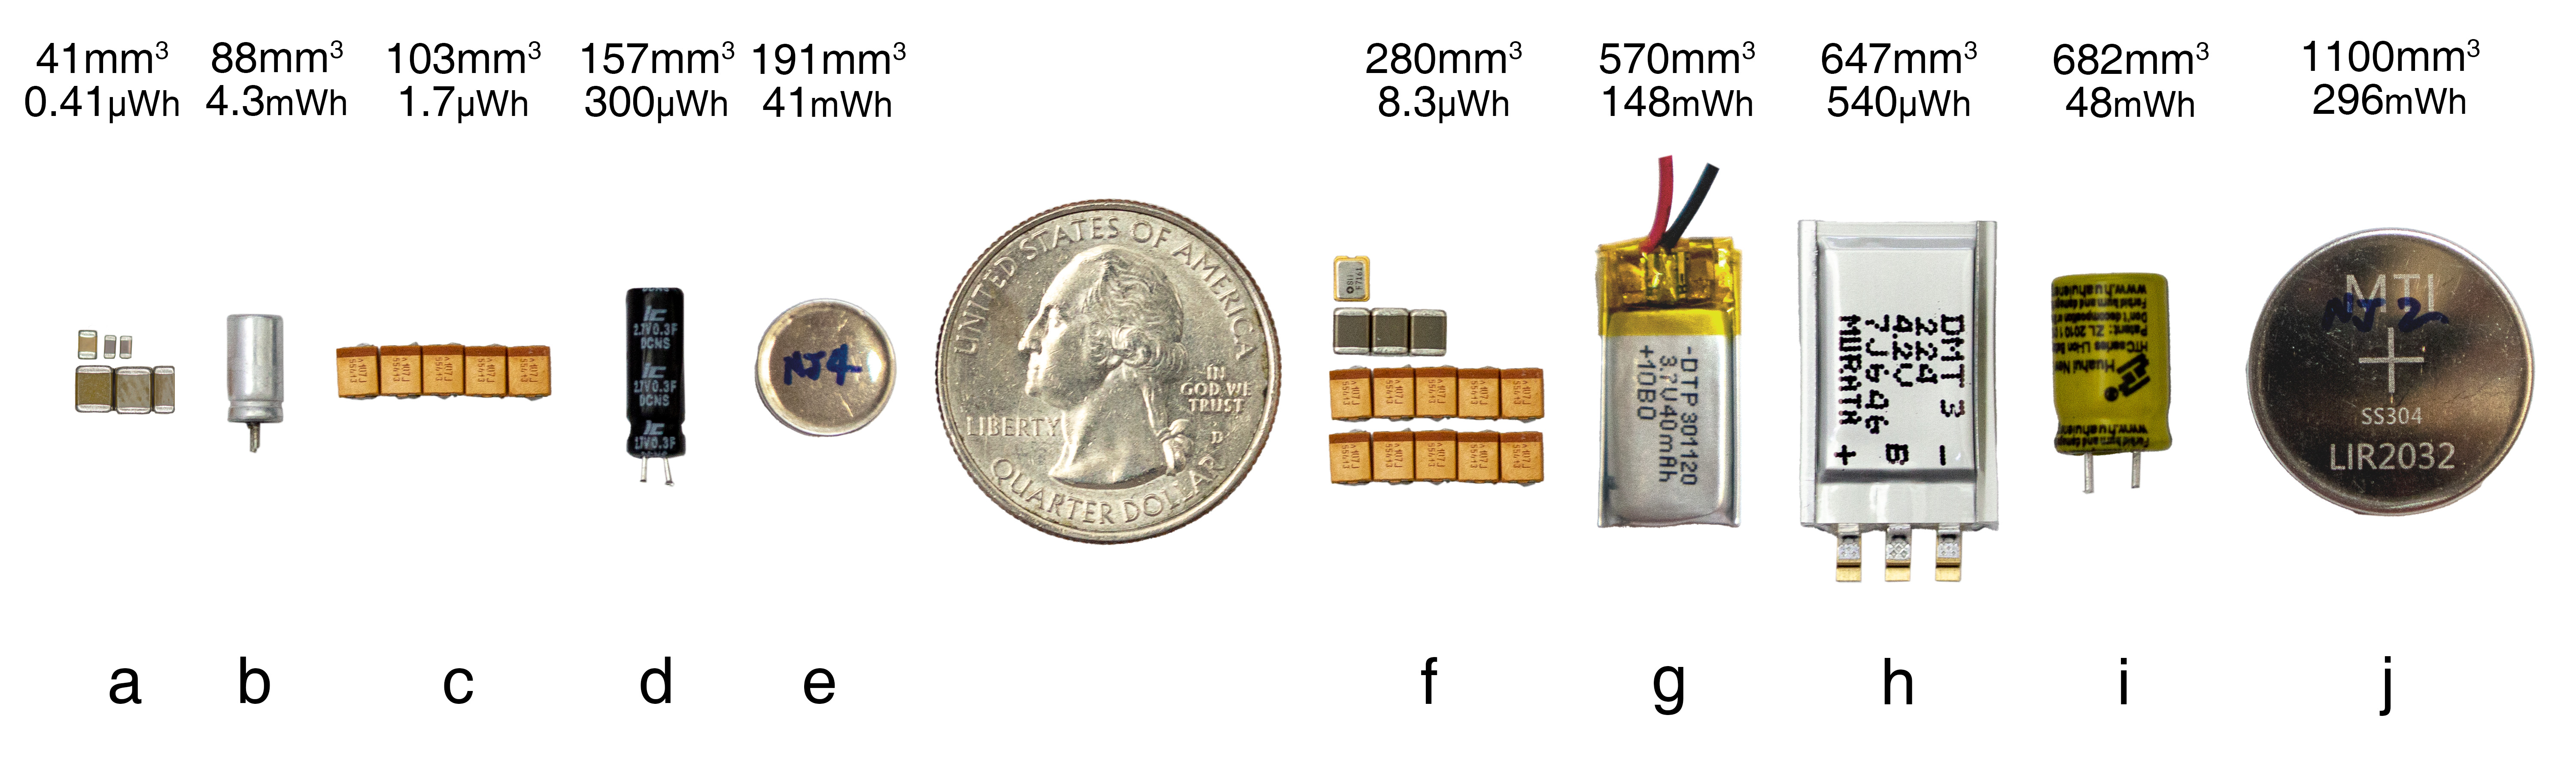
\includegraphics[width=\columnwidth]{figs/batteries/cap_lto_size_compare}
  \caption{
    A size comparison of energy storage methods including capacitors, supercapacitors, and batteries.
    \normalfont
    They are ordered left to right, by their
    (total) volume. Total volumes and energy storage are listed above the respective device.
    Configuration
    \textbf{(a)}, \textbf{(c)} and \textbf{(f)} represent the energy storage configurations used
    in the Flicker platfrom with BLE and several sensors~\cite{hesterFlicker17}, the Solar Monjolo~\cite{campbellEnergy14} and the Capybara temperature
    monitor and alarm~\cite{colinReconfigurable18}, which have total
    capacitances and energy capacities of 119\si{\micro\farad} (0.41\si{\micro\Wh} at 5~V), 500\si{\micro\farad} (1.7\si{\micro\Wh} at 5~V)
    and 8.8\si{\milli\farad} (8.3\si{\micro\Wh} at 2.6~V), respectively. Capacitors
    \textbf{(d)}~\cite{illinoisCap} and \textbf{(h)}~\cite{murataCap} are large
    supercapacitors available on the Capybara platform and have the
    capacitances and energy capacities of 300\si{\milli\farad} (300\si{\micro\Wh} at 2.7\si{\volt}) and 220\si{\milli\farad}
    (540\si{\micro\Wh} at 4.2\si{\volt}) respectively.  Devices \textbf{(b)} and \textbf{(i)} are 
    small LTO battery cells with 1.8\si{\milli\Ah} (4.3\si{\milli\Wh} at 2.4~V) and 20\si{\milli\Ah} (48\si{\milli\Wh}
    at 2.4\si{\volt}) capacity respectively~\cite{LTODatasheet2}. Devices \textbf{(e)} and \textbf{(j)} are small prototype Li-ion coin cells with 11\si{\milli\Ah} (41\si{\milli\Wh} at 3.7~V) and 80\si{\milli\Ah} (296\si{\milli\Wh} at 3.7~V) respectively~\cite{millibatNimbus}. Device \textbf{g} is a traditional Lithium Polymer pouch cell with 40\si{\milli\Ah} (148\si{\milli\Wh} at 3.7~V)~\cite{sparkfunPouch}.
    The LTO battery \textbf{(b)} and the Li-ion coin cell \textbf{(e)} are among the smallest of all configurations of energy storage
    presented here and also provide one to two orders of magnitude more energy capacity
    compared to \textbf{(f)}, the largest supercapacitor presented.
  }
\end{definefigure}

\begin{definefigure}{fig:battery:ragone}
\centering
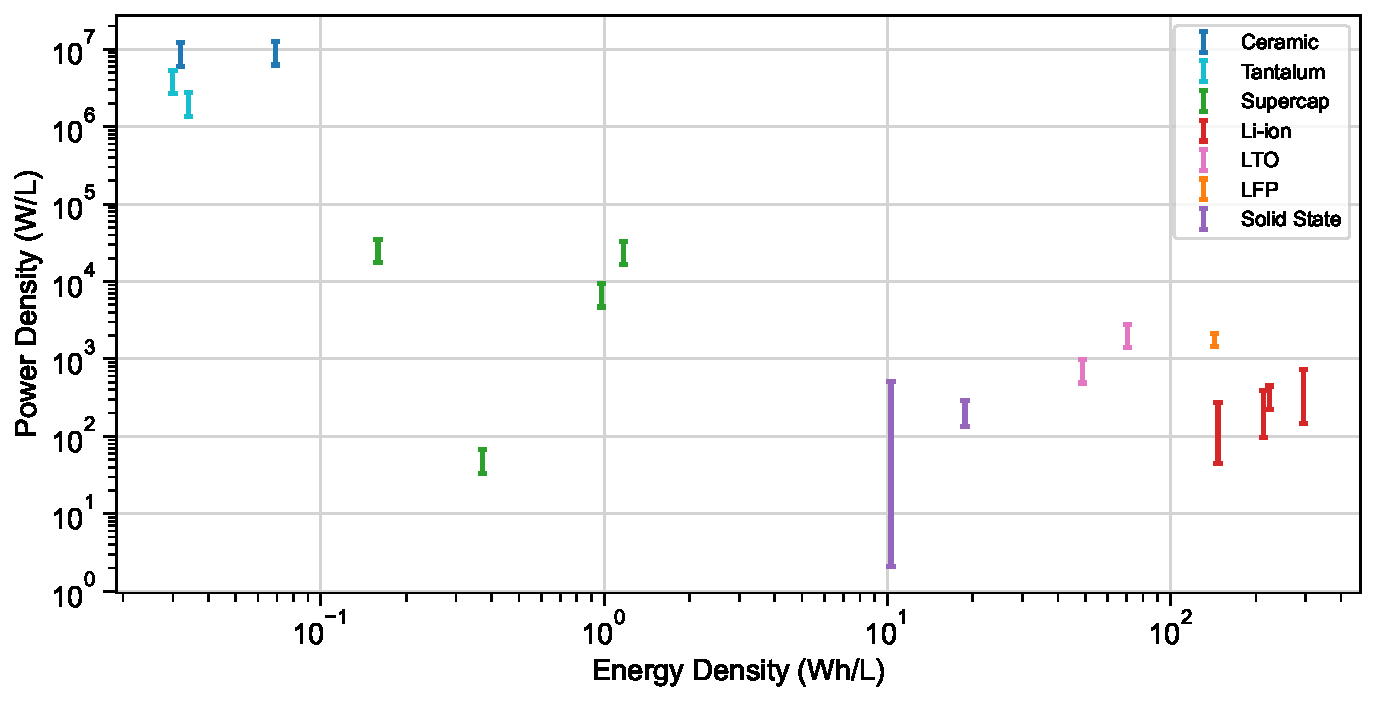
\includegraphics[width=\columnwidth]{figs/ragone}
\caption{Ragone plot for components listed in \cref{tab:battery:cost}, in log-log scale. A ragone plot directly compares power and energy density for different devices. Ceramic and tantalum capacitors are very power dense, but provide abysmal energy density. Batteries provide superior energy density, are less power dense. Supercapacitors exist between these two extremes. Even though batteries do not provide comparable power density to either capacitors or supercapacitors, they can still provide sufficient power for common wireless sensor workloads, like operating a short or long range radio.}
\end{definefigure}

\begin{definefigure}{fig:battery:eperd}
\centering
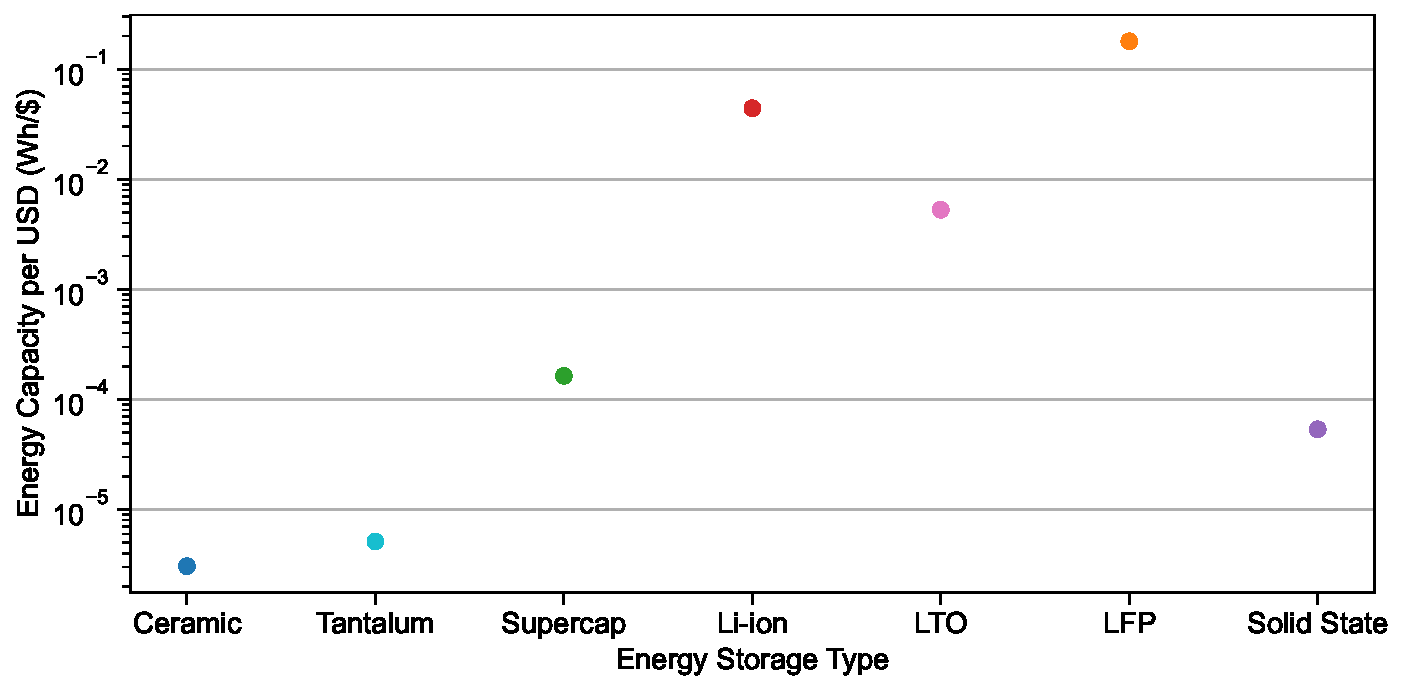
\includegraphics[width=\columnwidth]{figs/energy_per_cost.pdf}
\caption{
    Average energy capacity for various technologies selected in \cref{tab:battery:cost}, normalized by price in USD. Wherever possible, component costs were determined by their price in the United States. In regards to energy capacity, batteries offer 3-5 orders of magnitude more energy capacity per dollar than ceramic and tantalum capacitors. Batteries also offer 2-3 orders of magnitude more capacity than supercapacitors.
}
\end{definefigure}

\chapter{Utilizing Capacity for Untethered Image Sensing}
\label{cha:permacam}

\section{Evaluating an Existing System through Simulation}

\section{Capacity-focused Redesign of an Existing System}


\section{Summary}
\chapter{Utilizing Capacity for Capable Computation and Inference}
\label{cha:capability}

\section{Compute and Communication Energy Tradeoff}

\section{Increasing Compute Capability with an Accelerator}

\section{Summary}

\chapter{Conclusion}
\label{chap:conc}

\section{The Local Compute versus Transmit Trade-Off}

For Camaroptera, the decision to include local inference to filter out non-interesting images was worth it due to cost of transmitting images. This is not necessarily the case with Permacam, where the costs of doing the inference and transmitting images is about equal.
Embedded computing is improving in power efficiency at higher rate than active radios.


\subsection{Power Trends}

Figure: Energy per bit vs \ssi[per-mode=symbol]{\micro\ampere\per\mega\hertz} for radio/processor over time.

\subsection{Computing Trends}
Introduction and improvement of low power embedded accelerators for DSP and neural net inference. What are the trends? How to compare with conventional Cortex M cores and each other?

\subsection{The Constant Need for More Energy}
As computing efficiency increases, sensor data processing complexity will continue to increase, resulting in sensors that do more for the same amount of power. These sensors will require all the energy they can get. 

\section{What Primitives will Future Energy Harvesting Sensors Need?}

A wish list for future sensor design primitives.

\begin{enumerate}
    \item Coulomb counting for energy income and used energy
    \item Separate power domains for state preservation and active operation
    \item More memory and memory protection (virtual memory?) for more sophisticated programs and usability
    \item Parallel interfaces on low power SoCs
\end{enumerate}

\section{Conclusion}


% \appendix
% \chapter{More Monticello Candidates}

\printbibliography
\end{document}
